% vim:spelllang=en_us:spell
% Author: Marek Filip 2022

\chapter{Introduction}

When we look at cryptocurrencies, there is a very lucrative market. That is why people have always found new ways to make money from trading cryptocurrencies. There are many trading strategies for cryptocurrencies available, but no such strategy survives both rising (bull) and falling (bear) market. That is why there is a need for adaptive strategies that can prosper through both of them.

I will explore the idea of the adaptive trading strategies for cryptocurrencies in this thesis. Firstly we need to find a way how to predict if the market will go up or down. Then we need to apply sufficient trading strategies regarding the percentage probability of market going up or down. That is the basic idea.

To get to this point I will explore the current trading strategies that are used for trading cryptocurrencies. Analyze current simulation tools available today and analyze the historic trading data to find some patterns. Looking at current state of adaptive strategies for cryptocurrencies is also necessary.

\subsection*{Organization}

The rest of this work is divided into several chapters.

Firstly, there is the chapter \ref{chapter-background}, which gives the reader a sufficient theoretical background that is required to understand the later chapters of the thesis. In the chapter \ref{chapter-trading-stategies} I look at the existing trading strategies and analyze their effectiveness. In the chapter \ref{chapter-simulation-tools} several existing simulation tools are explored and compared. During chapter \ref{chapter-data-analysis} the backlog of cryptocurrency trading data provided by the supervisor is analyzed and the important events summarized.

After these chapters the thesis becomes more oriented towards the project goal of the backtester itself. In chapter \ref{chapter-strategy-proposals}, several adaptive strategies are proposed. In chapter \ref{chapter-implementation} the design, development and implementation of the backtester itself is detailed. After that, in chapter \ref{chapter-experiments} the proposed adaptive trading strategies are tested out using the developed backtester and results are evaluated. Finally, limitations and further improvements of practical deployment are discussed in chapter \ref{chapter-limitations-and-improvements}


\chapter{Background}
\label{chapter-background}

There are some prerequisites that the reader must be familiarized with in order to understand the thesis. The basic knowledge of what a cryptocurrency is must be explained. As well as clear understanding of some terms that are regularly used in the thesis.

\subsection*{List of Terms Generally Used in the Thesis and Among Crypto Investors}
\begin{itemize}
    \item Best strategy = A strategy that yields the most money -- has the best profit.
    \item Bear market = A market in which prices are falling, encouraging selling.
    \item Bull market = A market in which prices are rising, encouraging buying.
    \item Fiat currency = Government-issued money.
    \item spread = Difference between buy and sell value of an asset.
    \item OHLCV = open, high, low, close, value -- type of candlestick data
    \item MA = moving average, usually refers to smooth moving average.
    \item SMA = smooth moving average.
    \item ROI = Return of investment.
    \item FOMO = Fear of missing out.
    \item FUD = Fear, uncertainty, doubt.
    \item API = Application programming interface.
\end{itemize}

\section{What is a Cryptocurrency?}
\emph{Cryptocurrency} is a digital currency that is secured by cryptography~\cite{investopedia-cryptocurrency}. There are algorithms in place that make it nearly impossible to counterfeit or double-spend the currency. Cryptocurrencies are based on a decentralized networks based on the blockchain (see \ref{blockchain}) technology. Because of this the cryptocurrencies are not issued by any central authority (unlike conventional currency). This makes them theoretically immune to government interference or manipulation.

\subsection*{Types of Cryptocurrency}
\emph{Bitcoin} is the original and to this day the most popular and valuable cryptocurrency. It was invented by an anonymous person called \emph{Satoshi Nakamoto} in 2008 via a white paper~\cite{satoshi}. As of 12th January 2022, there are over 18.9 million bitcoins in circulation with a total market capitalization of around \$810 million~\cite{coinmarketcap}, making it roughly 40\% of the total cryptocurrency market.

Each new cryptocurrency claims to have different function and specification. New cryptocurrencies are created daily. Most are not lucrative to investors at all while others surprise the market with their new innovations. For example, Ethereum's \emph{ether} markets itself as a gas for their underlying smart contract\footnote{\url{https://www.investopedia.com/terms/s/smart-contracts.asp}} platform. Another example is Ripple's \emph{XRP} which aims to facilitate international bank transfers. New cryptocurrencies started to rise due to bitcoin's many unsuitable aspects.

\label{stablecoins-ref}
A \emph{stablecoin} is another important type of cryptocurrency. It aims to offer price stability and is backed by a reverse asset\footnote{\url{https://www.investopedia.com/terms/r/reserve-assets.asp}} like the US dollar. They attempt to offer the best of both worlds---the instant processing and security of privacy payments of cryptocurrencies, and the non-volatile character of fiat currencies~\cite{investopedia-stablecoin}.

\subsection*{What Is FIAT money?}
Fiat money or currency is money that is issued by the government and is not backed by any gold or other physical commodity. Its value is derived between the relationship of supply and demand and the stability of the government that issued it~\cite{investopedia-fiat}. It represents today's currencies of the world. Many crypto enthusiasts believe that cryptocurrencies will replace fiat currencies in the future.

\subsection*{Blockchain}
\label{blockchain}
Blockchain or a distributed ledger\footnote{\url{https://www.investopedia.com/terms/d/distributed-ledger-technology-dlt.asp}} is a digital database that is shared and synchronized across a distributed network consisting of very large number of computers~\cite{investopedia-blockchain}. Distributed networks eliminate the need for central authority to keep a check against manipulation. You can see the blockchain's basic structure in Figure \ref{blockchain-figure}.

\begin{figure}[!hbt]
    \centering
    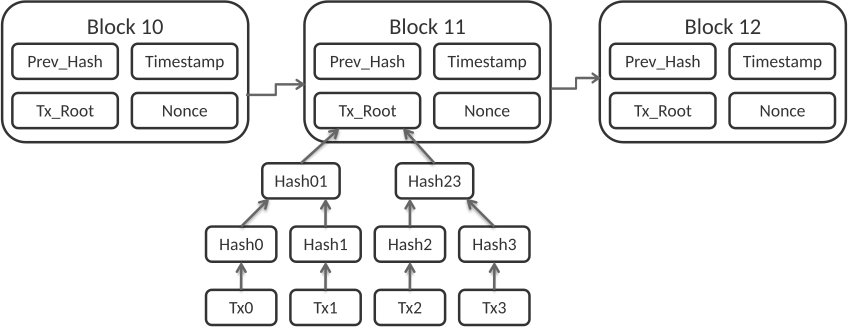
\includegraphics[width=\columnwidth]{figures/Bitcoin_Block_Data.png}
    \caption{Blockchain structure, attribution: Wikimedia TODO: citace}
    \label{blockchain-figure}
\end{figure}

\section{What Are Bear and Bull Markets?}
While you may know that the bear and bull markets stand for falling and rising markets, there is more to these terms that must be explained. The origin of the terms themselves is believed to be tied to the way the two animals attack their opponents. A bull thrusts its horns up, while a bear swipes its pawns downwards~\cite{investopedia-bull-market}.
Herd behavior is important to consider when talking about the terms.

\subsection*{Bear Market}
As growth prospects wane and expectations are unmet, prices decline~\cite{investopedia-bear-market}. Bear markets are viewed as pessimistic with investors scared to open new positions. But to talk about bear or bull market we usually ascribe longer time periods than the usual and always present volatility of the crypto market. For example when China declared all of the cryptocurrency transactions illegal~\cite{china-ban}, a fall of crypto markets quickly ensued.

A bearish investor or bear is then a type of investor that believes that a specific coin is likely to decline in the future~\cite{investopedia-bull}.

\subsection*{Bull Market}
Bull markets are characterized by optimism, investor confidence and expectations in strong results that will continue for a long period of time~\cite{investopedia-bull-market}. FOMO\footnote{Fear of missing out.} is present among investors. Both bull and bear markets are hard to define, bull market is usually specified to occur when prices rise by $20\%$ after a previous $20\%$ drop and before another $20\%$ drop---these values are defined for stock markets only, so the margins should be higher for the volatile cryptocurrency market.

A bullish investor or bull is a type of investor that believes that a specific coin is likely to rise~\cite{investopedia-bull}.

\section{What Is a Trading Strategy?}
Trading strategy is traditionally defined as a systematic methodology that is used for buying and selling the selected assets in a market. It is based on predefined rules and criteria that are used to execute a trading decision~\cite{investopedia:trading-strategy}.

In this thesis, a trading strategy is considered a method which tells us whether to buy or sell on given day based on indicators, such as the current cryptocurrency price, or total market capitalization.

\chapter{Trading Strategies for Cryptocurrencies}
\label{chapter-trading-stategies}

There are various trading strategies available regarding cryptocurrencies.
In this chapter we will go through those that are considered the most well-known and consider
their ups and downs.

\section{HODL}

This is the strategy that is one of the most prominent in the cryptocurrency market, especially by beginners to trading.
It is jokingly derived from misspelling of the word "hold". The original post by the user GameKyuubi~\cite{hodl-post} containing the misspelling was originally posted on 18th December 2013, from which it quickly spread on.

HODL or "hodl on for dear life" has become a slogan among crypto enthusiasts, representing long-term approach to cryptocurrency trading. It implies that the novice traders are not successful in timing the market so they should simply hold the coin until the prices significantly rises.

Cryptocurrency maximalists keep HODLing, because they believe that cryprocurrencies will eventually replace the government-issued fiat currencies as the basis of all economic structures~\cite{investopedia-hodl}.

\section{Rebalance}
Rebalancing is the process of realigning the weightings of portfolio of assets---in our case cryptocurrencies. It involves periodically buying or selling the assets in portfolio so that the original level of asset allocation is maintaine~\cite{investopedia-rebalancing}.

For example if we set portfolio allocation 50/50 to BTC and ETH coins. And the BTC coin rised by 20 \% so that the new ratio would be 70/30, we would sell the 20 \% of the BTC and for the value we got we would buy additional ETH coins, so that the ratio is again 50/50.

Rebalancing gives investors the opportunity to sell high and buy low. It takes gains from high-performing investments and reinvests them in areas that have not yet grown that much.

One study~\cite{portfolio-rebalancing}, conducted by the Shrimpy Team, has found that rebalancing beats hodl by a median of $64\%$. The analysis was performed with 1-year period real trading data.

There many types of rebalancing strategies. We will look at some of them now.

\subsection*{Periodic Rebalancing}
This is the simplest rebalancing to use. The rebalance happens after a fixed amount of time. For cryptocurrencies it makes sense to set shorter time due to rapid price fluctuations, something like 1 day. An example of periodic rebalancing can be seen in Figure \ref{periodic-rebalance-figure}.

\begin{figure}[!hbt]
    \centering
    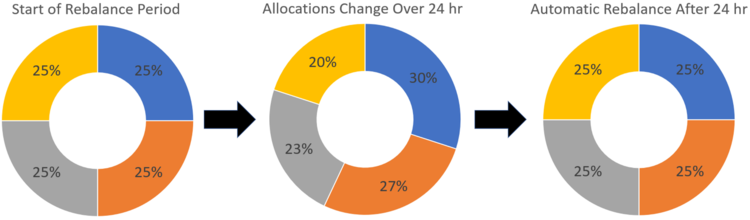
\includegraphics[width=\columnwidth]{figures/periodic-rebalance.png}
    \caption{Periodic rebalance visualization, attribution: Shrimpy~\cite{portfolio-rebalancing}.}
    \label{periodic-rebalance-figure}
\end{figure}

\subsection*{Threshold Rebalancing}
A more interesting approach is threshold rebalancing where we set some threshold deviation. When an allocation deviates by that set threshold from the original allocation, a rebalance happens, setting all the allocations to their original values~\cite{portfolio-rebalancing}.

Let's say we once again have 50/50 BTC/ETH allocations. Let's set the threshold deviation to $20\%$. If the price of BTC or ETH reaches over 60\% or under 40\%, a rebalance takes place. 20\% out of 50\% is 10\%, that is why the rebalance happens at those points. When both coins grow or decline in the same rate, no rebalance happens.

An example of threshold rebalancing can be seen in Figure \ref{threshold-rebalance-figure}.

\begin{figure}[!hbt]
    \centering
    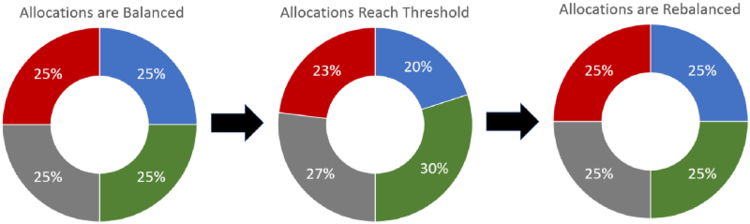
\includegraphics[width=\columnwidth]{figures/threshold-rebalance.png}
    \caption{Threshold rebalance visualization, attribution: Shrimpy~\cite{portfolio-rebalancing}.}
    \label{threshold-rebalance-figure}
\end{figure}

\subsection*{Assumptions}
\label{rebalance-assumptions}
One study around rebalancing has been already mentioned, let's look into some of them in more detail now. The studies~\cite{portfolio-diversity} and~\cite{diversify-perform-better} conducted by the Shrimpy organization have found some interesting results. Both of the studies took into account only periodic rebalancing. They have found that the shorter the time period for rebalance, the better the results, maximizing them at 1 hour period. The other interesting discovery was that if the portfolio had more assets in it---was more diversified---the better were the results. The diversification really took advantage of the sell high buy low formula.

Another study~\cite{rebalancing-strategy} confirmed that a portfolio with a larger number of assets performs better. Some other interesting facts have been observed during the simulations that improve the performance of the portfolio:
\begin{itemize}
    \item Equal weightings of the allocated assets.
    \item Assets that are uncorrelated or negatively correlated with each other. That means if one rises, the other should go down.
    \item Assets that have similar rates of return, though volatility also improves the performance.
\end{itemize}

\section{Dollar Cost Averaging}
Dollar Cost Averaging (DCA) is a strategy often recommended to the beginner investors. The investor makes periodic purchases of the asset in an effort to reduce the volatility of the market. This removes much of the detailed work needed to time the market in order to make purchases at the best price.

Through studies~\cite{DCA-study} it seems that the advantage of DCA lies more in the reduced psychological effort in order to time the market than in the actual results. Single buy-and-hold strategy seems to outperform DCA in more cases.

Sometimes DCA is used as a mean to invest into trusted assets on weekly/monthly basis---when employees get money. It is also used in some employment plans\footnote{For example the American 401(k) plan} across the world.

\section{Day Trading}
Day trading are the investors that buy and sell the same asset over the span of one day. They might even buy and sell the assets multiple times. They mostly use technical analysis of the market to achieve this goal. It is not recommended for beginner investors to choose this type of trading as it is much more risky than strategies described before.

\section{Range Trading}
\label{section-range-trading}
Asset move in certain ranges, as you can see in Figure \ref{trading-range-figure}. Range trading assumes that and tries to take guesses where are the limits using candlestick charts and support and resistance levels. Investors want to buy when prices reach the support level and sell when they reach the resistance level~\cite{5types-of-daytrading}. The support and resistance levels can be seen in Figure~\ref{sup-and-res-levels}.

\begin{figure}[!hbt]
    \centering
    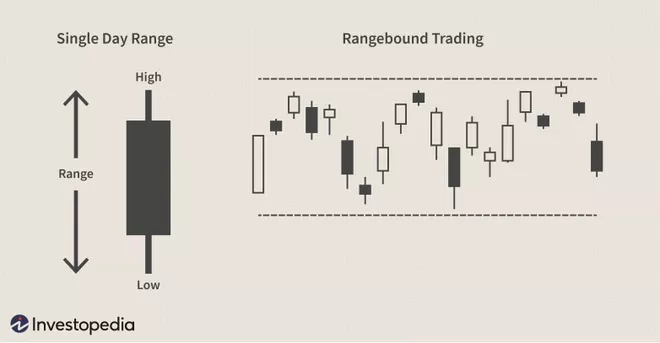
\includegraphics[width=\columnwidth]{figures/trading-range.png}
    \caption{Trading range visualization, attribution: Investopedia~\cite{investopedia:trading-range}}
    \label{trading-range-figure}
\end{figure}

\begin{figure}[!hbt]
    \centering
    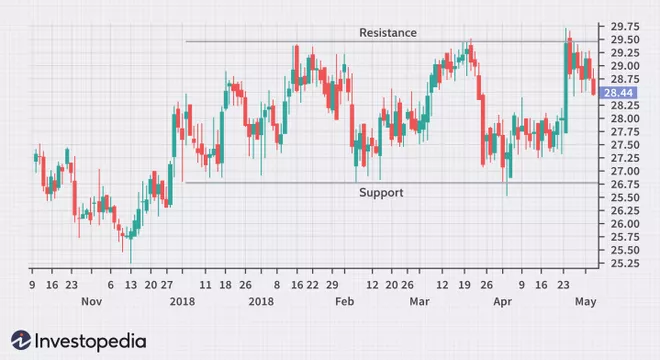
\includegraphics[width=\columnwidth]{figures/dotdash-final-trading-range.png}
    \caption{Support and resistance levels, attribution: Investopedia~\cite{investopedia:trading-range}}
    \label{sup-and-res-levels}
\end{figure}

\section{Scalping}
\label{section-scalping}
In scalping you try to profit from very small price movements over short periods, you might exit a trade seconds after entering it. It is best to use automated bots to increase the buying frequency. Scalpers take advantage of increased trading volume to profit. They want to exit before any news or short-term fluctuation changes the market's view of the coin~\cite{best-crypto-daytrading}.

It is needed to have a large bankroll to use this strategy effectively. Since the return of investment is really low, the amount gain must be significant enough. It also needs to cover trading fees.

In Figure \ref{scalping-figure} it can be seen how scalping can take quick and short advantages of the market.

\begin{figure}[!hbt]
    \centering
    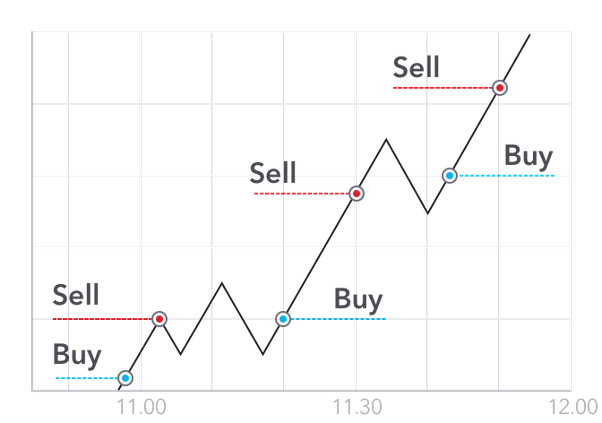
\includegraphics[width=\columnwidth]{figures/scalping.png}
    \caption{Scalping visualization, attribution: Quora~\cite{best-crypto-daytrading}}
    \label{scalping-figure}
\end{figure}

\section{Automated Trading Systems or Bots}
\label{bots}
Automated trading systems---also referred as algorithmic trading---allow investors to set specific rules for enter and exit of a trade that can be automatically executed via computer program. Some platforms claim that 70\% to 80\% of trading done comes from the automated systems~\cite{investopedia-bot-trading}.

One of the advantages is that the automated trading systems take emotions out of the trading---they only work on a specific criteria. The automated trading systems need to use software or APIs available from the broker. The outcome made in this thesis is expected to be used by some automated trading system.

Automated trading systems are one of the only options to use when considering strategies like scalping due to the ease of getting in and out of a trade in seconds without room for failure. The software also allows backtesting the chosen strategy on historical data from which it can be seen how well it does perform.

\section{Arbitrage}
Arbitrage involves buying cryptocurrency in one market and selling it for higher price in another one. Since the cryptocurrency market is usually unregulated, anyone can make an exchange. This can lead to major differences in the spread of the asset.

There are two types of arbitrage when it comes to cryptocurrencies. The first one focuses on finding prices mismatches across different trading pairs on a single exchange. The other is the one that was already described---locating significant price differences on multiple exchanges. Both types take advantage of an automated trading system that monitors the exchanges and looks for price differences. In Figure \ref{arbitrage-figure} you can see how the first type can be profitable.

Regarding the second type of exchange. In January a legendary \emph{kimchi premium}\footnote{\url{https://www.investopedia.com/terms/k/kimchi-premium.asp}} happened. Bitcoin traded almost 40\% higher on the Korean exchanges that the US exchanges. This lead to arbitrage investors taking advantage of this fact, buying bitcoin on US exchanges and selling it on the Korean ones for profit~\cite{hodlbot:day-trading-cryptocurrency}.

\begin{figure}[!hbt]
    \centering
    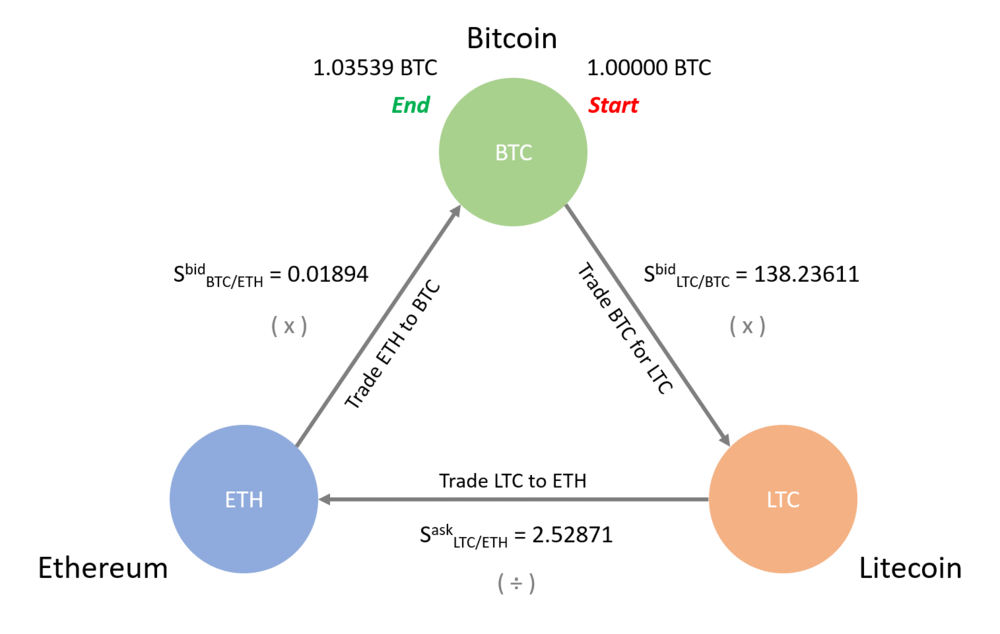
\includegraphics[width=\columnwidth]{figures/arbitrage.png}
    \caption{Arbitrage execution via multiple trading pairs, attribution: HodlBot~\cite{hodlbot:day-trading-cryptocurrency}}
    \label{arbitrage-figure}
\end{figure}

\section{Stablecoin Trading}

When talking about different trading strategies, the focus is usual on the method of the trategy, not the asset themselves. But when it comes to specific thing like stable coints, there is an opportunity to handle them in such a way to generate profits for us.
The term stablecoin has already been explained in \ref{stablecoins-ref}. It is a coin which has its value pegged to some external reference.

For example it was found in~\cite{make-money-stablecoins} that a de-pegging of stablecoins happens periodically often as a result of temporary shock to the crypto system. During those events profit can be made when trading pegged and de-pegged stablecoins between each other. The author chose DAI and USDC pair for their experiments. It was shown that between August 2019 and March 2020 the spread between DAI and USDC has been fluctuating between 2 to 3\%. Advantage could be taken of this fact---selling DAI for USDC when the price is high and buy it back for USDC when the price returns to the peg.

One thing to remember is to only trade when the spread is sufficient so that the trading fees won't make the profit diminish.

\chapter{Existing Simulation Tools for Testing Trading Strategies}
\label{chapter-simulation-tools}

In this chapter different simulation tools, their application, usefulness and differences, are discussed. We must distinguish few types of simulation tools when talking about them. When a novice investors first sets foot in the cryptocurrency market, they might be startled by the complexity of the market. They want to learn, but maybe they do not want to lose all their money in the process. That is the perfect opportunity for a manual simulated tool. Investors can invest fake virtual money while all of the market's trading data is accurate and up to date.

\section*{Types of cryptocurrency simulators}

\begin{enumerate}
    \item Cryptocurrency market games
    \item Virtual trading simulators
    \item Backtesting simulation tools
\end{enumerate}

\emph{Cryptocurrency market games} are games that have less emphasis on the trading skills and more on the entertainment of trading. They are mostly fun way to compete with your friends or strangers. The player that creates the strongest portfolio is considered the best. The winner is then the player with the best investments at the end of the specific game.~\cite{top-stocks-crypto-trading-simulators}.

\emph{Virtual trading simulators} are simulators where users can closely track the real market and actively trade cryptocurrencies for virtual profit~\cite{top-stocks-crypto-trading-simulators}. The main goal is to use the simulated experience for building and improving the real life trading skills of the user. You can test-drive and backtest your strategy here.

\emph{Backtesting simulation tools} are similar to the virtual trading simulators in a way, that it aims to make its users better at trading. While the conventional trading simulators only work in real time, there are simulation tools where its users can input chosen strategy and see it run across multiple years of historical data and see how it performed in seconds. This is the type of simulation tools that will be used in this thesis. It basically uses backtesting for the cryptocurrency strategy's validation.

\section{What is Backtesting?}
The section was inspired by this source~\cite{backtesting-crypto-trading-strategies}.

Backtesting means applying a trading strategy or some analytical method on a historical data and analyzing the performance of the current strategy or method. If the strategy shows promise, the trader may use it in a live environment on an exchange. Backtesting does not guarantee future results, but can be a good indicator and filter the effective strategies from the ineffective ones. Backtesting can also detect recurring patterns and exploit those patterns for profits.

\subsection*{Discretionary Backtesting}
Discretionary backtesting is a manual form of backtesting. The trader manually places buy and sell order with each signal they receive. They trader may decide to conduct the testing using software such as TradingView\footnote{\url{https://www.tradingview.com/}}.

The trader will set a strategy in place, then he will press the replay button (shown in Figure \ref{tradingview-figure}) and select period of history to test on. The trader will then make discretionary decisions to buy or sell based on the signals.

Manual testing is a great way to control trader's emotions since they may feel the same emotions as in live environment. The disadvantage is that it is quite time-consuming. Trader may run a test for hours only to find out it was not a good strategy (though this result is also valuable). Secondly the amount of data the trader can test the strategy on is limited.

\begin{figure}[!hbt]
    \centering
    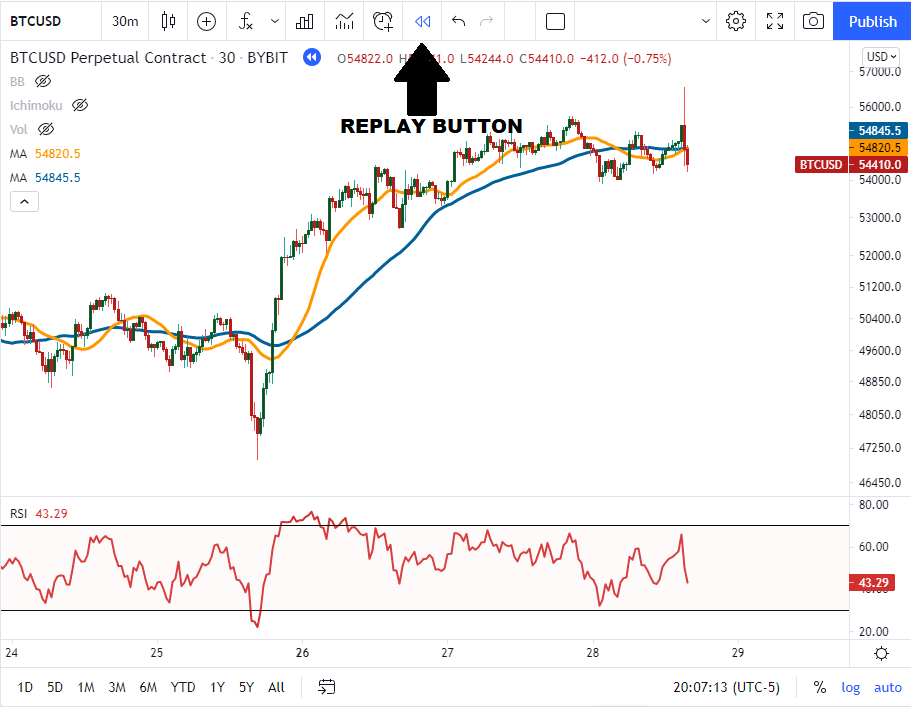
\includegraphics[width=\columnwidth]{figures/tradingview-replay.png}
    \caption{TradingView replay functionality, attribution: TradingView~\cite{backtesting-crypto-trading-strategies}}
    \label{tradingview-figure}
\end{figure}

\subsection*{Systems Backtesting}
Systems backtesting offers the trader the true power of technology. Systems traders will have a strategy coded and the program will test the strategy against the historical data while generated statistics of the achieved results in manner of seconds. This will show the trader useful statistics about the strategy and help him decide if it is robust and well-performing enough to use in a live environment.

The challenge of systems backtesting is to have sufficient technical knowledge on how to create such algorithmic strategies. And also the analytical knowledge to determine if the strategy performed well or not.

\subsection*{Automated Backtesting}
Automated or \emph{algorithmic} trading refers to traders who use a computer program to execute a trade, as explained in \ref{bots}. Backtesting of strategies can also be automated this way and is usually just another name for systems backtesting. We automate the results to arrive at helpful statistic to help us determine effective strategies. It is conducted using a programming language.

\subsection*{Simulated Backtesting}
Simulated backtesting simply means running a test over a historical data that simulates the real market environment. In this example the system is market environment and the model is the simulated environment.


\section{Data Requirements for Backtesting}
Systems traders will want to simulate the real-world data as closely as possible. Trading costs such as commissions, exchange spreads and slippages can chew away the expected returns. This costs can throw off the backtest results if ignored.

Both \emph{candlestick} and \emph{order book data} are used in backtests, though order book data is usually more reliable.

\subsection*{OHLCV Candlestick Data}
\label{ohlcv-candlestick-data}
OHLCV stands for Open-High-Low-Close-Volume, you can see how they can be represented in Figure \ref{OHLCV-figure}. The candlestick data itself is visualized in Figure \ref{candlestick-figure}. It is essentially a spreadsheet of price data of the chart time frame. If you pull the candlestick data for the daily chart of Bitcoin, you will receive each day's open, high, low and close price data. If you request 1-minute data, the spreadsheet will include each minute's open, high, low and close price for Bitcoin on that particular day.

OHLCV abbreviations explained~\cite{kaiko-ohlcv}:
\begin{itemize}
    \item Open: Price at which the asset started at the time interval.
    \item High: Highest price reached during the time interval.
    \item Low: Lowest price reached during the time interval.
    \item Close: Price at which the asset ended after the time interval.
    \item Volume: Quantity of asset bought or sold, displayed in base currency.
\end{itemize}

\begin{figure}
    \centering
    \begin{subfigure}[t]{0.45\textwidth}
        \centering
        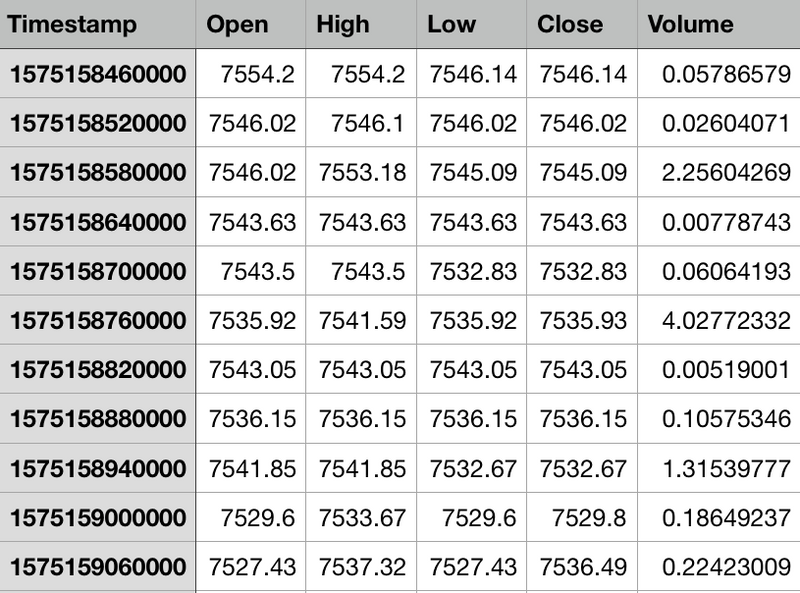
\includegraphics[width=\textwidth]{figures/OHLCV-data.png}
        \caption{How can OHLCV data look like, attribution: Kaiko~\cite{kaiko-ohlcv}}
        \label{OHLCV-figure}
    \end{subfigure}
    \hfill
    \begin{subfigure}[t]{0.45\textwidth}
        \centering
        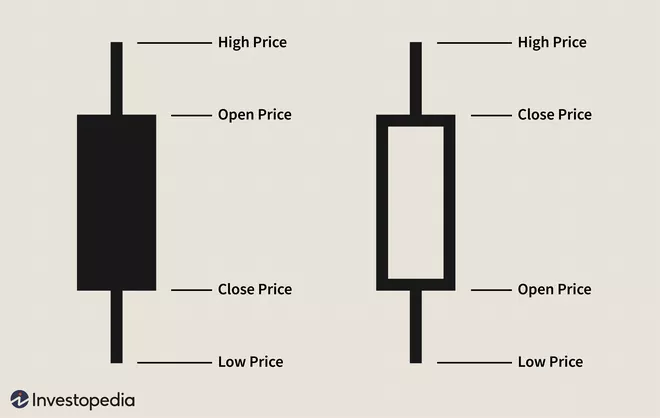
\includegraphics[width=\textwidth]{figures/candlestick-data.png}
        \caption{Candlestick explained, attribution: Investopedia~\cite{investopedia:candlestick-charts}}
        \label{candlestick-figure}
    \end{subfigure}
    \caption{OHLCV Candlestick Data}
\end{figure}

There are several imperfection to the OHLCV candlestick data. Firstly, there is no information which prices have been traded for which volume. Additionally, if a trader has a large account, there might not be enough cryptocurrency available to trade without moving the market price---negatively impacting the backtest results. Traders typically use candlestick data because it is easiest to acquire.

\subsection*{Order Book Data}
An order book is one of the best data sources and resolves some challenges of the candlestick data. It includes snapshots of the market, including the market's price, volume and depth. With this type of data traders have a better representation of what orders are available at any given time.

It allows testers to simulate bid-ask spread, slippage and liquidity when testing a particular strategy. All of these unavailable to testers using candlestick data. The challenge with order book data is that it is hard to come by. There is tremendous amount of data with order book snapshots so the exchanges choose not to hold the data, as it would be too expensive to store. Therefore usually the developers needs to collect and store the data from the exchange themselves or access the snapshots through a third-party service.

\section{Performance Analysis}
\label{performance-analysis}
This section was again inspired by the~\cite{backtesting-crypto-trading-strategies} source.

Performance of the given trading system or strategy is commonly gauged against parameters such as profit and loss (P\&L), success ratio, and Sharpe ratio.

\subsection*{Profit and Loss -- P\&L}
Once the desired strategy has been created and backtest executed, the big number traders will be interested in is the profit. The backtest should spit out P\&L analysis by trade and day. That way an equity curve can be created, showing what the balance would have been if it were traded live. Equity curve is just a time series chart showing what the value of the account would have been after each passed day.

P\&L analysis also generates the size of the average winning and the size of the average losing trade. Taking the ratio of those two averages you get a useful average risk-to-reward ratio. For example if the average winning trade is \$100 and the average losing trade is \$50 you get a $1:2$ risk-to-reward ratio.

\subsection*{Success Ratio}
The success ratio is the win ratio of the strategy. Let's say a strategy makes 100 trades. If 72 of those trades are profitable, it has 72\% success (or win) ratio. By itself the ratio does not tell much and might be misleading. It is best coupled with the average winner and the average losing trade ratios mentioned in P\&L.

For example, a success ratio of 58\% and 1:2 risk-to-reward ratio indicates a very good strategy.

\subsection*{Sharpe Ratio}
This subsection was sourced from~\cite{investopedia:sharpe-ratio}

The Sharpe ratio, developed by \emph{William F. Sharpe}, is used to understand the return of an investment (ROI) compared to its risk. The ratio is the average return earned in excess of the risk-free rate per unit of volatility or total risk.

$$Sharpe\ ratio = \frac{R_p - R_f}{\sigma _p}$$
where:
\begin{itemize}
    \item $R_p$ = return of portfolio
    \item $R_p$ = risk-free rate
    \item $R_p$ = standard deviation of the portfolio's excess return
\end{itemize}

Generally, the greater the value of the Sharpe ratio, the more attractive the risk-adjusted return. The yield for the US Treasury bound is often used as the risk-free ratio. One of the limitation of the Sharpe ratio is that it assumes that the returns are normally distributed, which is simply not true.

\section{Popular Simulation Tools}
Some popular and easily available simulation tools are Holderlab\footnote{\url{https://holderlab.io/}}, Zenbot\footnote{\url{https://github.com/DeviaVir/zenbot}}, Gekko\footnote{\url{https://gekko.wizb.it/}}, Altrady\footnote{\url{https://www.altrady.com/}}, and Binance's Python backtesting\footnote{\url{https://www.binance.com/}}.

\section{What type of cryptocurrency simulation tool should we use?}
When looking at the explored simulation tools it is clear that an automated backtesting program will be used to test the proposed adaptive trading strategy. I will use the OHLCV candlestick data provided by the supervisor and look for order book data if needed. When evaluating the strategy I will not only look at P\&L ratio, but also the average winner and losing trades, risk-to-reward ratio and more complex tools like Sharpe ratio.

\subsection*{Programming Language}
When looking at possible languages to use I consider available libraries and frameworks. I decided to use Python for its many available trading and backtesting frameworks and because of my personal experience with it for data collection.

\subsection*{Backtesting Frameworks}
Let's look at the available backtesting frameworks for Python. Using frameworks might make things easier for us. Between the candidates for backtesting frameworks I put PyAlgoTrade, bt, backtrader, zipline and Blueshift. Apart from that \emph{numpy}\footnote{\url{https://numpy.org/}}, \emph{pandas}\footnote{\url{https://pandas.pydata.org/}} and \emph{matplotlib}\footnote{\url{https://matplotlib.org/}} libraries will be probably of great use for general data transformation and visualization. Following section's lines have been inspired by~\cite{python-backtesting-frameworks} source.

When reviewing backtesting frameworks it's always good to ask what asset classes you are trading, what data frequency and detail is required and what order type should be supported by the chosen framework. Some frameworks go beyond backtesting and include live trading capabilities that make it easier for potential deployment.

The framework should have a way to consume trading data in a convenient way. It should calculate a broad range of risk and performance metrics as explained in \ref{performance-analysis}, including the max drawdown and Sharpe and Sortino ratios.

Computer resources may be a problem sometimes. Traders can opt for frameworks with distributed or parallel processing in those scenarios. When it comes to strategy optimization, program may attempt to find the optimal parameters for each technical indicator, testing various combinations. In portfolio context, the program may try to find the best weighting of every asset in the portfolio for the ideal rebalance.

We will now look at a few backtesting frameworks for Python and lightly compare them. The common capabilities of the frameworks is that they are event driven, with flexible licenses, having decent number of pre-defined technical indicators and standard performance metric calculation, visualization and reporting capabilities.

\emph{PyAlgoTrade}\footnote{\url{https://github.com/gbeced/pyalgotrade}} is a fully documented framework with paper and live trading capabilities. Its data support includes Yahoo! Finance, Google Finance, NinjaTrader and any type of CSV-based time series.

\emph{bt}\footnote{\url{https://pmorissette.github.io/bt/}} is used to test quantitative trading strategies. It allows traders to easily create strategies that mix and match different algorithms. It aims to save developers time re-inventing the wheel and instead focus on the strategy development.

\emph{backtrader}\footnote{\url{https://www.backtrader.com/}} is a feature-rich backtesting framework. It allows you to focus on writing reusable trading strategies, indicators and analyzers rather than on building the infrastructure itself.

\emph{Blueshift}\footnote{\url{https://blueshift.quantinsti.com/docs/}} is a platform to research and test systematic investment stategies. It is asset-class and instruments agnostics. It is not meant for HFT---high frequency trading.

\emph{Zipline}\footnote{\url{https://github.com/quantopian/zipline}} is a event-driven system for backtesting. It is accessible through the browser-based IPython Notebook interface, which makes it available to developers who do not prefer the command line.


\chapter{Trading Data Analysis}
\label{chapter-data-analysis}

In this chapter the history data of cryptocurrency market is analyzed. We try to find trends and patterns that we can then use to our advantage when coming up with an adaptive trading strategy.

\section{Types of Analysis}
This section was inspired by the~\cite{binance:bitcoin-price-history} source.

Before we analyze the cryptocurrencies themselves, let's take a look at ways how to analyze them. There are generally three possible methods: technical, fundamental and sentiment analysis. Each type has its strength and weaknesses. Combining them together creates a clearer picture.

\subsection*{Technical Analysis -- TA}
The main focus here is on the historical price and volume data. We can create 50-day moving average (SMA) by taking the last 50 days' prices and averaging them. If a cryptocurrency has been trading under its 50-day SMA for a few weeks and suddenly breaks through, it may be seen as a sign of possible recovery.

\subsection*{Fundamental Analysis -- FA}
Fundamental analysis takes its merits from the fundamental, intrinsic value of a project or cryptocurrency. It concentrates on internal and external factors to try to establish the asset's actual value. For example, you could take a look at daily cryptocurrency's transaction to measure the network's popularity. If the number of transactions rises over time, it may suggest the value of the project and that its price may rice.

\subsection*{Sentiment Analysis -- SA}
Sentiment analysis is the use of market sentiment to predict the price movements. Market sentiment represents the feelings and mood of investors towards an asset. These are typically categorized into bullish and bearish sentiments. A significant increase in google searches about purchasing some cryptocurrency may suggest a market sentiment.

\section{Bitcoin Price Analysis}
This section was inspired by the~\cite{binance:bitcoin-price-history} source.

First thing to analyze is Bitcoin in particular. No other cryptocurrency has such an impact on the cryptocurrency market and still remains to have impact to this day. Bitcoin has started it all, so it is only appropriate to analyze it completely. We can see the linear and logarithmic graphs in Figures \ref{btc-linear-figure} and \ref{btc-log-figure} respectively.

While the linear graph shows us the actual price changes, the logarithmic graph is also useful to us. It shows us relative price increases of the Bitcoin. It represents a percentage increase in price, change from \$10 to \$20 is the same as \$1000 to \$2000 since the investor will in both cases gain a profit of 100\%. Because of this, logarithmic scale is usually often for technical analysis.

\begin{figure}[!hbt]
    \centering
    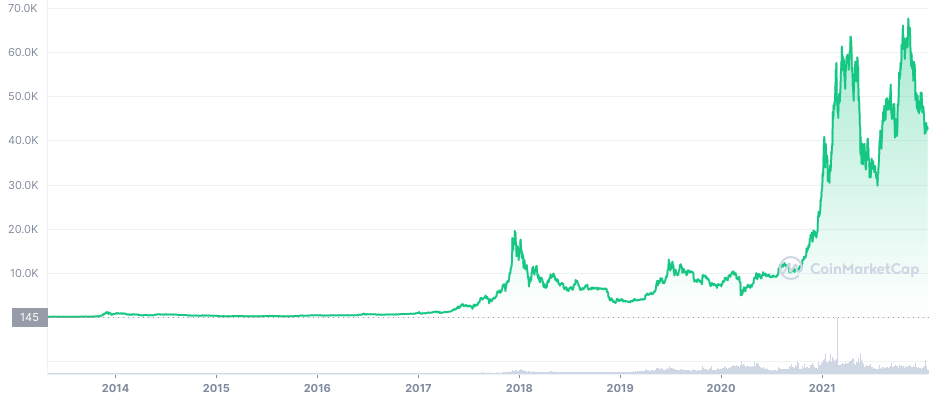
\includegraphics[width=\columnwidth]{figures/BTC_ALL_linear.png}
    \caption{Bitcoin linear price graph, attribution: CoinMarketCap~\cite{coinmarketcap}}
    \label{btc-linear-figure}
\end{figure}

\begin{figure}[!hbt]
    \centering
    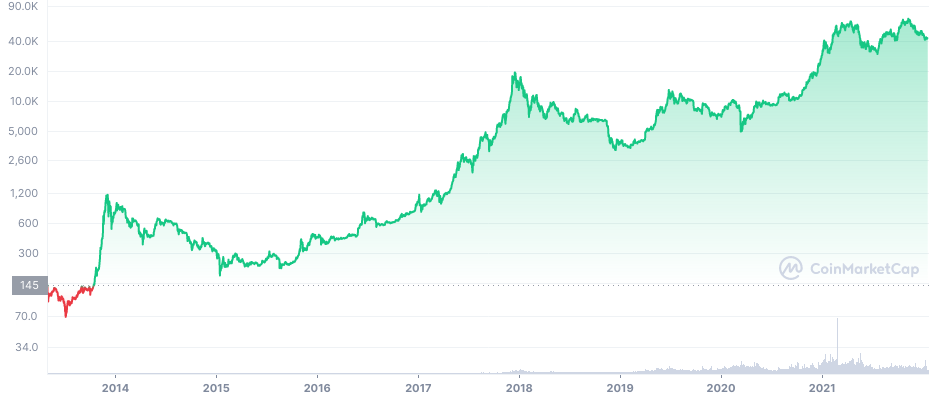
\includegraphics[width=\columnwidth]{figures/BTC_ALL_log.png}
    \caption{Bitcoin logarithmic price graph, attribution: CoinMarketCap~\cite{coinmarketcap}}
    \label{btc-log-figure}
\end{figure}

\section{Data Analysis Provided by Supervisor}

TODO:

\begin{itemize}
    \item Bitcoin's difficulty has been increased + Elon Musk tweet -> correlation
    \item China banned cryptocurrencies
    \begin{itemize}
        \item how long did the recession last and how it developed
    \end{itemize}
    \item why we do not see small recession as bear market
    \item most cryptocurrencies are driven by bitcoin change, that means they are driven by world events.
\end{itemize}

\chapter{Adaptive Trading Strategy Proposals}
FIXME: Most of the proposals are also mentioned in the chapter Experiments, should I still include it? Maybe I could write the theory here and leave the experiments only for implementation and results. Some not implemented strategies could also be put here.

\label{chapter-strategy-proposals}

\section{Proposals}

\subsection*{Bull Market Behavior}
During the possible Bull Market we hold coins, rebalance and buy more of them.

\subsection*{Bear Market Behavior}
During Bear Market we transfer our holding to stablecoins (in certain percentage) so that the market fall does not impede us.

\section{Bitcoin Risk Metric}
This term was most probably coined and invented by Benjamin Cowen on his youtube channel \footnote{\url{https://www.youtube.com/channel/UCRvqjQPSeaWn-uEx-w0XOIg}}, or at least it is mostly associated with his figure. It is an alogirthm that prescribes a certain risk value, between 0 and 1, to each day of bitcoin price. It takes into account the maximum value that has already occured so far in the history. This strategy is often favourable by DCA. Depending on the risk scale, you either invest more if the risk is lower and invest less (or not at all) if the risk is high.

The metric oscillates between highs and lows. There have been 5 high points of the metric since the year 2015.

\subsection*{DCA}
\label{DCA}

\section{Adjusted Risk Metric}

\section{Other Optimizations}

\subsection*{24H Volume---Correlation}

\subsection*{Number of Larger Drops in Market}

\subsection*{Machine Learning Time Series Optimizations}

\section{Short-term Trading}
When focusing on short-term trading, range trading and scalping discussed in Sections \ref{section-range-trading} and \ref{section-scalping} respectively. We try to guess the support and resistance levels.

When talking about technical analysis, we need to make support and resistance levels into an account. They can be predicted in several ways. Round numbers are taken into account, like \$50 and \$100, since investors usually put stop orders at such whole number points. These points then serve as resistance levels since it takes very large number of purchases to absorb the sales. Moving average can be used to estimate the levels, too, as you can see in the Figure \ref{ma-support-resistance}. Other indicators include the golden ratio, number of touches and others. This paragraph has been inspired by the \cite{investopedia:support-and-resistance} source, where more detailed information can be found.

In the thesis, moving averages are used to estimate the support and resistance levels and make according trades.

\begin{figure}[!hbt]
    \centering
    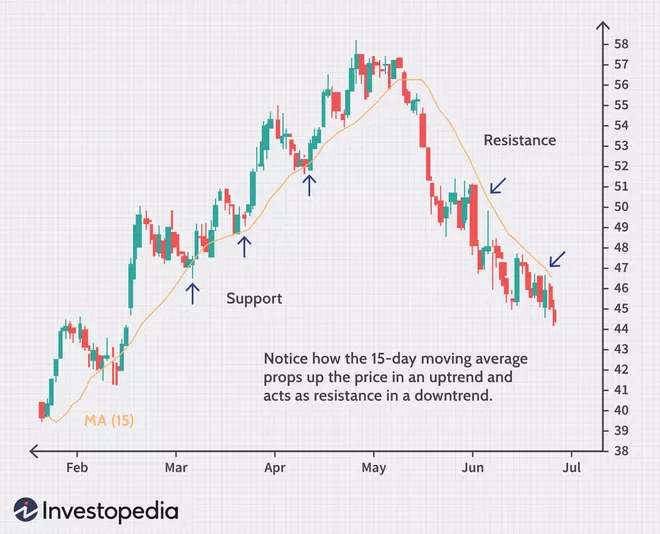
\includegraphics[width=\columnwidth]{figures/ma-support-resistance.png}
    \caption{Expected support and resisted levels computed by a moving average. Attribution: Investopedia \cite{investopedia:support-and-resistance}}
    \label{ma-support-resistance}
\end{figure}



\chapter{Adaptive Strategy Design and Implementation}
\label{chapter-implementation}

\section{Design}
During my search, I initially tinkered with several frameworks to test out their capabilities. The basic idea was that if a framework would prove satisfactory I would use it and tweak it to my needs so I do not reinvent the wheel again.

Alas, during my tinker with Python frameworks as \emph{PyAlgoTrade}, \emph{backtrader} or \emph{zipline}, the frameworks were either outdated or they did not meet my needs of adaptive strategies.

\subsection*{vectorbt}
One of the more promising frameworks was the \emph{vectorbt} library. I did a few basic graphs and strategies with it like HODL and MA (moving average) crossover, the examples can be seen in the code. Unfortunately, the library also proved to be insufficient, or more well put, overly complicated, when it came to my needs. Rather than spending days trying to understand a few functions from the library I decided it would be faster to create my own backtesting framework that would serve the strategies perfectly while still understanding the inner working of the framework completely. This point was also supported by the thesis supervisor and discussions I found on the internet \cite{reddit:custom-backtester}.

\subsection*{General Design}
The general idea is to build a backtesting command line interface (CLI) application. It takes input arguments from the CLI or a configuration file and passes it to the argument parser. The parser parses the arguments, it then gets all the requested data either via API calls, or if the data already exists, fetch them from the local filesystem. All of the arguments, data range and data itself is then converted to a trading data data structure and passed to the simulator. The simulator calls several strategies and aggregates the results into a strategy result data structure. That is then passed to the Plotter class. Plotter plots the results and optionally prints out the strategies stats. The visualization can be seen in Figure \ref{structure-diagram}.

\begin{figure}[!hbt]
    \centering
    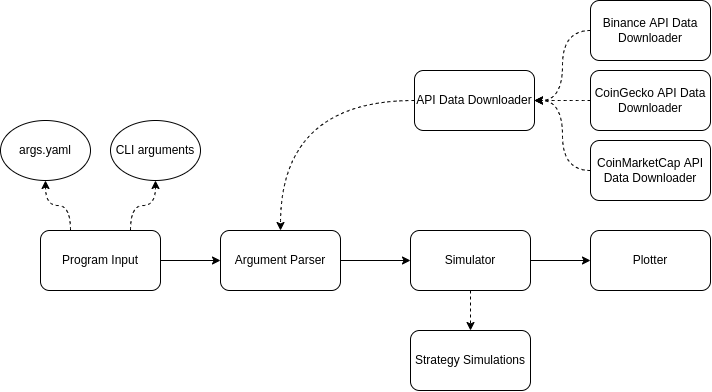
\includegraphics[width=\columnwidth]{figures/structure-diagram.png}
    \caption{General design structure of the backtester}
    \label{structure-diagram}
\end{figure}

\subsection*{Strategy Class}
All strategies are derived from the base strategy abstract class. The class provides the common functions, constants and data initialization. The inherited classes usually overwrite the \texttt{execute\_step} method which does a singular step of the strategy (1 day if the data is days apart).

One interesting strategy in particular is the StrategyMerger class that allows merging the behavior of several strategies. It basically combines the \texttt{execute\_step} of the strategies in the order they are defined.

Strategy classes with their most important attributes are shown in Figure \ref{figure-strategy-class-diagram}

\begin{figure}[!hbt]
    \centering
    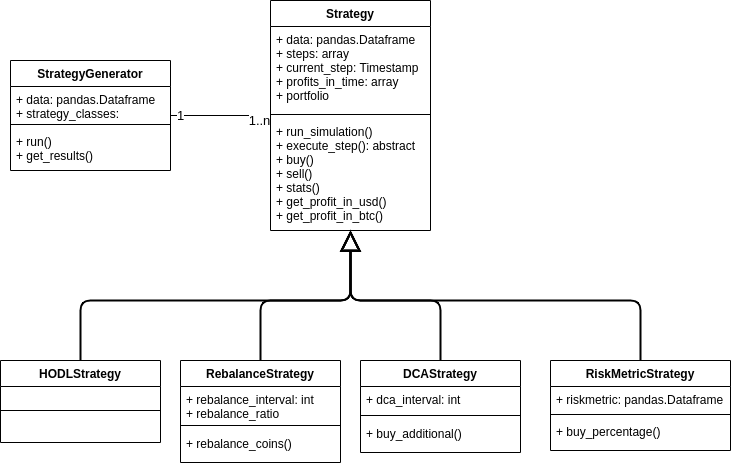
\includegraphics[width=\columnwidth]{figures/strategy-class-diagram.png}
    \caption{Class diagram of strategies of the backtester}
    \label{figure-strategy-class-diagram}
\end{figure}


\section{Fetch of Trading Data}
Initial trading data that was used for the experiments were initially provided by the supervisor. Due to their incompletness and due to them being out-of-date, a need for more complete data was created.

I designed the data fetch into a few categories. I then researched each category and chose the best suited API provider for the thesis.

\subsection*{OHLCV data}
I needed OHLCV 5 minute and 1 hour data to test various strategies this way. After going through some recommendations I settled with Binance API\footnote{\url{https://www.binance.com/en/support/faq/c-6}} for OHLCV data since I already had an account with them. All that is needed are public and secret API keys to make the requests.

\subsection*{Historical BTC}
One of the disadvantages of Binance API is that it only goes as far back as it started. That is to the July 2018. When calculating things like bitcoin risk metric it is advantegous to have earlier data available. To this end I used the free and public CoinGecko API\footnote{\url{https://www.coingecko.com/en/api/documentation}}. The \texttt{coins/market\_chart} endpoint was ideal for this use case.

Historical data have daily interval and include only the price and volume of each day, so it is not the standard OHLCV data. The data dates to the year 2013.

\subsection*{Global Metrics}
Another need due to the alternative risk metric was created for the total crypto market capitalization. This data is not present in Binance nor CoinGekco API. The perfect information was found at CoinMarketCap website\footnote{\url{https://coinmarketcap.com/charts/}}. After a bit of web scraping I got to the original API call\footnote{\url{https://api.coinmarketcap.com/data-api/v3/global-metrics/quotes/historical?interval=1d}}.

The data includes several useful metrics. The most important one is the total market capitalization of each day dating to year 2013. Other useful ones are 24 hour volume and bth/eth dominance for each day.

\subsection*{Implementing the Fetch}
Ideally, we would get all of our data from single API provider. Unfortunately, I have found no single provider that provides the needed data in the requested format.

\texttt{python-binance}\footnote{\url{https://pypi.org/project/python-binance/}} 3rd party module is used to ease the getting the data from Binance API. \texttt{pycoingecko}\footnote{\url{https://pypi.org/project/pycoingecko/}} does the same thing for the CoinGecko API. Data got from CoinMarketCap are fetched via the interface of the 3rd party module \texttt{requests}\footnote{\url{https://pypi.org/project/requests/}}

The only API that needs public and private keys is the Binance API. The keys are hidden in the \texttt{.env} file and got from the configuration library called \texttt{python-decouple}\footnote{\url{https://pypi.org/project/python-decouple/}}

\section{Usage}
FIXME: Move this section to appendices---manual

Usage is defined in the standard environment of bash command line interface. All needed commands are provided by the Makefile and can be listed by running \texttt{make}.

Install dependencies:
\begin{minted}{bash}
make installdeps
\end{minted}

Run the project:
\begin{minted}{bash}
# using Makefile
make run

# using the module itself + argument file
python -m backtester -f args.yaml

# using the module itself + CLI arguments
python -m backtester -s 2020-01-01 -e 2022-01-01 -i 1d -p BTCUSDT ETHUSDT
\end{minted}

\section{Data Input}
There are a few different program arguments that are needed to be specified.

Pairs are used to select the cryptocurrency pairs we want to trade. Since Binance requires both of the assets to be cryptocurrencies we cannot select \$USD. Closest asset to it is the token that is pegged against \$USD, USDT. So if you want to choose trading pair where the price of bitcoin and \$USD is compared, choose BTCUSDT.

Starting and ending date do exactly as the name suggests, they define the data range in which the data is fetched. The interval argument defines the OHLCV interval between each data, it uses Binance abbreviations and there are several possible values. The values I mostly used were 5m and 1h interval, that means that the OHLCV data fetched will be either 5 minute or 1 hour apart.

Due to a possbile long list of argument values, the arguments can be saved into a file in the YAML\footnote{\url{https://yaml.org/}} format. Its schema is then validated and arguments dictionary got via the \texttt{schema}\footnote{\url{https://pypi.org/project/schema/}} and \texttt{PyYAML}\footnote{\url{https://pypi.org/project/PyYAML/}} Python libraries respectively.

Among optional arguments belongs the logging level. It defines the logging level used for logging that informs the users of filesystem manipulations, simulation progress and results, or errors and debug information. Defaultly it is set to level INFO.

\section{Other Helpful Structures}

\subsection*{Plotter}
\texttt{plotly}\footnote{\url{https://pypi.org/project/plotly/}} is used for plotting the final graphs. It works natively with the dataframe data used in \texttt{pandas}.

\section{Deployment and Development}
During the development of the project, code standards were enforced via various programming tools, such as linters, formatters, pre-commit and CI checks. All the selected technologies can be viewed in the repository of the project.

\subsection*{Containerization--Docker}
For ease of development and deployment, the project has been packaged into a container that can be run via the docker command. This way anyone can easily try out the program or develop it having only the required docker command installed.

Other containerization benefits include:
\begin{itemize}
    \item Runtime Environment Agnosticism
    \item Isolation from other processes
    \item Portability
    \item Ease of delivery
    \item Scalability
\end{itemize}

\subsection*{Virtual Environment}
Other option on how to develop the project is to use the Python virtual environment. \texttt{virtulenv}\footnote{\url{https://pypi.org/project/virtualenv/}} is used in the project, but other tools like \texttt{venv}\footnote{\url{https://docs.python.org/3/library/venv.html}} and \texttt{conda}\footnote{\url{https://docs.conda.io/en/latest/}} could be used.

After activating the environment and installing the required packages via \texttt{pip}. The project is ready to be run and developed. Of course the project can be developed without ever activating the virtual environment. Conflicting Python packages and versions may cause a dependency problem though. This way the whole project is seperated from the local installation of the opearting system.

\subsection*{Makefile}
Makefile is used to put a common interface for all the other commands and tools. It is recommended to use the targets from Makefile for running and developing the project. All lint, format, containerization, testing, latex translation targets are located there.

\subsection*{Testing}
Simple testing was set up using the pytest framework\footnote{\url{https://docs.pytest.org/}}. The test files can be found in the \texttt{tests} folder. The tests serve to verify the basic functionality of the implemented trading strategies.

\chapter{Adaptive Strategy Experiments}
\label{chapter-experiments}

Before we can dive into the individual adaptive strategy experiments we need some traditional strategies that we can compare the adaptive results against. HODL and Rebalance will serve as such strategies. Both are very simple to implement and highly used. That makes them the perfect candidate for this purpose.

All of the graphs decpited in the section have been produced by the implemented backtester program, proving its usefulness.

\section{Evaluation Strategy}
Before we get to the individual experiments, the main process for evaluating the experiments must be described. There are 2 caveats to this process. Firstly we need to define the strategy that tells the probability of market going up or down, let us call it the risk metric. And secondly we need to find the optimal strategy that works with this metric---that means an algorithm that decides what to do when the metric is at such level and what to do if it is in a different level---finite state machine.

Basically, the thesis can be split into a function and a finite state machine. The function's inputs is the today date and some kind of other data used for calculating the metric (e.g. historical price of Bitcoin). Function then calculates the risk (limited between <0,1>) for the current day and passes the value to the finite state machine. The automata then decides on what to do, taking its previous steps into the account.

\subsection*{Finite State Machine behavior}
The most basic idea is to transfer the coins to stablecoins when the risk is near the high boundary and transfer back to coins when it is again nearing the lower boundary. Alternatively, when using the DCA strategy \ref{DCA}, we do not invest when the risk is high and invest more money the lower the risk is.

\subsection*{Evaluation variables}
When looking at the evaluation, we need to keep in mind the variables that can influence the results greatly. Firstly the chosen cryptocurrencies may differ quite a lot, and choosing different quantity of them. The other obvious variable is date range. When evaluating we will also try to look at the ranges that experienced only bull or bear market, not just the long data ranges. Finally the data interval---as in 5m or 1d---may influence the data.

Some DCA portfolio can look like this:
\begin{itemize}
    \item $Risk \ge  0.7$: Do not invest.
    \item $0.6 \le Risk < 0.7$: Invest sum x1.
    \item $0.5 \le Risk < 0.6$: Invest sum x2.
    \item $0.4 \le Risk < 0.5$: Invest sum x3.
    \item $0.3 \le Risk < 0.4$: Invest sum x4.
    \item $0.2 \le Risk < 0.3$: Invest sum x5.
    \item $0.1 \le Risk < 0.2$: Invest sum x6.
    \item $Risk < 0.1$: Invest sum x7.
\end{itemize}

For the evaluation, a coin to stablecoin transfer has been chosen for the profit evaluation. In the following chapters the metric calculation is discussed. The profit evaluation is detailed when needed.

Coin to stablecoin ratios can look like this:
\begin{itemize}
    \item $Risk \ge  0.7$: All capital is converted to stablecoins.
    \item $0.6 \le Risk < 0.7$: 60\% converted.
    \item $0.5 \le Risk < 0.6$: 40\% converted.
    \item $0.4 \le Risk < 0.5$: 20\% converted.
    \item $0.3 \le Risk < 0.4$: Capital is in coins only.
    \item $0.2 \le Risk < 0.3$: Capital is in coins only.
    \item $0.1 \le Risk < 0.2$: Capital is in coins only.
    \item $Risk < 0.1$: Capital is in coins only.
\end{itemize}


\subsection*{Used Datasets}
We will be testing with a few portfolios. Every portfolio will start with base 1000\$ USD budget. Portfolio A is using only the bitcoin and ethereum, these two assets show promising and stable growth and have been the 2 biggest contributors to total market capitalization. As of May 1st 2022, the two cryptocurrencies contribute to almost 62\% of total market capitalization~\cite{coinmarketcap:globalmetrics}. Both cryptocurrencies of the portfolio date back to the earliest Binance data point.

For portfolio B, the top 20 coins (not tokens) listed on the CoinMarketcap~\cite{coinmarketcap} (as of 1st May 2022), based on market capitalization and disregarding stablecoins, have been chosen. The total age of the portfolio is much younger, dating back to 2020. The difference between the portfolios should show how the strategies change depending on the portfolio size and disparity.

Portfolio A is used to find tweaks in the strategies. Portfolio B is used to find out how the strategy results changes from portfolio B.

Assets (tickers) of the portfolio A:
\begin{itemize}
    \item Bitcoin (BTC)
    \item Ethereum (ETH)
\end{itemize}
Longest possible date range of portfolio A: 17th July 2017--today

Assets (tickers) of the portfolio B:
\begin{itemize}
    \item Bitcoin (BTC)
    \item Ethereum (ETH)
    \item BNB
    \item XRP
    \item Solana (SOL)
    \item Terra (LUNA)
    \item Cardano (ADA)
    \item Dogecoin (DOGE)
    \item Avalanche (AVAX)
    \item Polkadot (DOT)
    \item Polygon (MATIC)
    \item NEAR Protocol (NEAR)
    \item Tron (TRX)
    \item Litecoin (LTC)
    \item Bitcoin Cash (BCH)
    \item Cosmos (ATOM)
    \item Algorand (ALGO)
    \item Stellar (XLM)
    \item Monero (XMR)
    \item Ethereum Classic (ETC)
\end{itemize}
Longest possible date range of portfolio B: 14th October 2020--today (limited by the NEAR Protocol)

Intervals of 1 day will be used for long-range backtesting and 5 minute for backtesting in range of several days.

Assets (tickers) of the portfolio C:
\begin{itemize}
    \item Bitcoin (BTC)
\end{itemize}

Portfolio C serves to backtest the bitocoin risk metric against its main driver.


\subsection*{Benchmark Strategies}
Our benchmark strategies are going to be HODL and periodic Rebalance. Periodic rebalance is going to be set to 1 day or 5 minute interval, depending on the data interval. If the adaptive strategy outperforms the mentioned strategies, it has a good potential to be a good strategy. HODL and rebalance is often used by starting investors, so this outperforming these is a step in a good direction.

We will invest 1000\$ every time to make strategies comparable. Performance of the strategies in various settings can be seen in Figures \ref{figure-benchmark-1} and \ref{figure-benchmark-2}, in linear and logarithmic scale. We can see that the periodic rebalance interval matter. We will use the shortest interval as suggested by the assumptions in Section \ref{rebalance-assumptions}. One interesting find is that the rebalance strategy actually performs worse than HODL when used with the portfolio B.

\begin{figure}[!hbt]
    \centering
    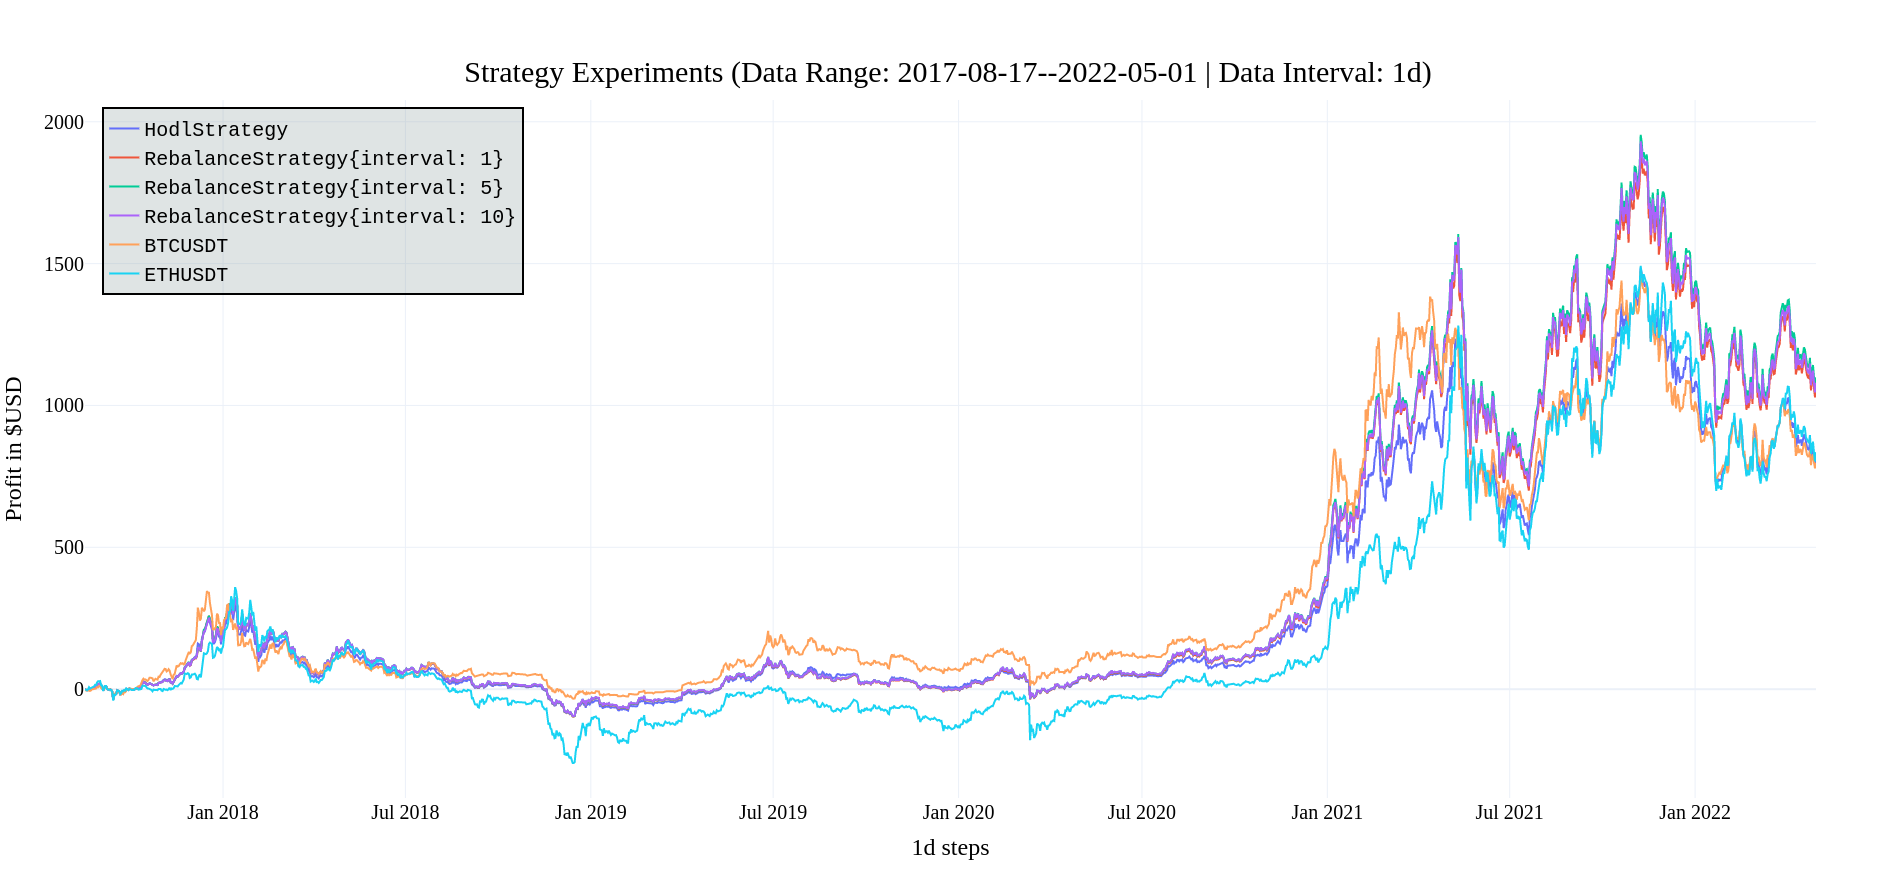
\includegraphics[width=\columnwidth]{figures/benchmark-A.png}
    \caption{Portfolio A: HODL and Rebalance performance}
    \label{figure-benchmark-1}
\end{figure}

\begin{figure}[!hbt]
    \centering
    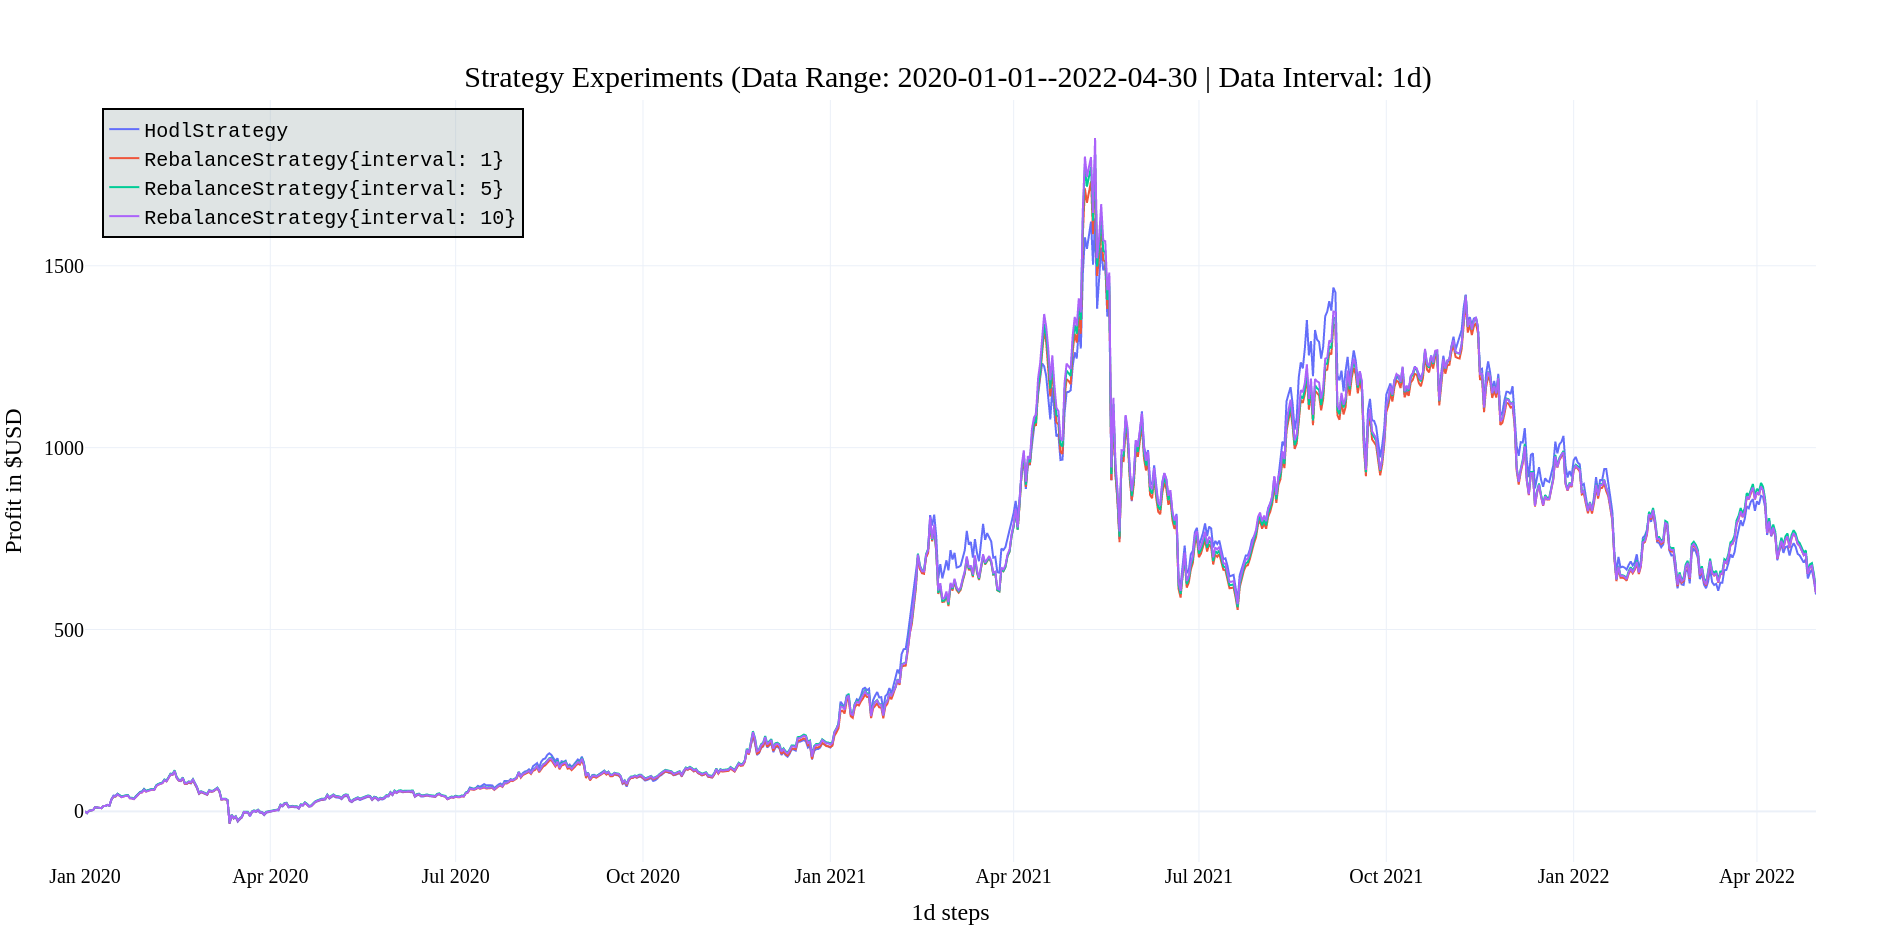
\includegraphics[width=\columnwidth]{figures/benchmark-B.png}
    \caption{Portfolio B: HODL and Rebalance performance}
    \label{figure-benchmark-2}
\end{figure}

\section{Implementation of Strategies---Risk Metric}
\label{section-strategies}

Unfortunately, Benjamin Cowen does not have his risk metric calculation formula publicly available. In a past video~\cite{youtube:cowen-moving-average}, he hinted that one piece used are the moving averages. Specifically when you take 50 day MA and you divide it by 50 week MA. That is the first value used.

\subsection*{Testing Out the 50 Week / 50 Days}
\label{subsection-50week50days}
The formula becomes:
$$risk = \frac{\mathit{SMA}_{50 days}}{\mathit{SMA}_{50 weeks}}$$

The results look quite similar to the metrics used by Benjamin Cowen. So far it is quite the approximation, but it seems to work nicely. For the reasons of the thesis colorcoded graph has been implemented. It shows the value of Bitcoin in time with colorbar on top of it---the more redder it is, the higher the risk, and vice versa.

Here are the results projected on historical price of Bitcoin. Results are shown in Figures \ref{figure-50week-scale} and \ref{figure-50week-colorcoded} as 0-1 scale and colorcoded graph respectively. As can be seen, the metric's beginning does not make much sense. It does well during the December 2017 peak. During the later peaks it performs okay, but the risk is not as high as it should be during the peak of April 2021. This tells us that we should not only look at the overall risk, but probably also at how quickly the risk changes.

\begin{figure}[!hbt]
    \centering
    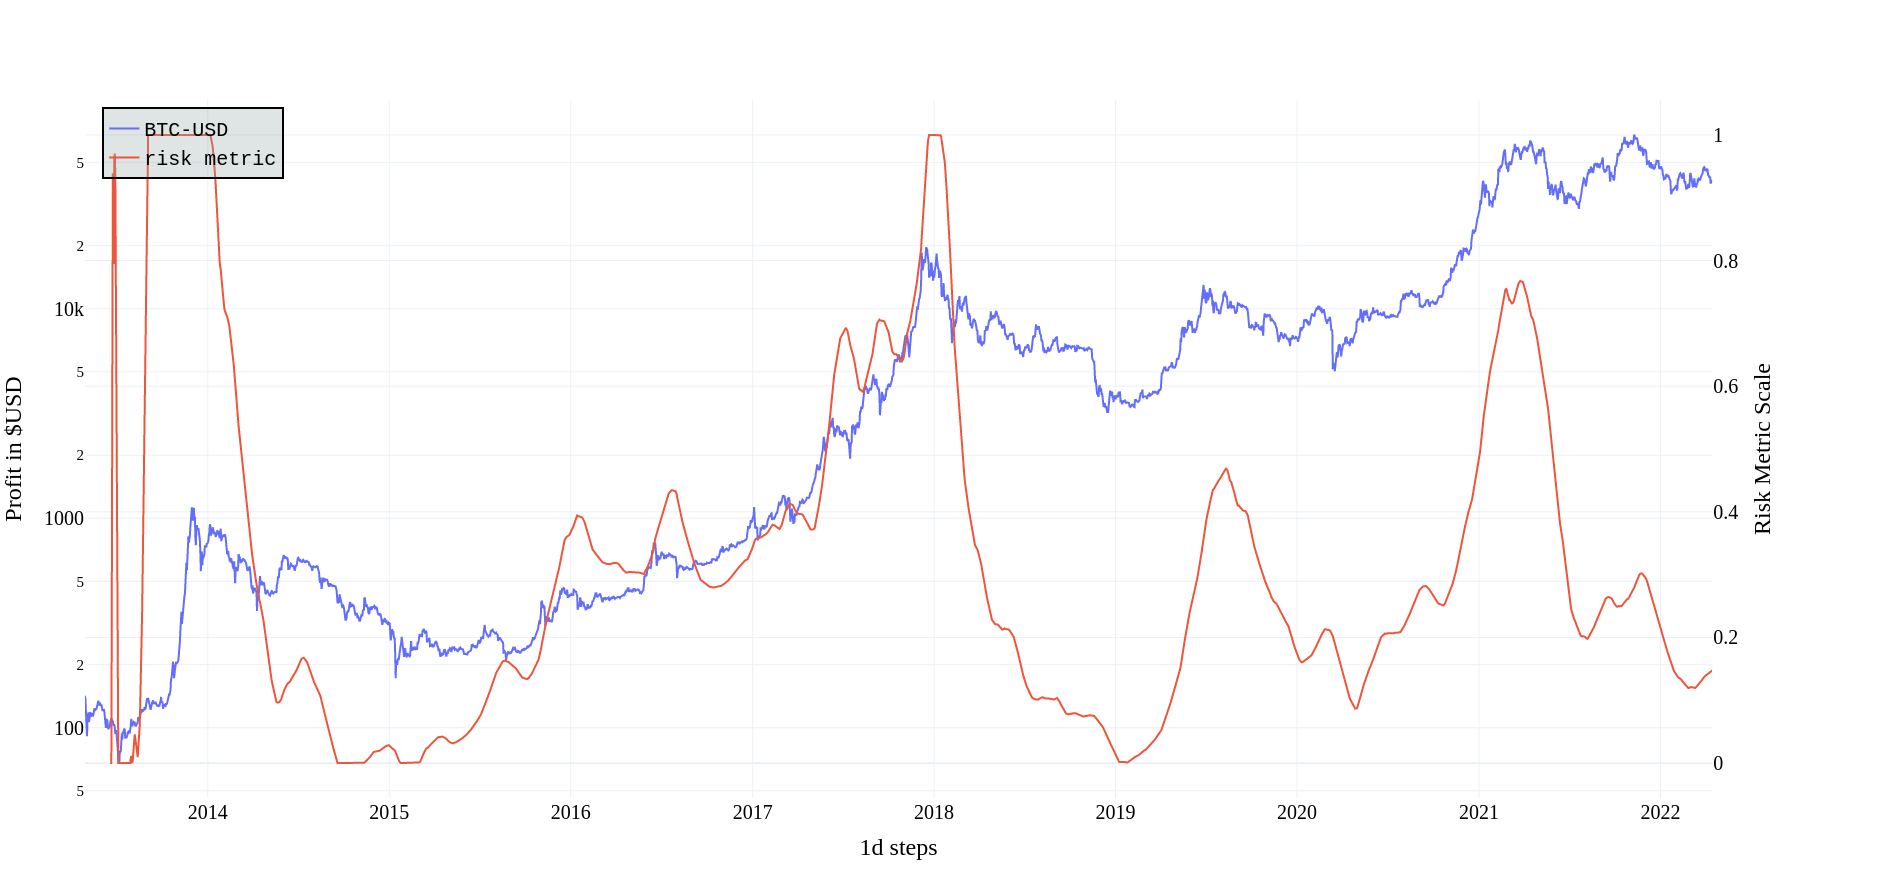
\includegraphics[width=\columnwidth]{figures/50week-scale.png}
    \caption{Historical Price of Bitcoin with Risk Metric Scale}
    \label{figure-50week-scale}
\end{figure}

\begin{figure}[!hbt]
    \centering
    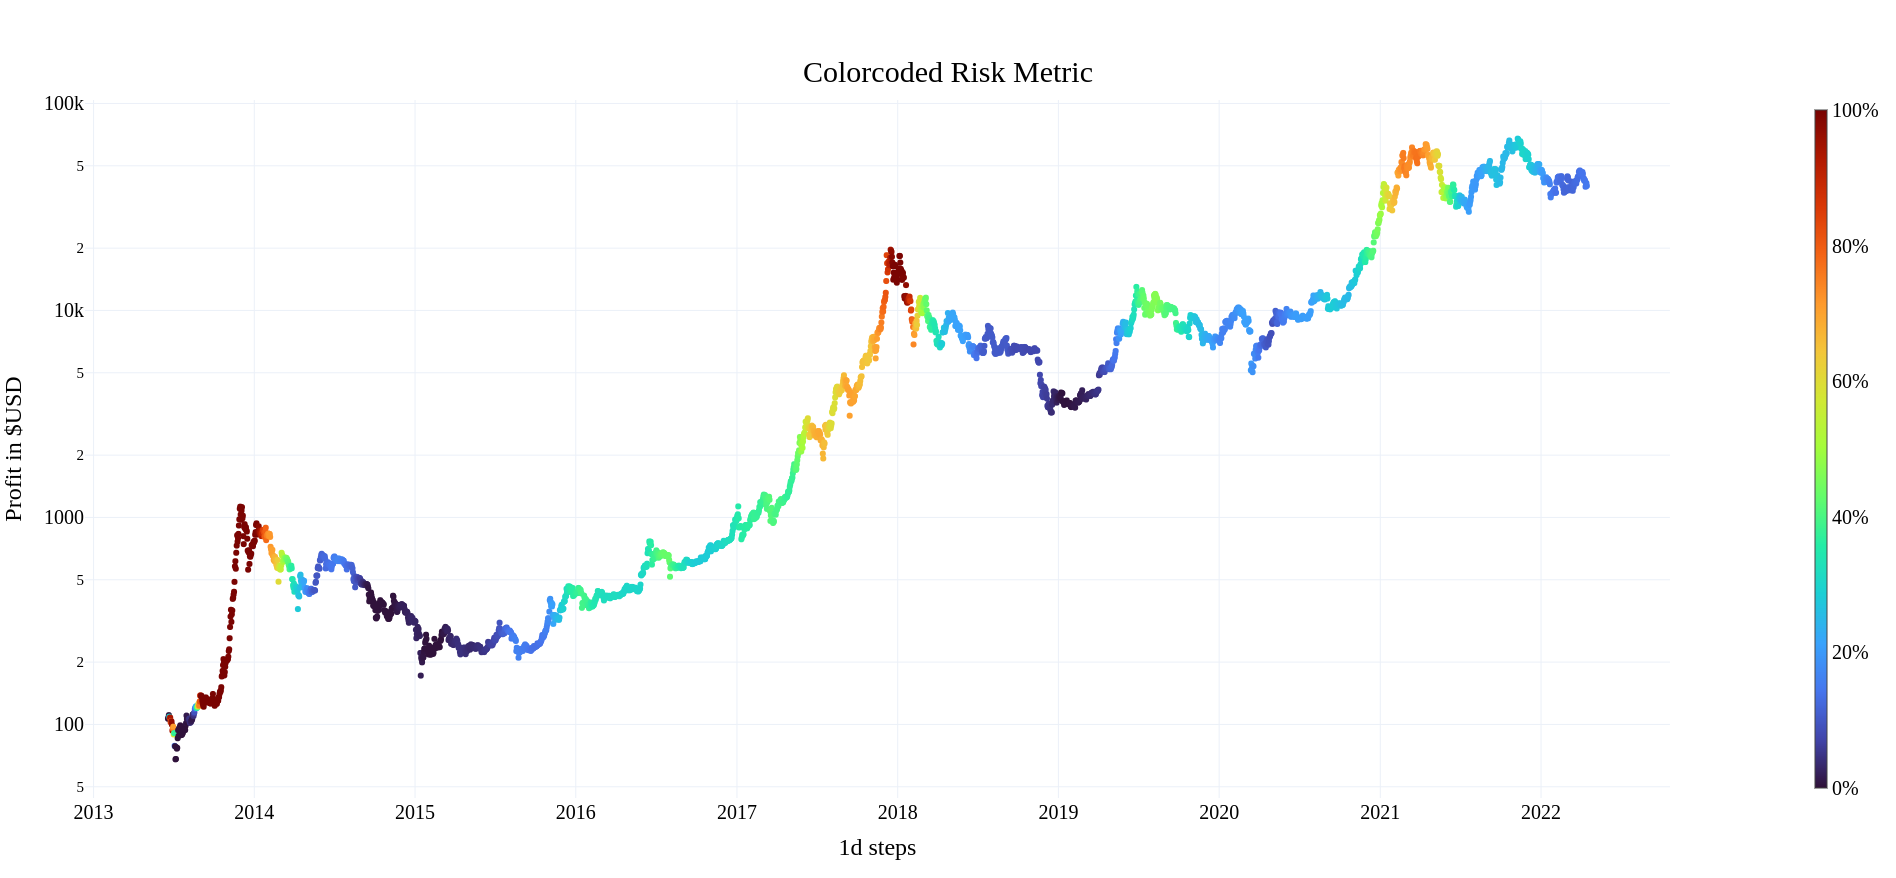
\includegraphics[width=\columnwidth]{figures/50week-colorcoded.png}
    \caption{Colorcoded Risk Metric}
    \label{figure-50week-colorcoded}
\end{figure}

\subsection*{Optimizing for Diminishing Returns}
\label{subsection-dimreturns}
What are diminishing returns? It is a theory in economics that predicts that after an optimal capacity level is reached, adding additional factor of production will result in smaller increase in output~\cite{investopedia:diminishing-returns}.

When we apply to Bitcoin, it means that the price growth is slowing, its returns are diminishing over time. Its supported by the fact that moving the price from 0.1\$ to 1\$ was relatively easy, but moving the price from 1000\$ to 10000\$ was significantly more difficult, requiring much more capital, even though the relative profit in percentages stays the same~\cite{bitcoin-diminishing-returns}. This would imply that expected returns of all hodlers diminish every time, making shorter-term hodlers more promising. This paragraph has been inspired by the source~\cite{bitcoin-diminishing-returns}.

Formula used by the diminishing returns has been inspired by this article~\cite{bitcoin-diminishing-returns-formula}. General formula used:
$$price = 10^{(a + b \log_{10}(d))}$$

with a = -17.01593313 and the slope b = 5.84509376 with d the number of days since 2009 Jan 12, first ever recorded Bitcoin exchange.

Expected price of Bitcoin, according to the formula above, can be seen in Figure \ref{figure-dim-formula}. The formula tells us that we should optimize for diminishing returns, but not only that. The equation itself can be used to serve as a metric. If the price is above the expected threshold, the investor should be cautious. When it is below, the investor can act more bullishly.

\begin{figure}[!hbt]
    \centering
    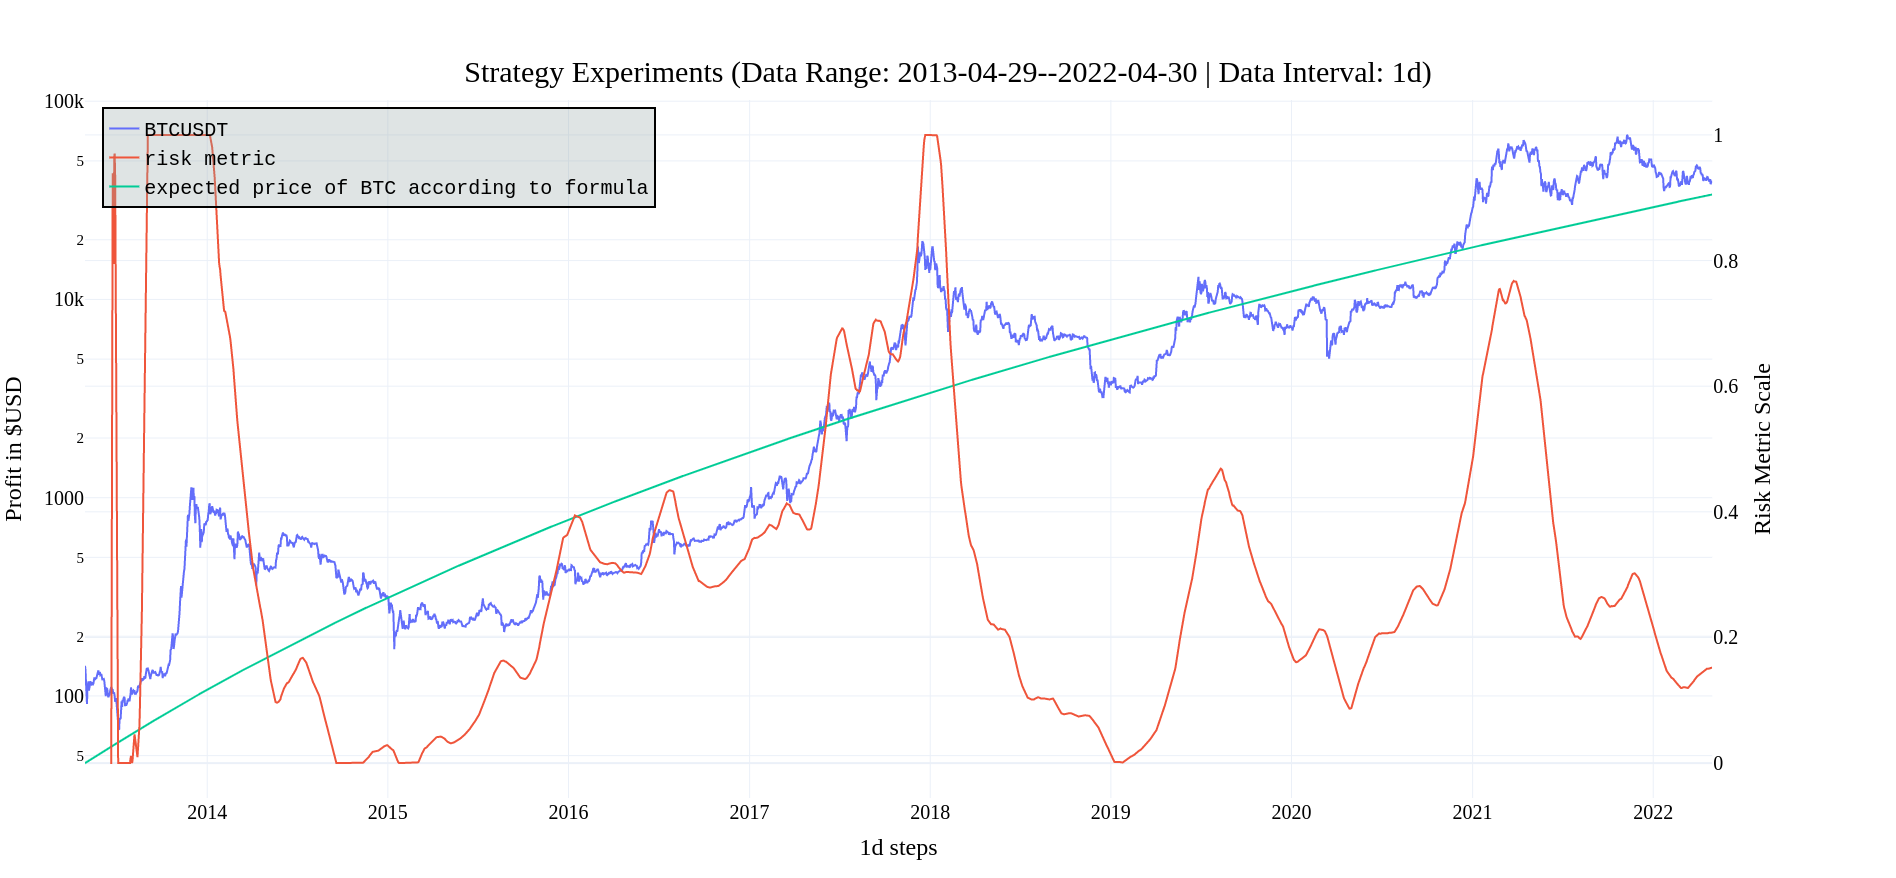
\includegraphics[width=\columnwidth]{figures/expected-price-formula.png}
    \caption{Expected price of Bitcoin according to diminishing returns formula.}
    \label{figure-dim-formula}
\end{figure}


For now, let us only optimize the risk metric we have so far implemented. Optimizing for diminishing returns in this sense means that the risk should be higher for the later dates, even though the moving averages have the same values. The result of moving averages will be multiplied by some constant that is computed by the number of days that have passed since the year 2009. The previous formula becomes:

$$risk = \frac{\mathit{SMA}_{50 days}}{\mathit{SMA}_{50 weeks}} * \log_{10}(d)$$

The $\log$ part could be further tweaked with, but I have found that it works quite nicely. In Figure \ref{figure-dim-riskmetric} you can see the optimized risk metric against the original.

\begin{figure}[!hbt]
    \centering
    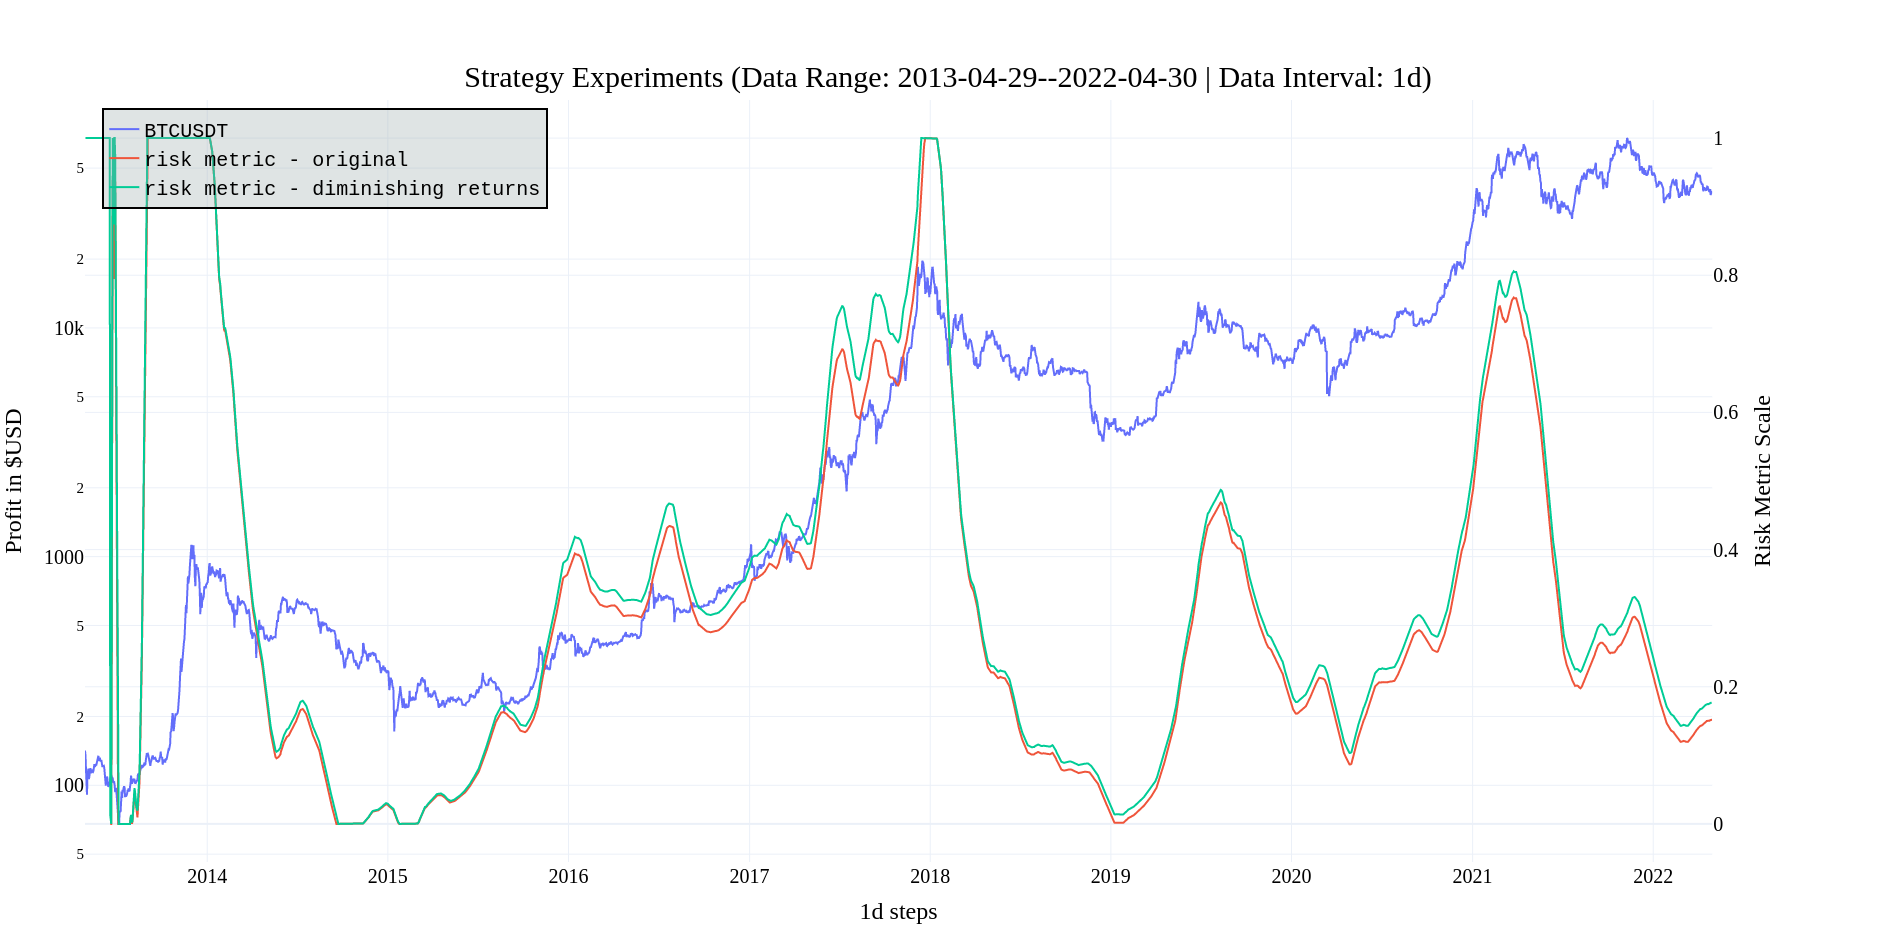
\includegraphics[width=\columnwidth]{figures/riskmetric-dim-returns.png}
    \caption{Comparison of the diminishing returns optimization against the original.}
    \label{figure-dim-riskmetric}
\end{figure}

\subsection*{Using Total Market Capitalization Data}
\label{subsection-marketcap}
Other thing considered is using the total market capitalization data instead of the historical price for bitcoin. This metric makes sense when using more types of cryptocurrencies than just bitcoin. All calculations and formulas stay the same, the only that changes is the data used---switching bitcoin data for total market capitalization.

In Figures \ref{figure-total-marketcap-riskmetric} and \ref{figure-total-marketcap-riskmetric-dim-returns} comparison to the previous findings with the bitcoin risk metric can be seen. The metrics are quite similar, the bigger difference is that the total market capitalization metric gives more importance to the jump of July 2017. The diminishing returns optimization optimze the metrics, but no other change is observed.

\begin{figure}[!hbt]
    \centering
    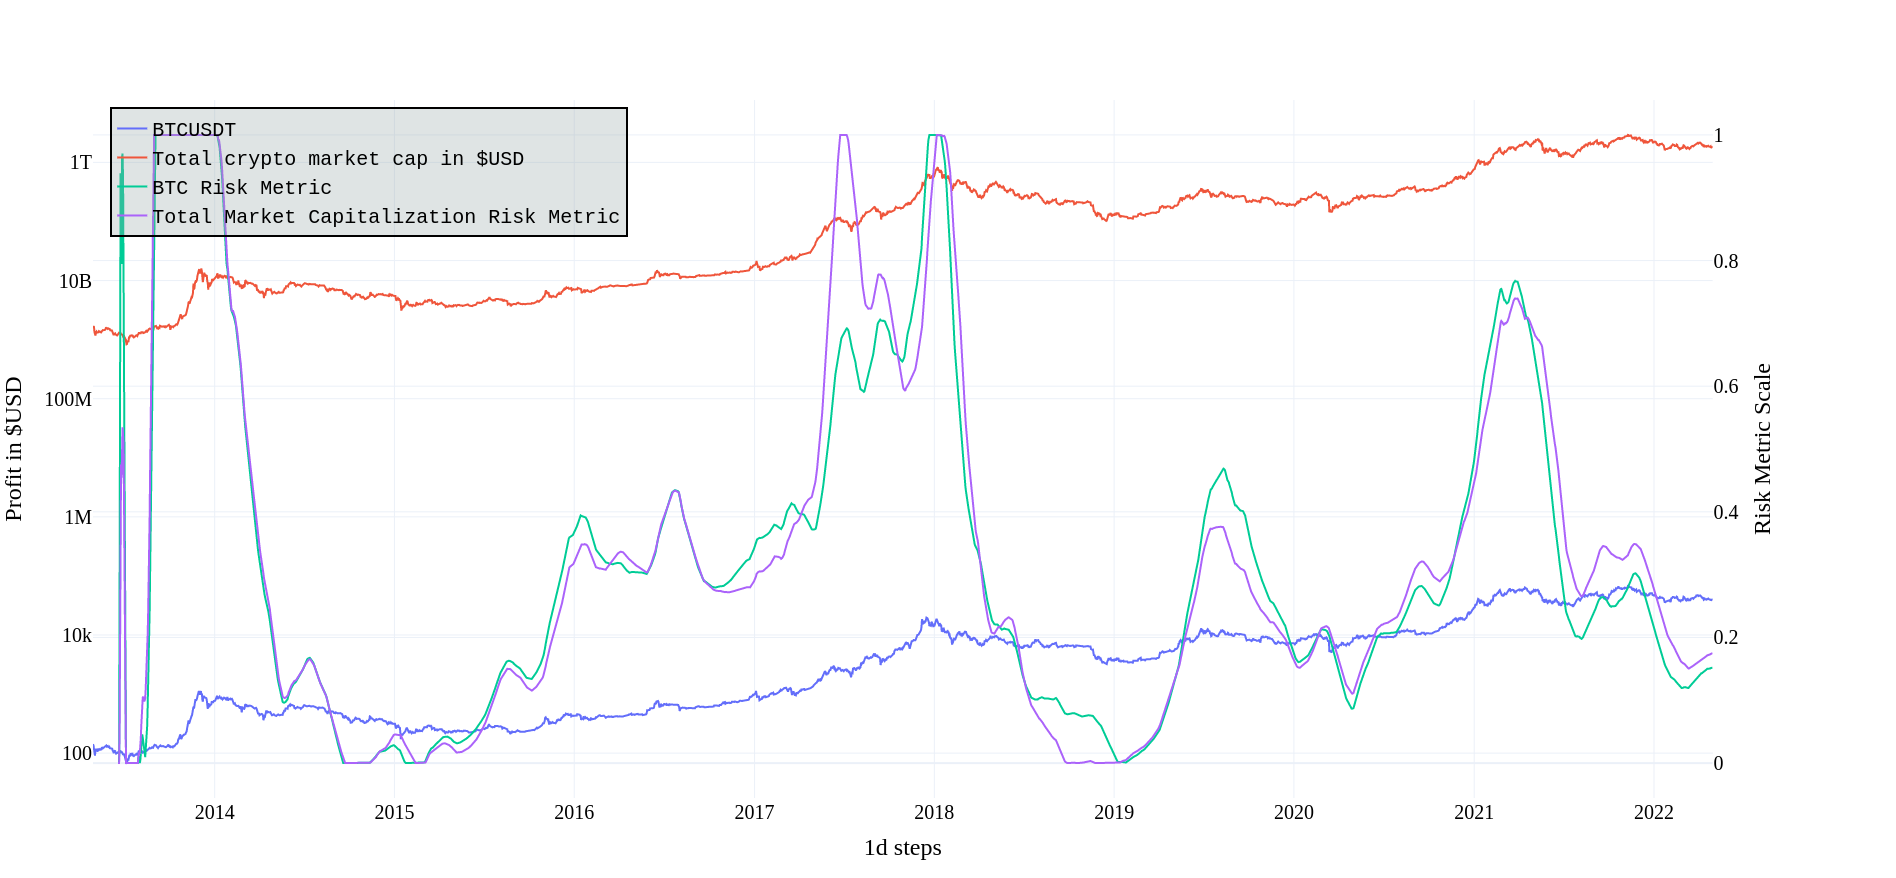
\includegraphics[width=\columnwidth]{figures/totalmarketcap-metric.png}
    \caption{Comparison of bitcoin data usage against total market capitalization data for the risk metric.}
    \label{figure-total-marketcap-riskmetric}
\end{figure}

\begin{figure}[!hbt]
    \centering
    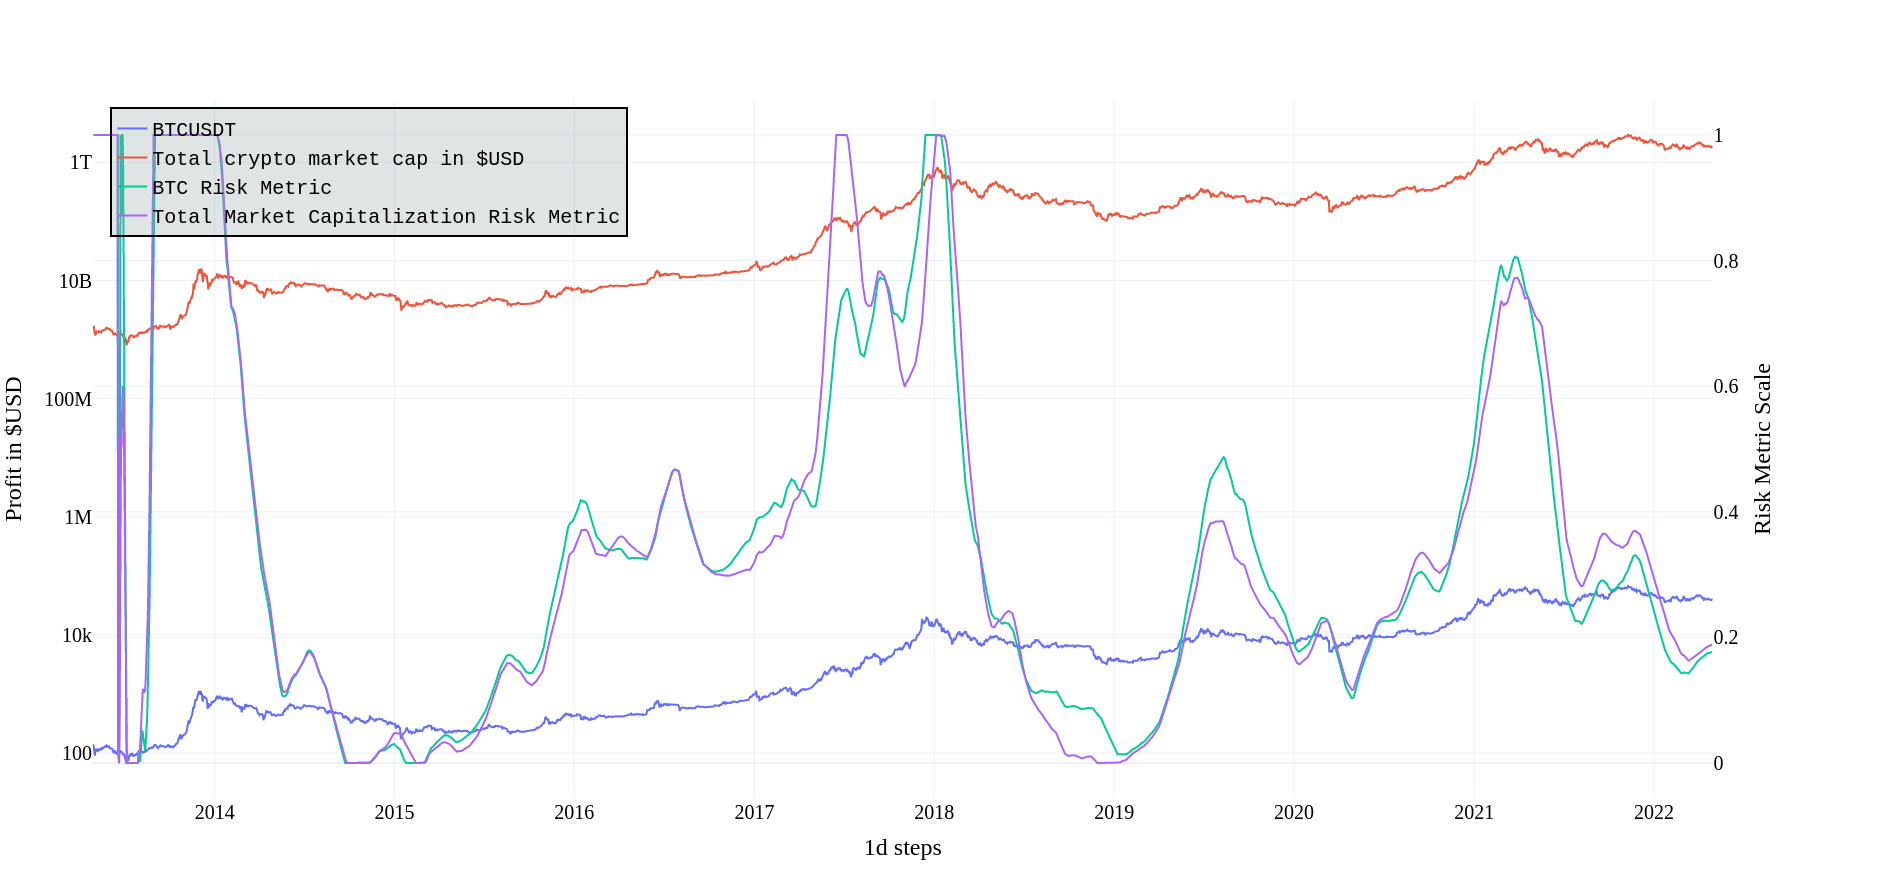
\includegraphics[width=\columnwidth]{figures/totalmarketcap-metric-dimreturns.png}
    \caption{Comparison of bitcoin data usage against total market capitalization data for the risk metric. Diminishing returns optimization is applied.}
    \label{figure-total-marketcap-riskmetric-dim-returns}
\end{figure}

\subsection*{Correlation With 24h Volume Data}
\label{subsection-24hvolume-correlation}
When using a strategy like the risk metric we have implemented, we are betting on one horse so to speak. Some unexpected turn can make us lose a lot of money. That is why it is sometimes more efficient to use a correlation with a different strategy to make the original strategy less error-prone. That is the motivation for this seciton.

Correlation with the volume in \$USD traded in one day has been chosen for our strategy. It is a sensible metric. When more people trade the asset the price can be expected to fluctuate a lot---usually up---and vice versa.

The data correlation between the two series is approximately $0.73$, with $1$ being the best positive correlation. The computed correlation is not perfect, but it gives us a good basis to work upon. Comparison can be seen in Figures \ref{figure-24volume-ols}, \ref{figure-24volume-lin} and \ref{figure-24volume-log}.

\begin{figure}[!hbt]
    \centering
    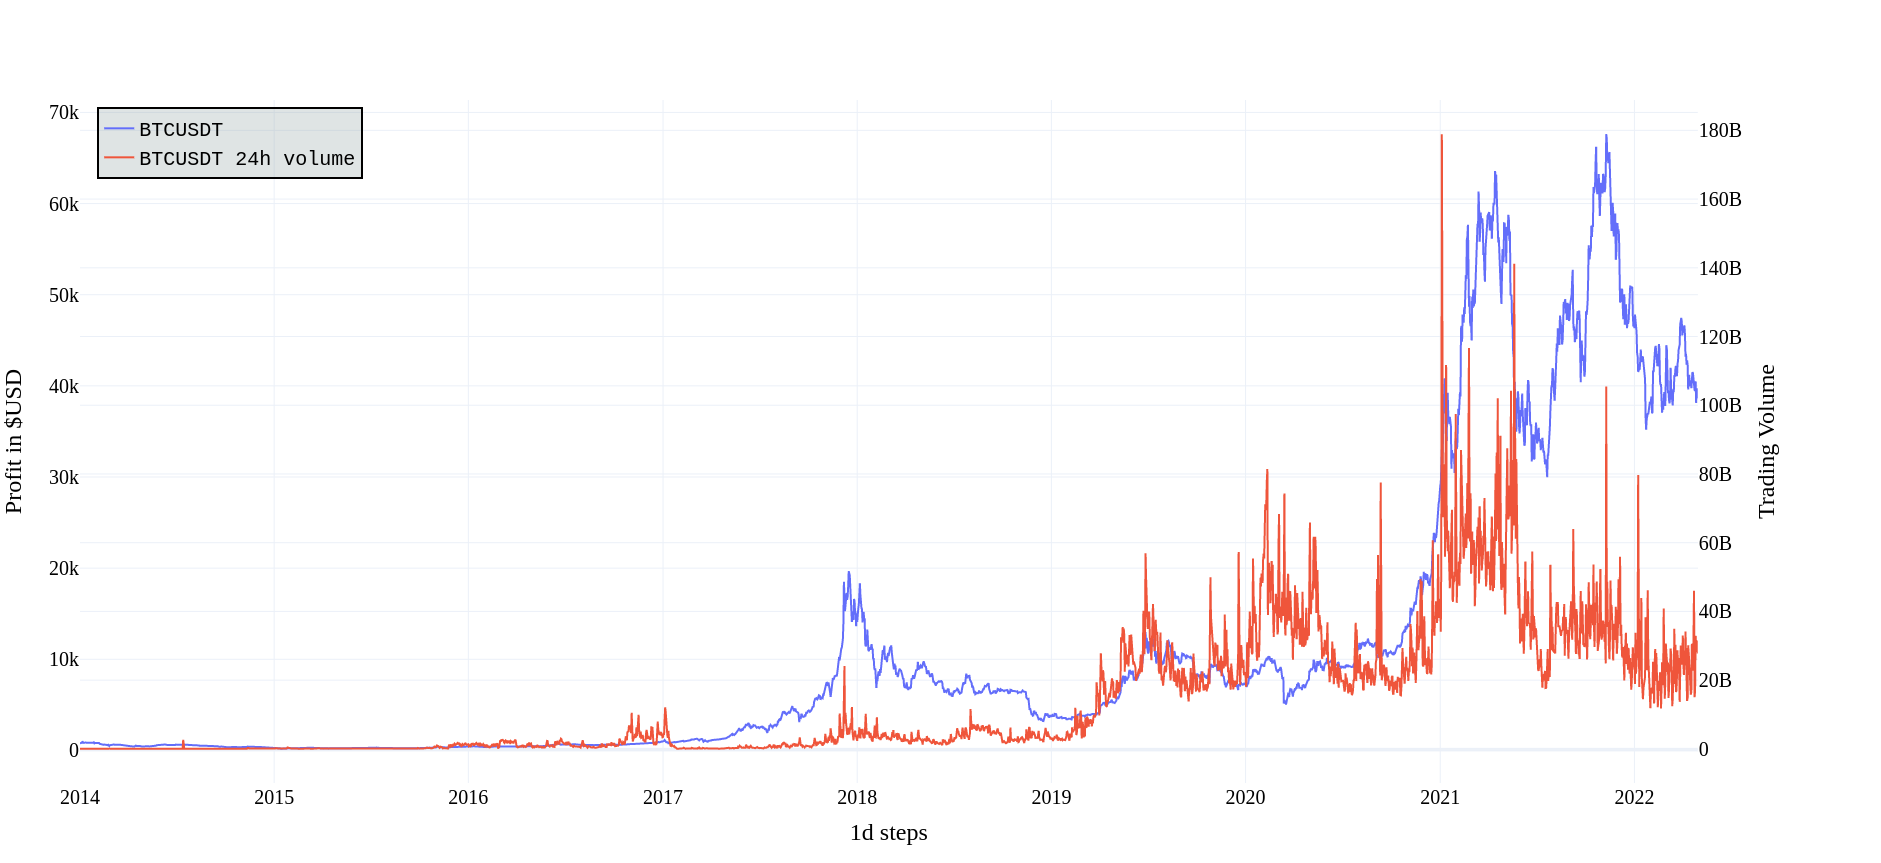
\includegraphics[width=\columnwidth]{figures/24volume-ols.png}
    \caption{Ordinary Least Squares method~\cite{wikipedia:ols} visualizing the correlation.}
    \label{figure-24volume-ols}
\end{figure}

\begin{figure}[!hbt]
    \centering
    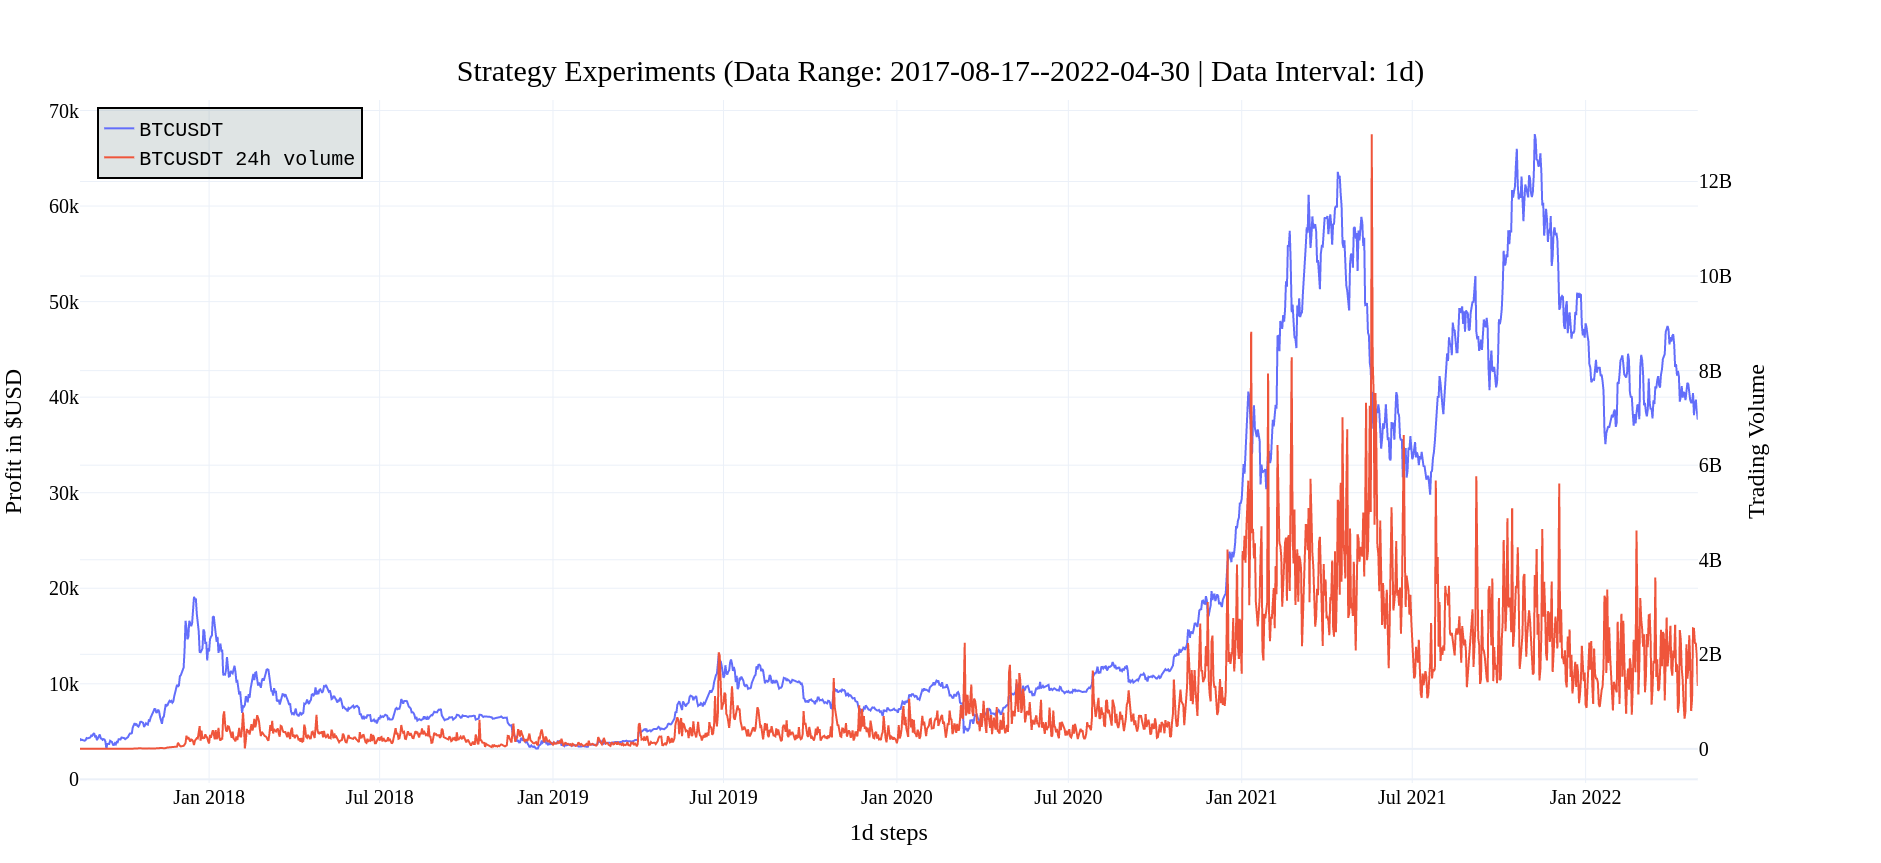
\includegraphics[width=\columnwidth]{figures/24volume-lin.png}
    \caption{Linear graph comparison between Bitcoin price and \$USD volume.}
    \label{figure-24volume-lin}
\end{figure}

\begin{figure}[!hbt]
    \centering
    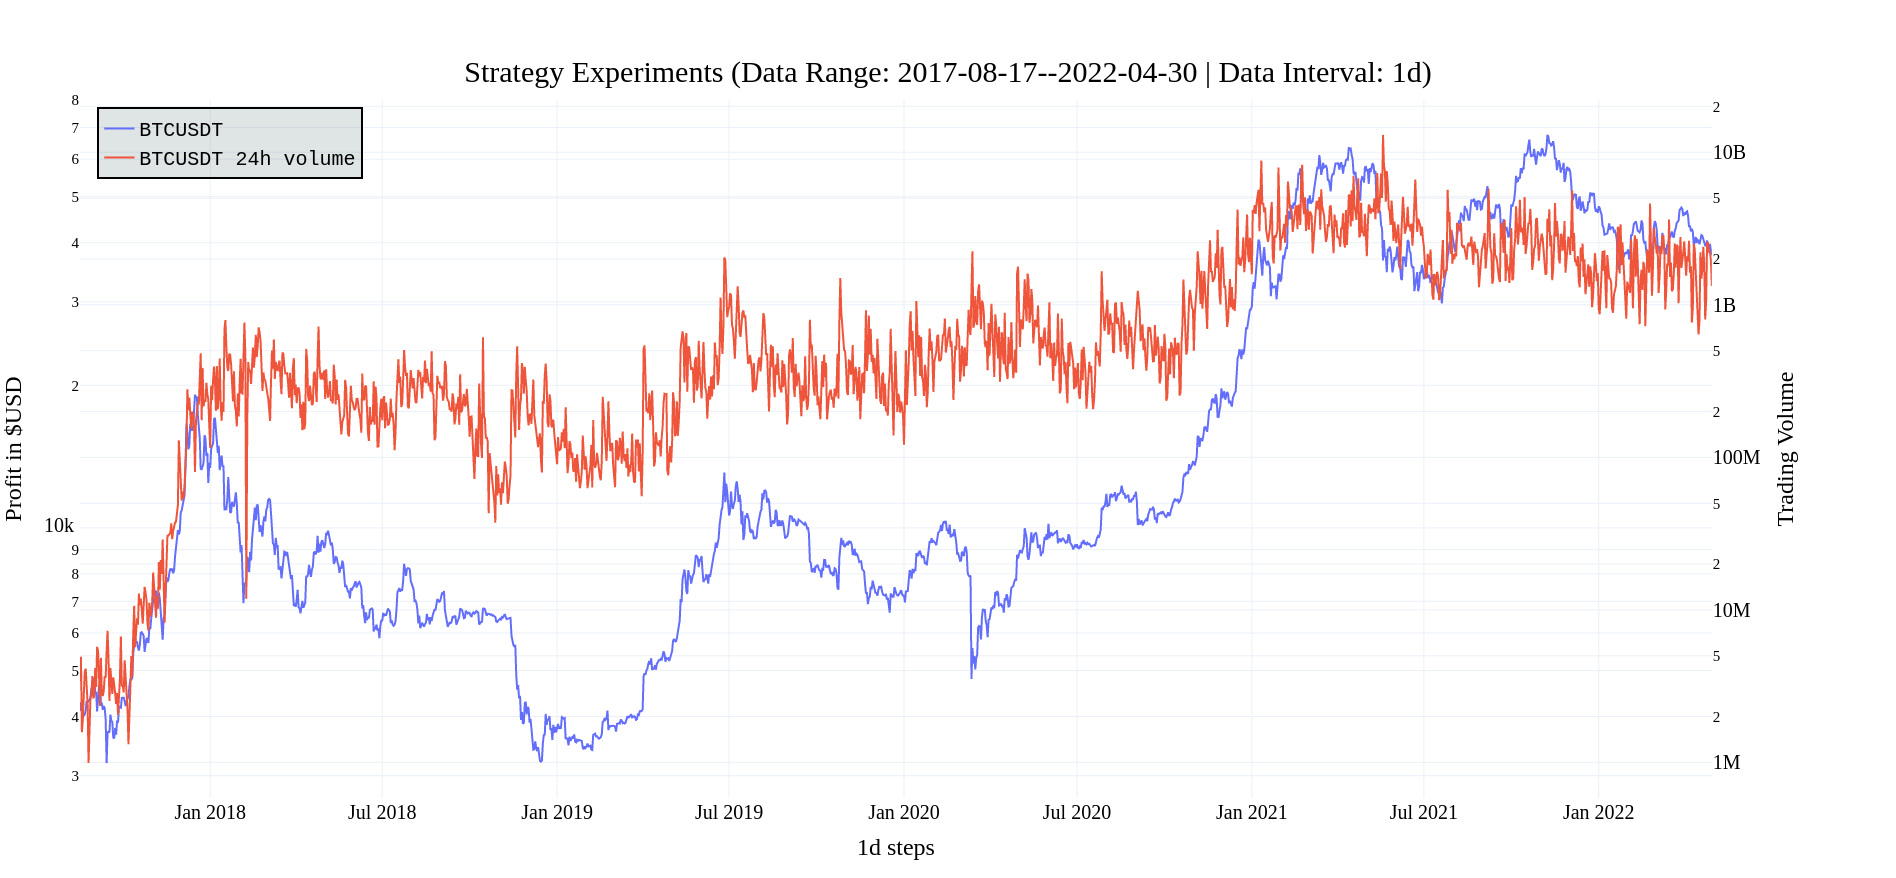
\includegraphics[width=\columnwidth]{figures/24volume-log.png}
    \caption{Log-log graph comparing the Bitcoin price and its \$USD volume.}
    \label{figure-24volume-log}
\end{figure}

Next step is to incorporate the daily \$USD volume with the risk metric. There are two ways to go about it. Either we incorporate the daily trading volume directly into the risk metric, making the risk higher when more volume is traded and vice versa. Or we incorporate the daily trading volume into the evaluation strategy. That means we will decide the buy or sell not just by the risk metric, but the evaluation algorithm will take the daily trading volume into consideration, too.

Choosing the first approach, incorporating the trading volume into the risk metric itself, we can go about it in the following way. First we compute the smooth rolling average of the last 7 days of the trading volume. We take this average and normalize it between values 0.5 and -0.5. Then we take the original risk metric and we add some reduced value of the trading volume average on top of it, making the risk higher if more volume has been traded in the last 7 days and lower if less volume has been traded.

The following formula is produced, the $'$ sign represent the normalization between $0$--$1$. The symbols BTC\_SMA represents the bitcoin smooth moving average and VOL\_SMA represent the trading volume moving average. I found that the quoficient of $0.2$ works quite well.
$$risk = \left(\frac{\mathit{BTC\_SMA}_{50 days}}{\mathit{BTC\_SMA}_{50 weeks}}\right)' + \left(\mathit{VOL\_SMA}_{7 days}' - 0.5\right) * 0.2$$

When optimizing it for diminishing returns, we just alter the original metric:
$$risk = \left[\frac{\mathit{BTC\_SMA}_{50 days}}{\mathit{BTC\_SMA}_{50 weeks}} * \log_{10}(d)\right]' + \left(\mathit{VOL\_SMA}_{7 days}' - 0.5\right) * 0.2$$

In Figure \ref{figure-24volume-7sma} the 7 days moving average of trading volume can be seen. In Figures \ref{figure-24volume-riskmetric} and \ref{figure-24volume-riskmetric-dimreturns} there can be seen how the correlated risk metrics fare against the original metric. In the second figure, the metric is optimized for diminishing returns.

\begin{figure}[!hbt]
    \centering
    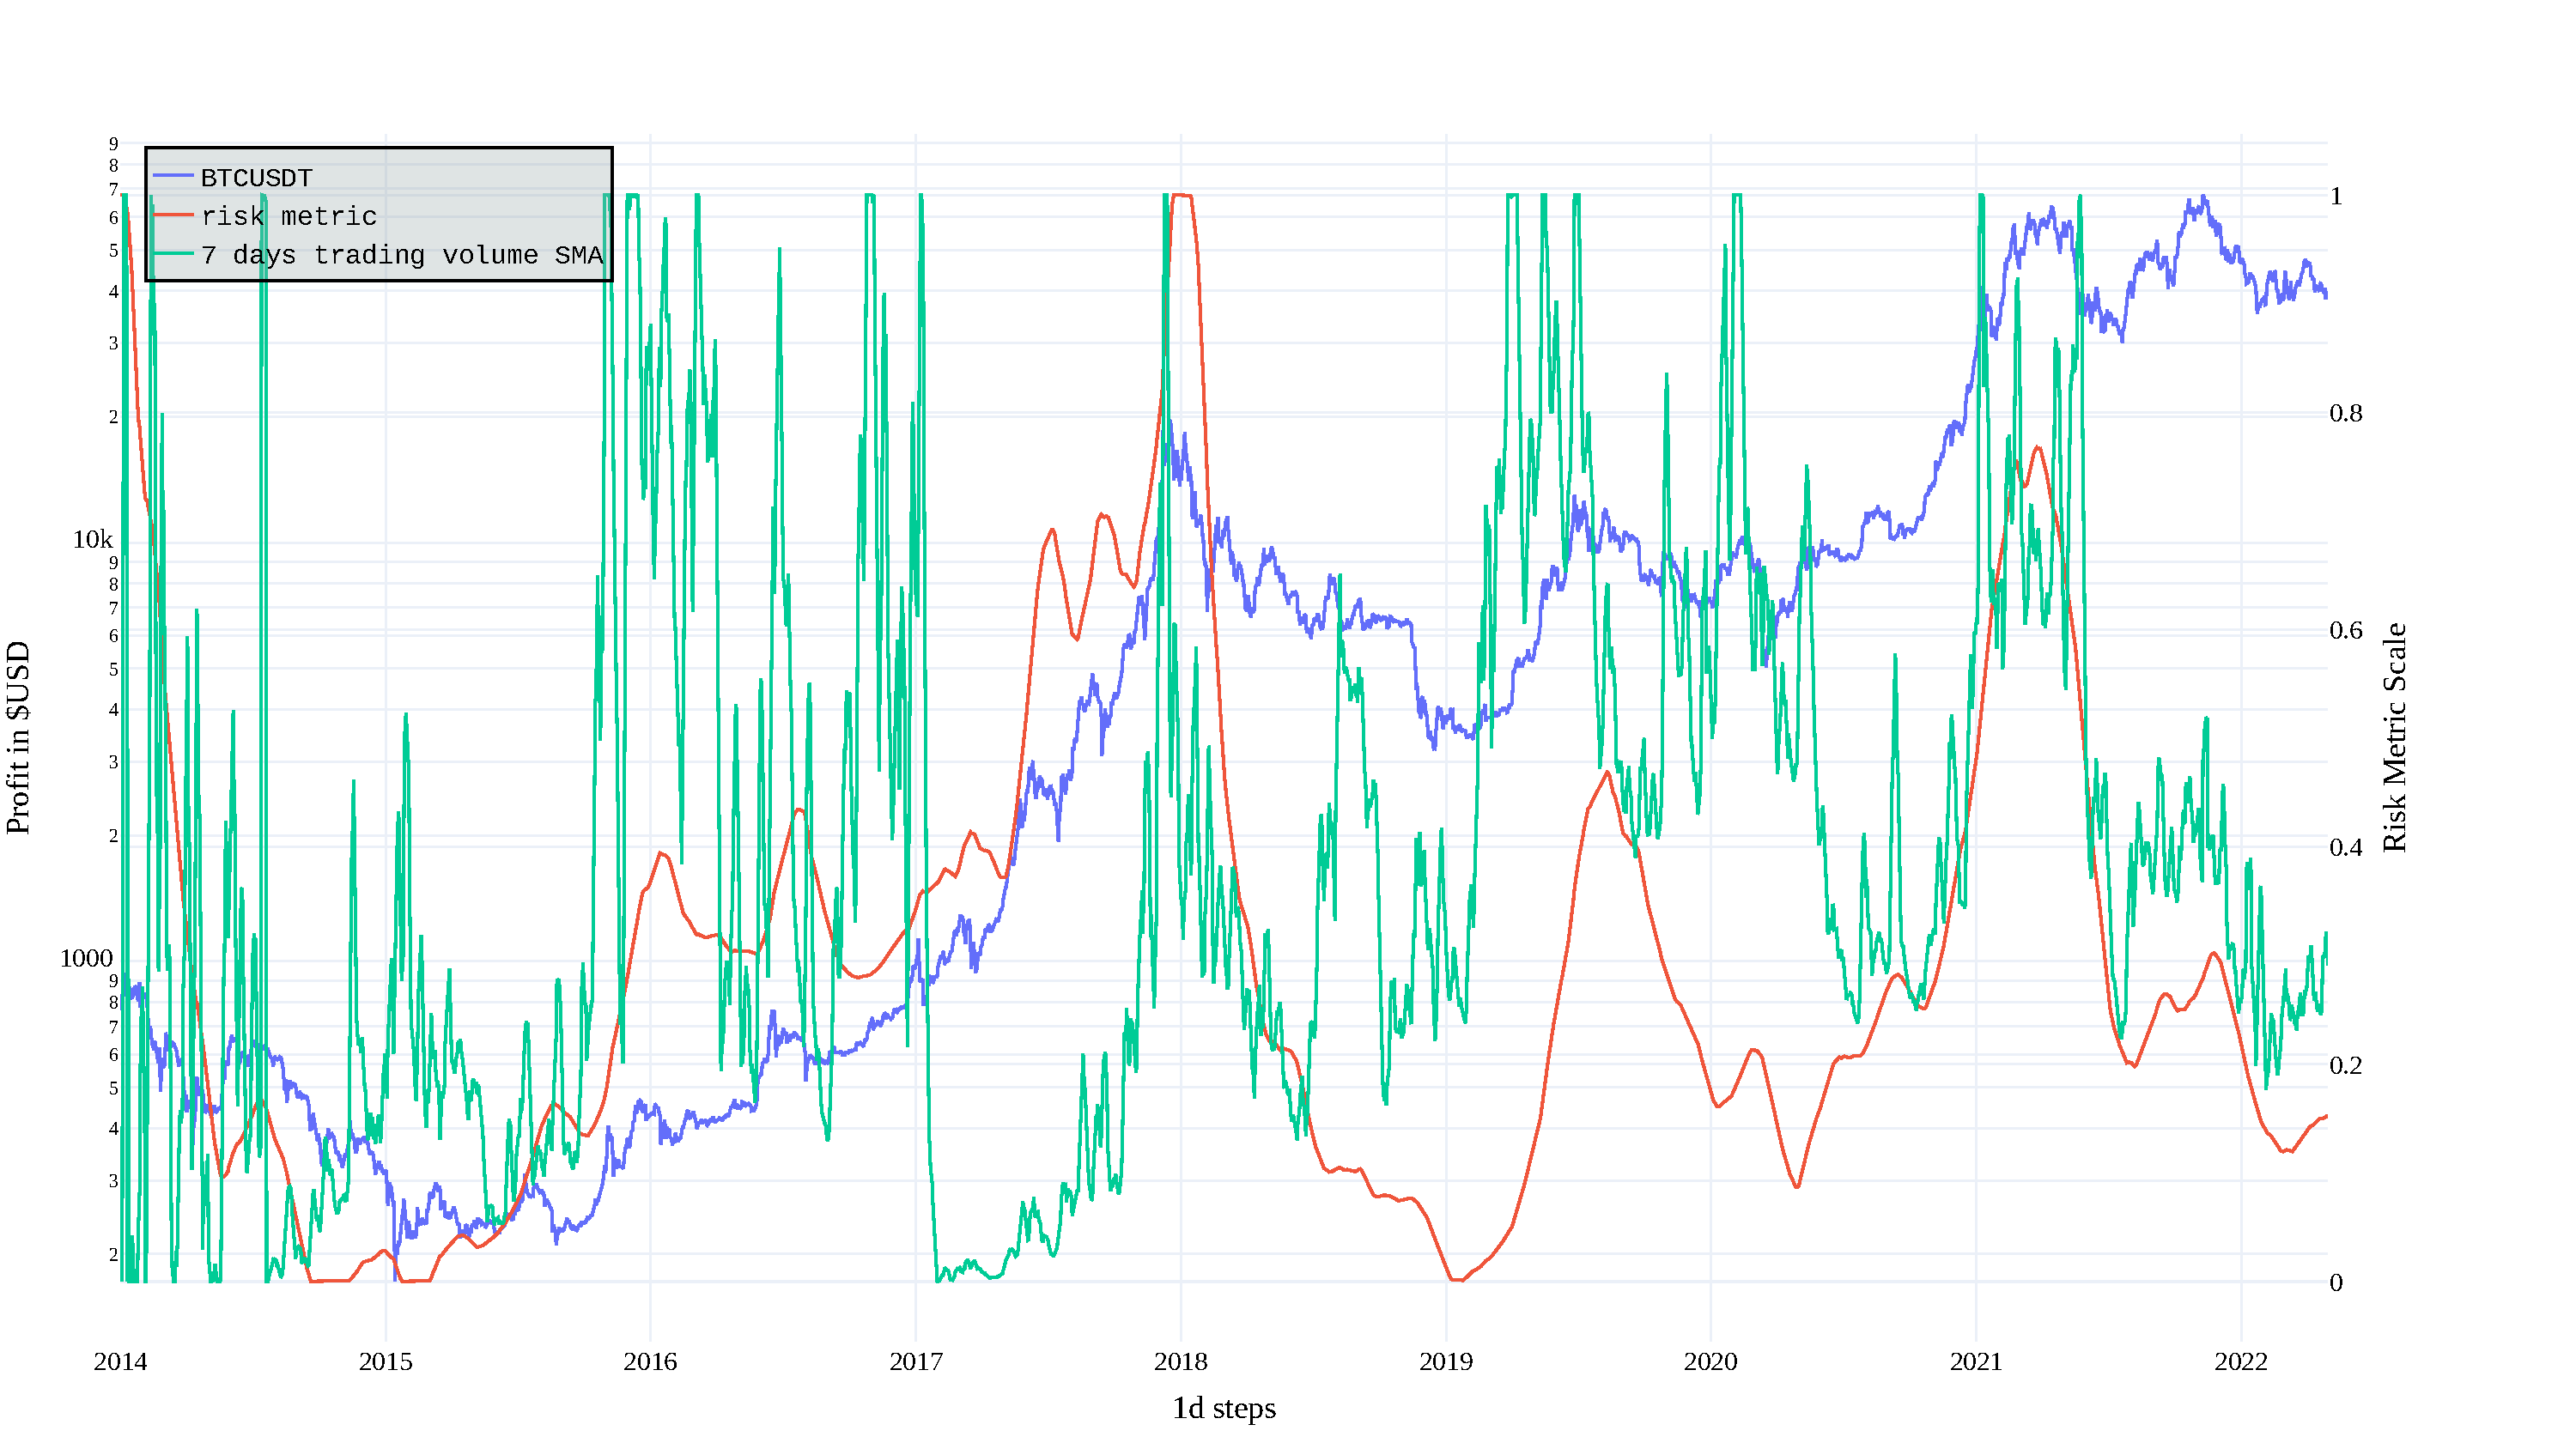
\includegraphics[width=\columnwidth]{figures/24volume-7sma.pdf}
    \caption{Ordinary Least Squares method~\cite{wikipedia:ols} visualizing the correlation.}
    \label{figure-24volume-7sma}
\end{figure}

\begin{figure}[!hbt]
    \centering
    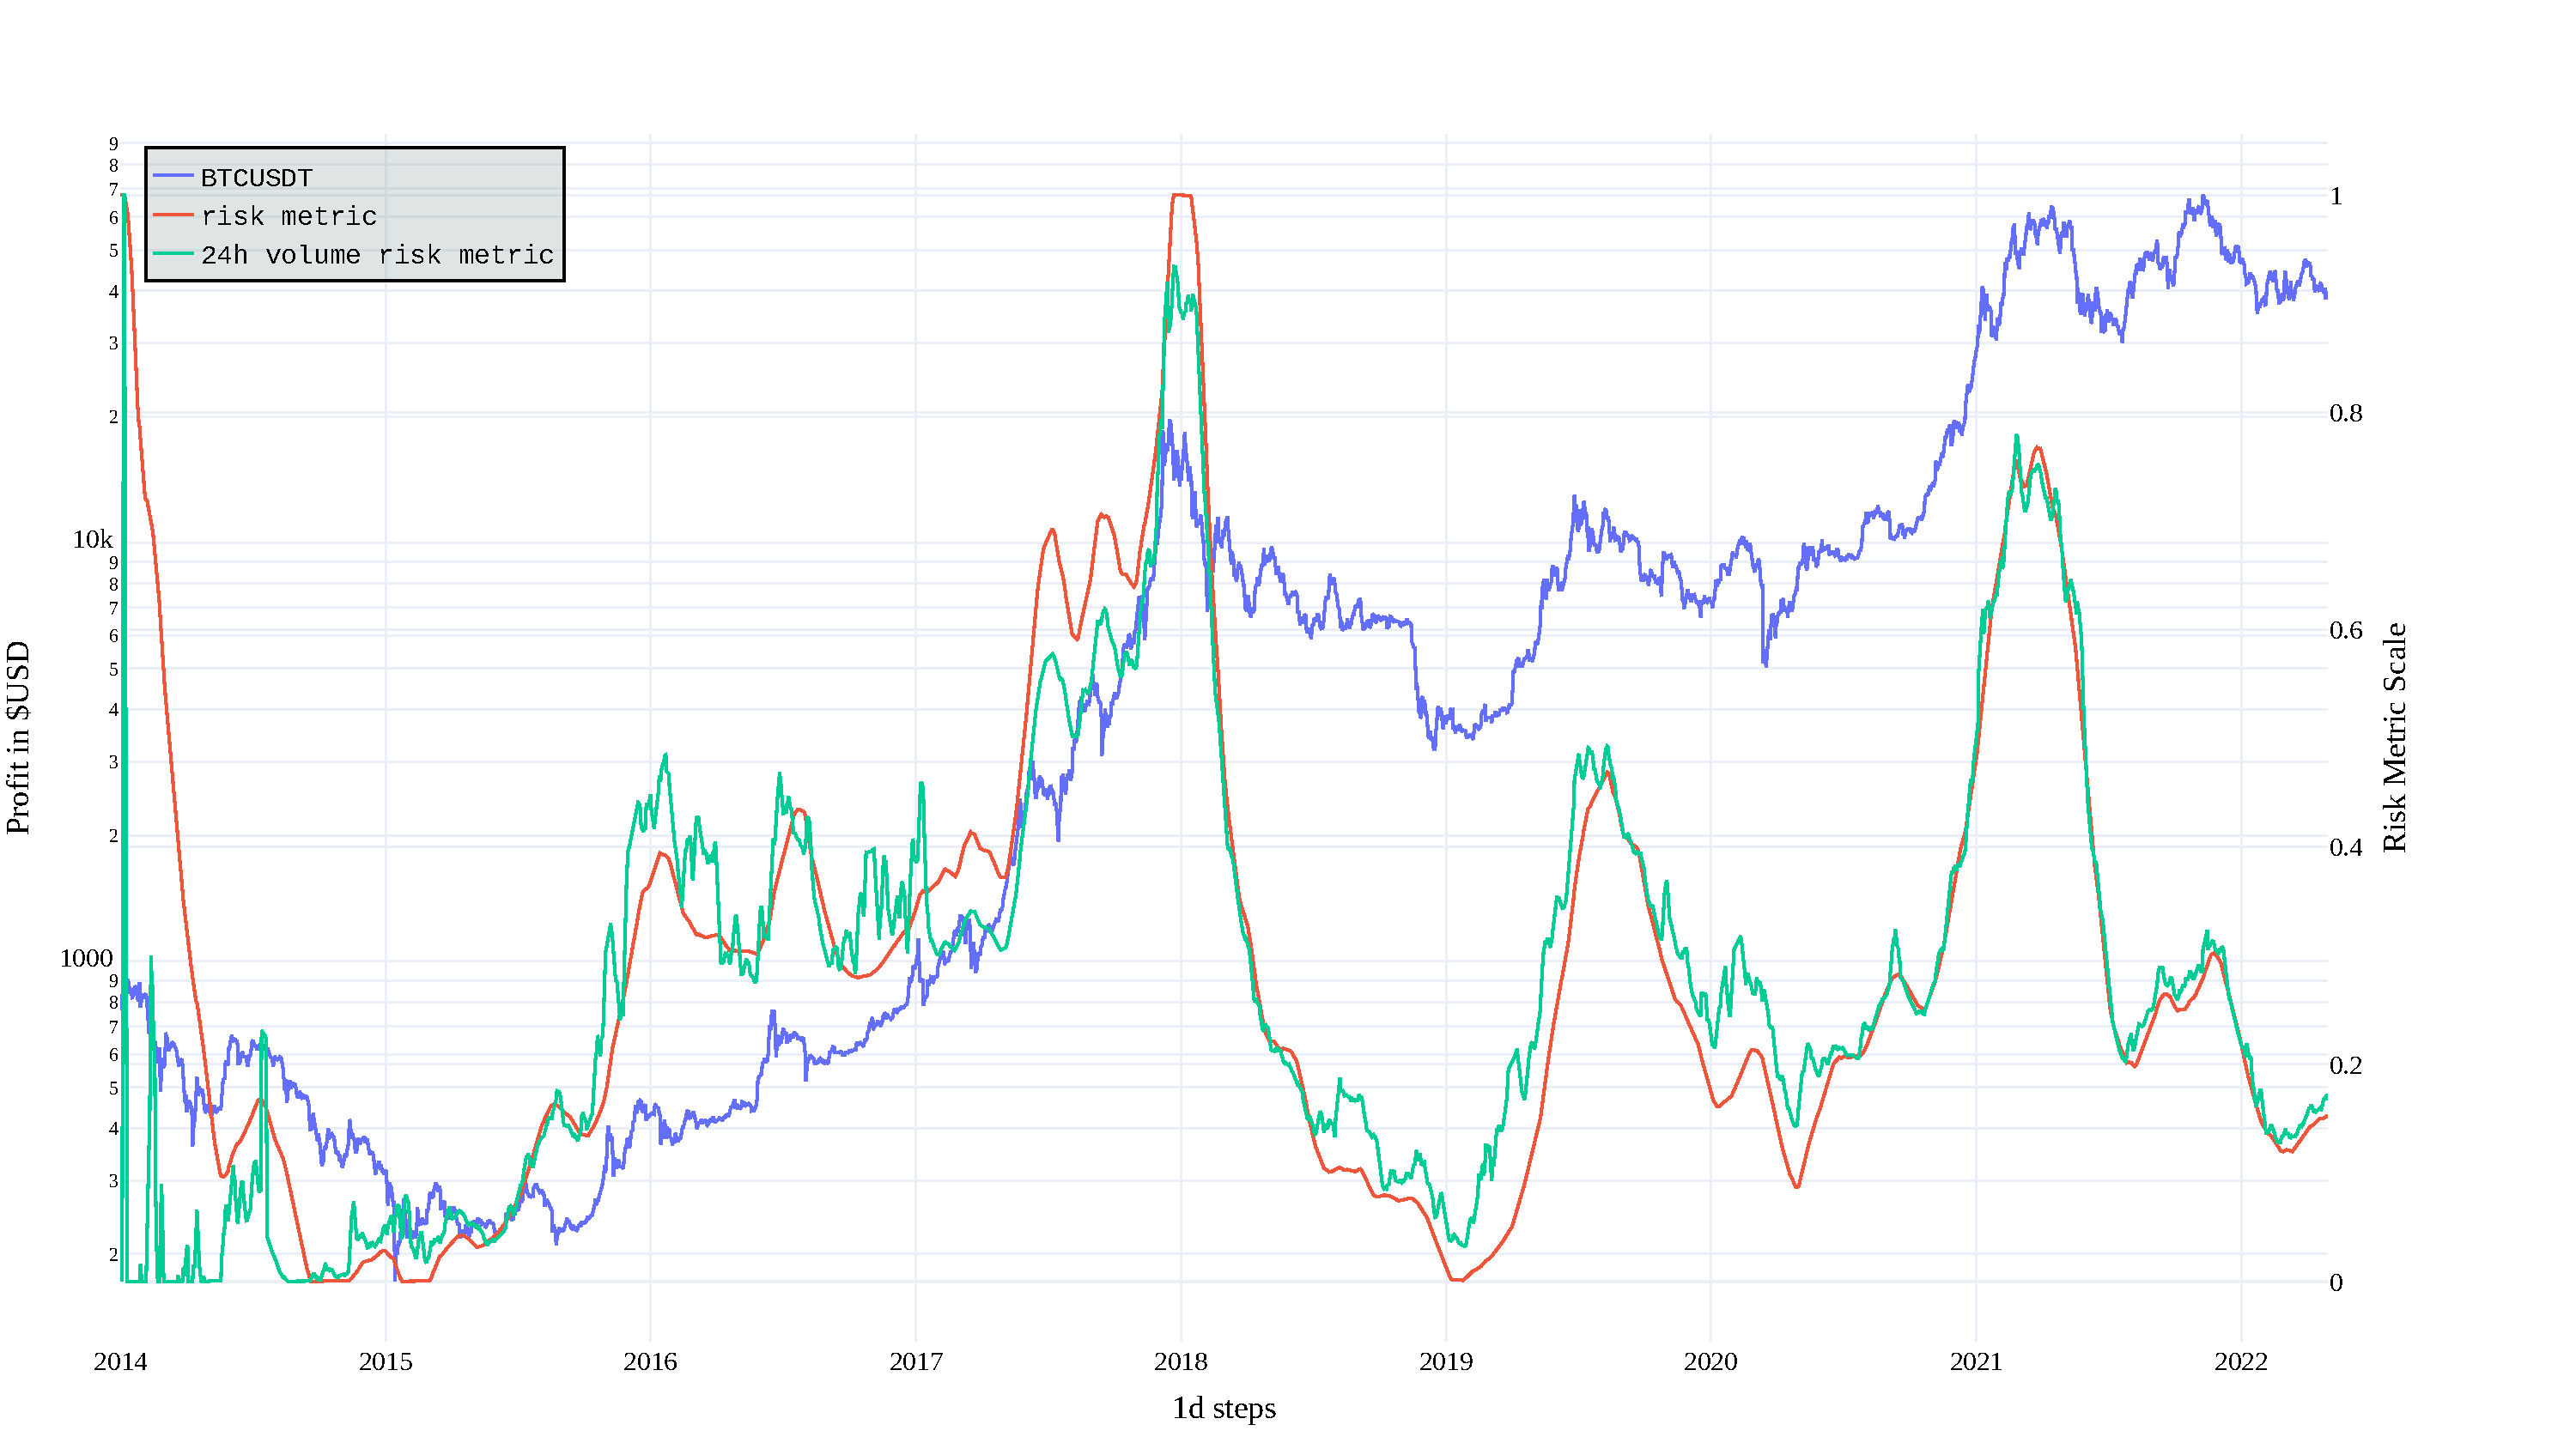
\includegraphics[width=\columnwidth]{figures/24volume-riskmetric.pdf}
    \caption{Linear graph comparison between Bitcoin price and \$USD volume.}
    \label{figure-24volume-riskmetric}
\end{figure}

\begin{figure}[!hbt]
    \centering
    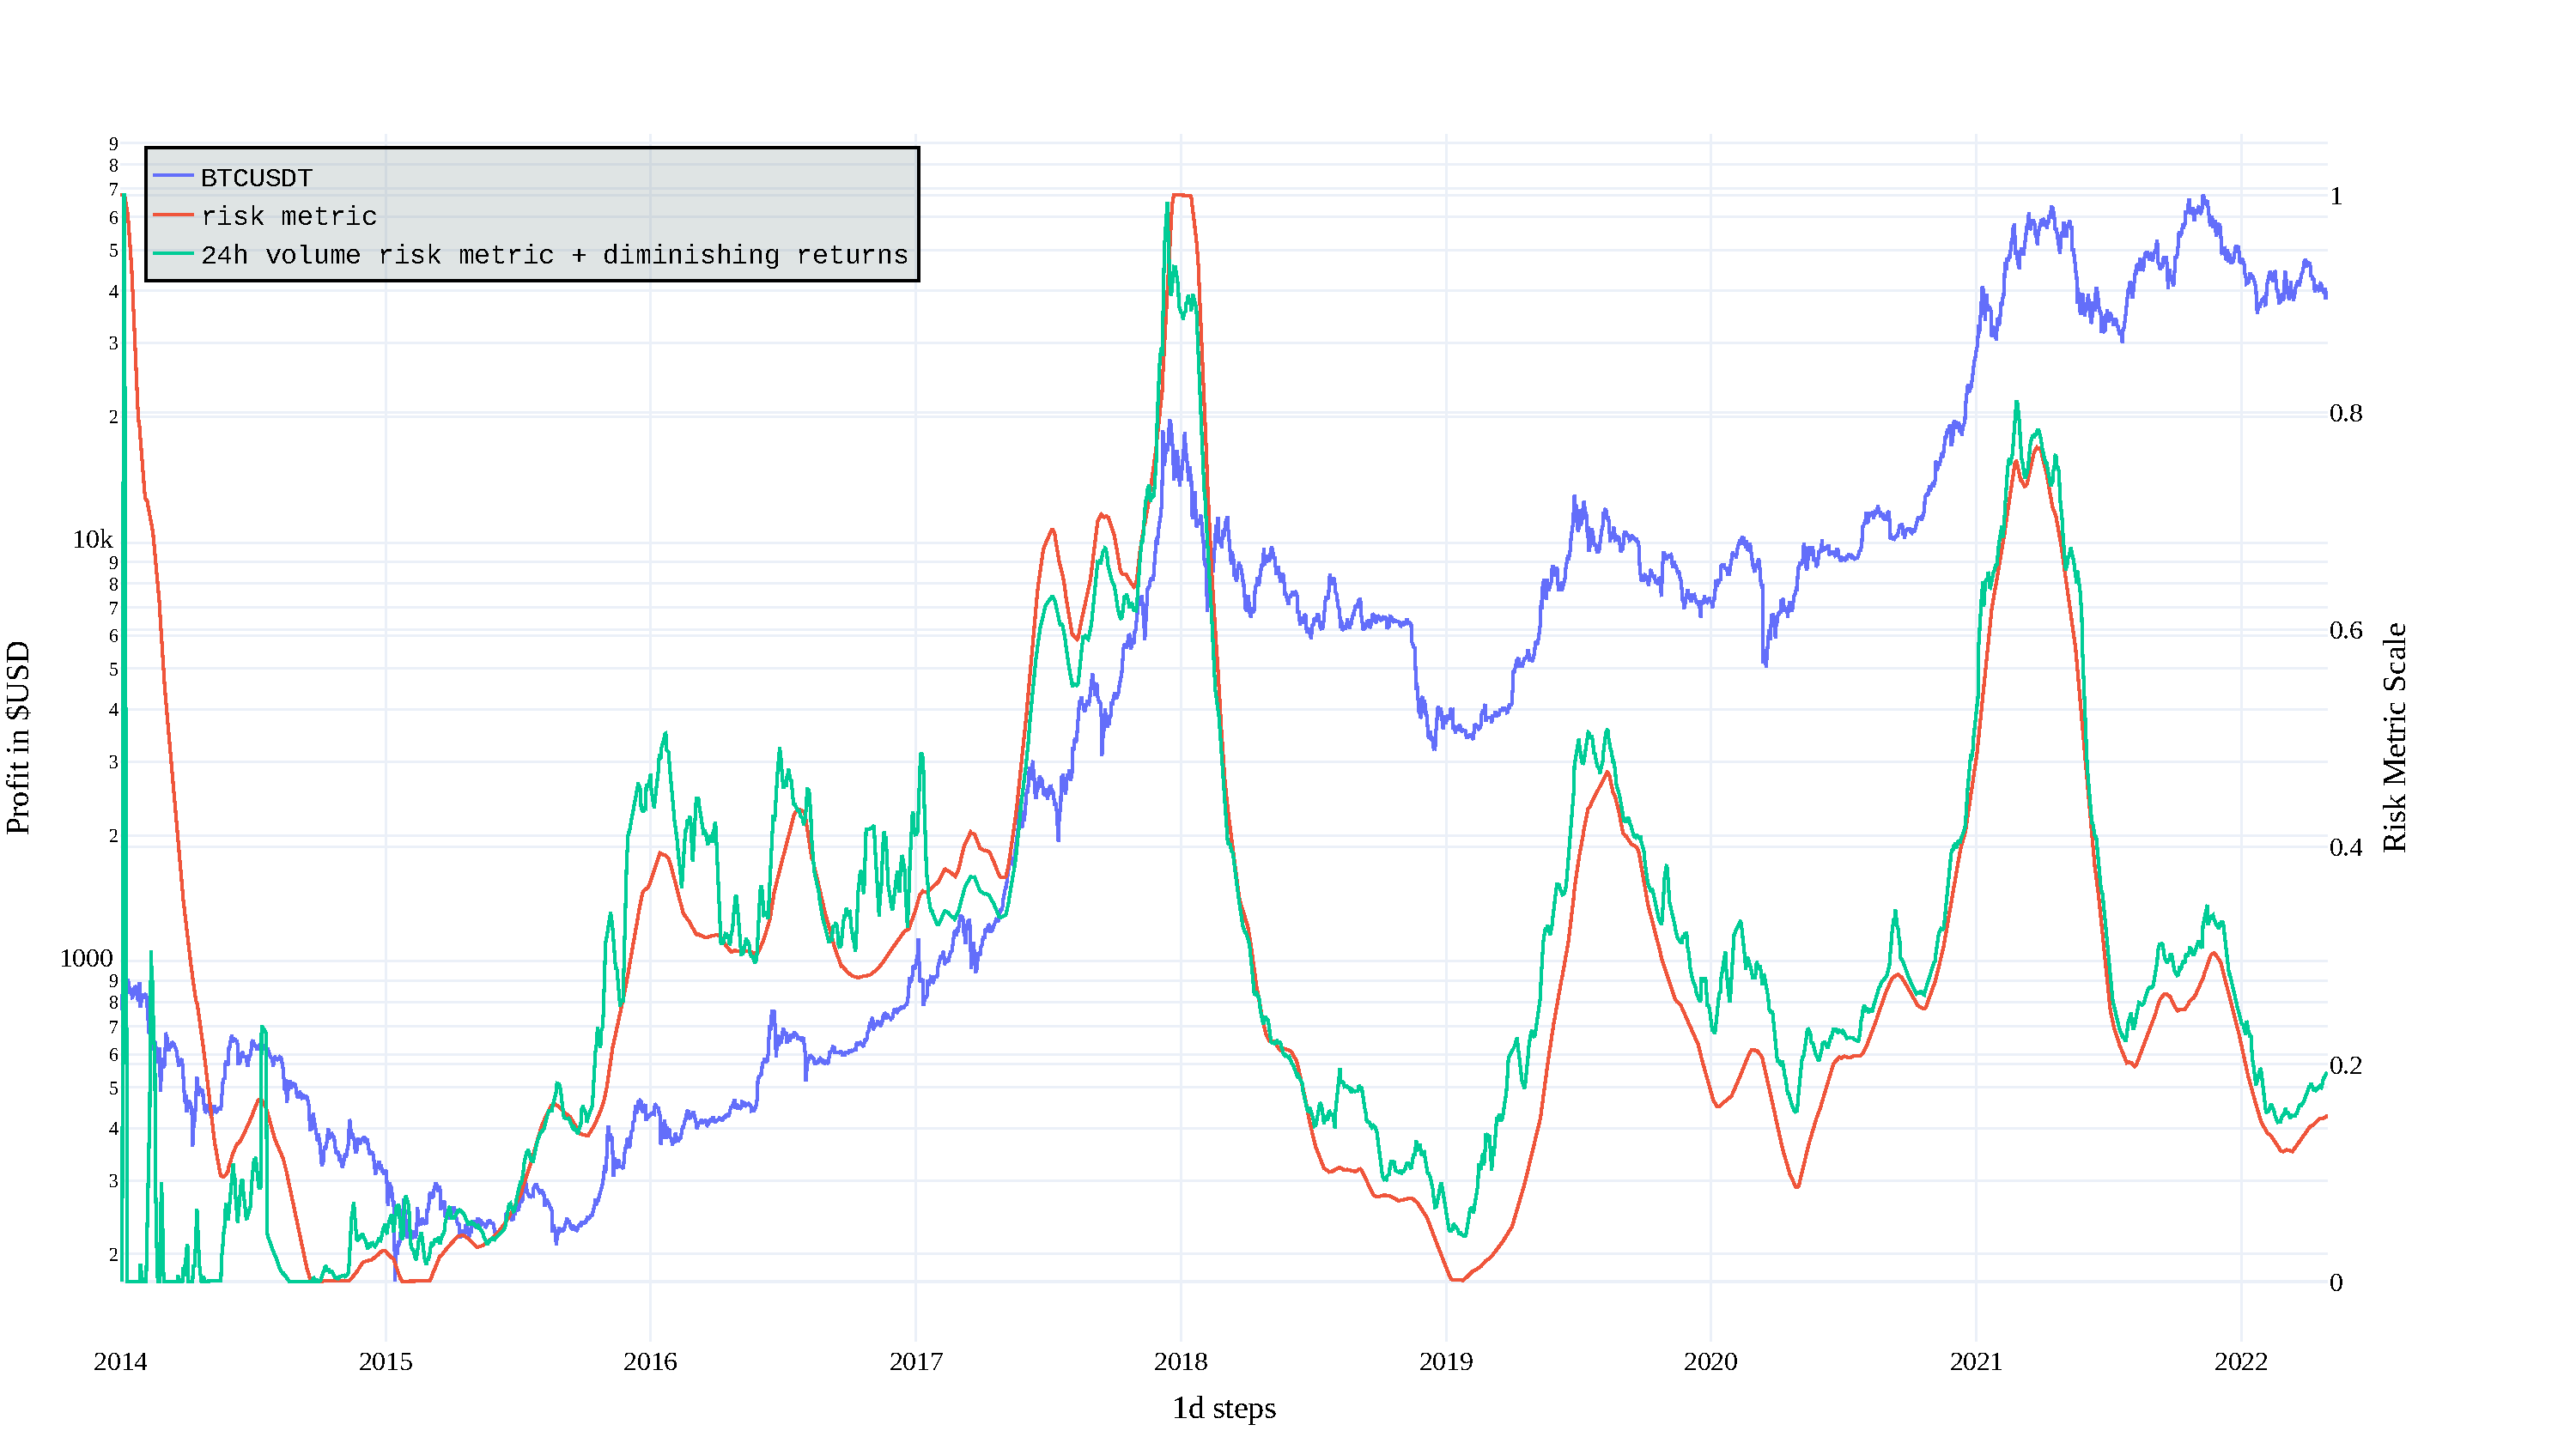
\includegraphics[width=\columnwidth]{figures/24volume-riskmetric-dimreturns.pdf}
    \caption{Log-log graph comparing the Bitcoin price and its \$USD volume.}
    \label{figure-24volume-riskmetric-dimreturns}
\end{figure}


\subsection*{Machine Learning Optimization}
\label{subsection-ml-optimization}

In this section the last optimization is touched upon. Machine Learning is a very vast subject. For the thesis's purpose, the time series prediction is our subject. Predictions of these types require a good model to learn upon to work well, otherwise the results are questionable at best. In this section the time series prediction is used to predtict the price of Bitcoin. This result could be later correlated with the previous achieved findings.

The \texttt{AutoTS} Python library~\cite{autots} is used to make the predictions. One of the ways that the machine learning optimization could be incorporated to the other tactics is the following. Every day it would predict the price for the following X (e.g. 10) days. Depending on how well the prediction is, it would either make the risk bigger or smaller.

The forecasts got are too linear and usually too optimistic to be of any bigger use. Some forecast can be seen in Figure \ref{figure-autots-prediction}
Since the results got are not reliable, the machine learning optimization is not evaluated. Further investigation of the machine learning algorithm would be needed.

\begin{figure}[!hbt]
    \centering
    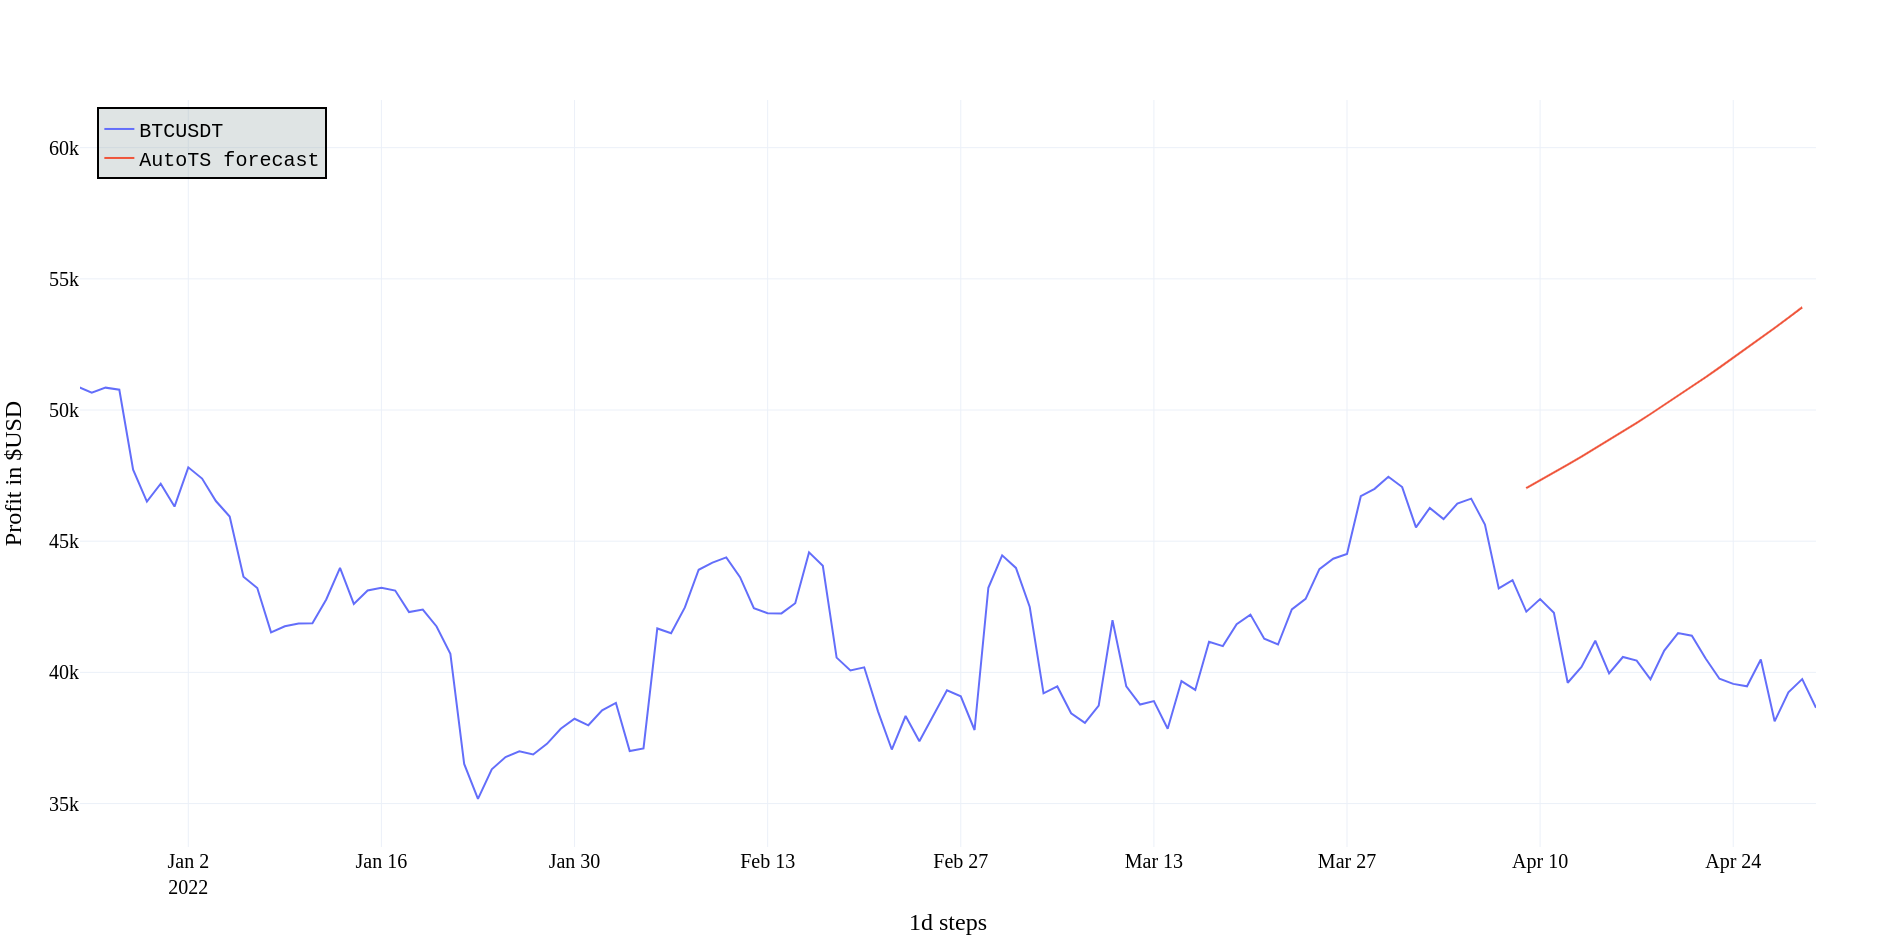
\includegraphics[width=\columnwidth]{figures/autots-prediction.png}
    \caption{AutoTS~\cite{autots} prediction.}
    \label{figure-autots-prediction}
\end{figure}

\section{Evaluating Strategies}
Let us put the implemented strategies to use. In this section the correct evaluation strategy is found and discussed strategies of Section \ref{section-strategies} evaluated.

Some of the strategies, like machine learning optimization \ref{subsection-ml-optimization}, is not evaluated since its usefulness has not been proved in the previous section.

\subsection*{Finding the Optimal Evaluation Strategy}
By rigorous testing I have found that the ideal evaluation strategy is as follows: ...


\subsection*{Testing portfolio C}
Let us start with the original bitcoin risk metric proposed in Section \ref{subsection-50week50days}. We will first test the metric on Bitcoin only (portfolio C).

\begin{figure}[!hbt]
    \centering
    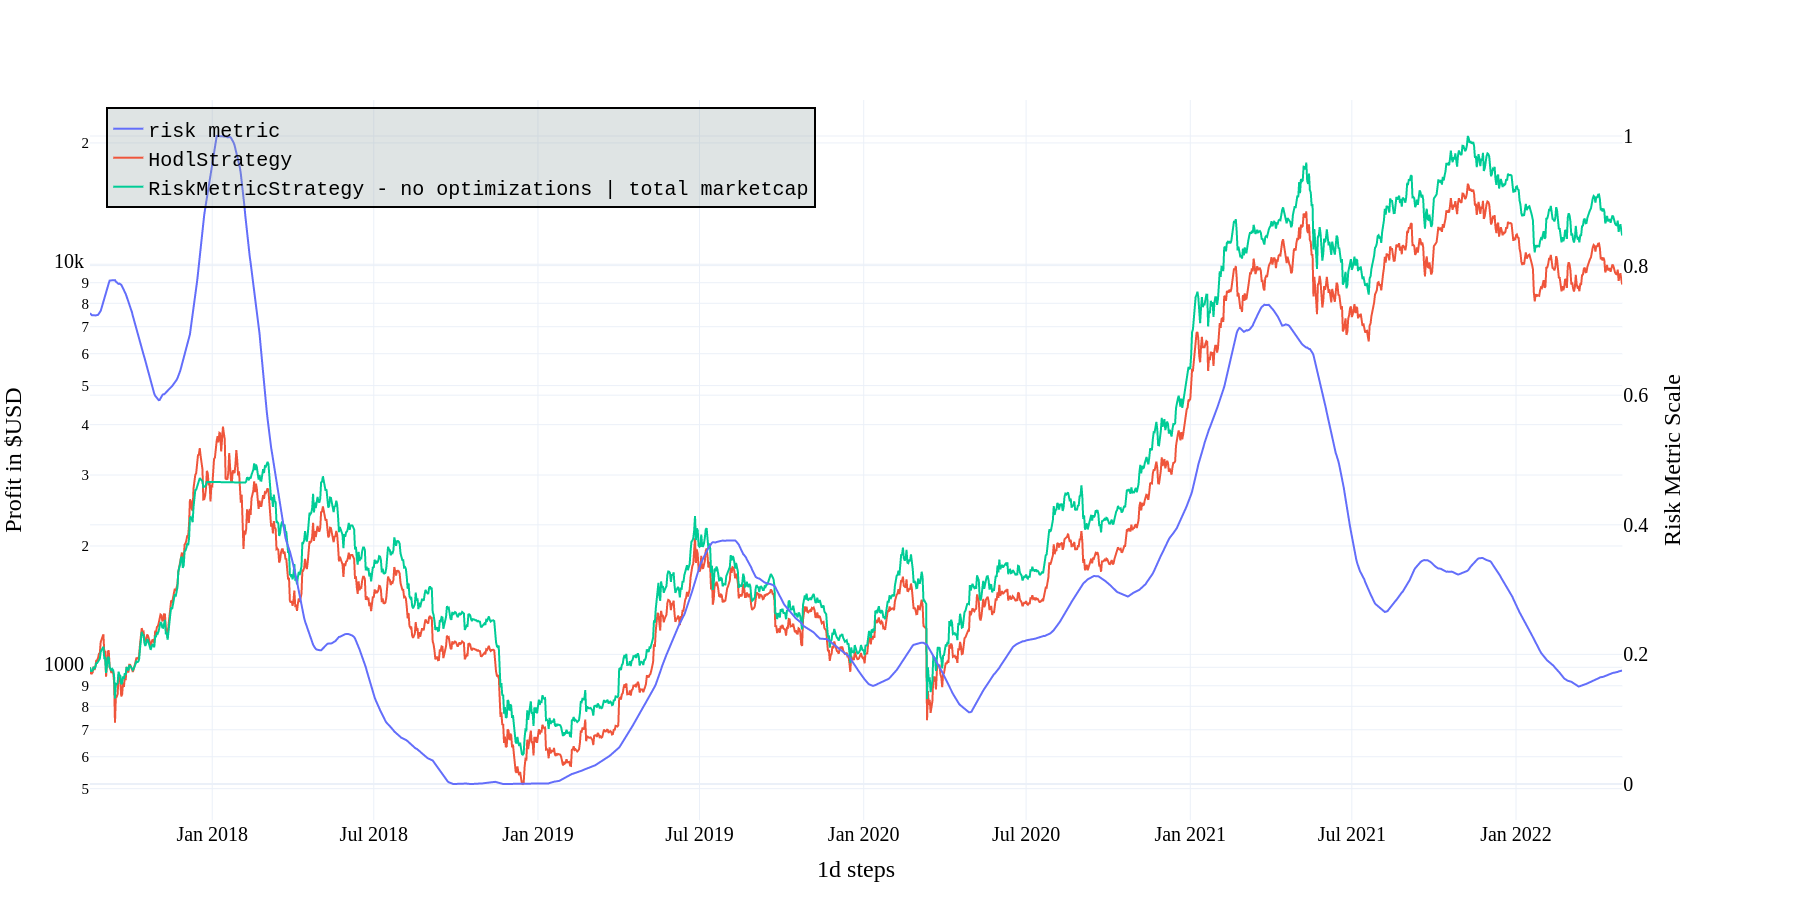
\includegraphics[width=\columnwidth]{figures/strat-eval1.png}
    \caption{Strategy evaluation.}
    \label{figure-strat-eval}
\end{figure}

\begin{figure}[!hbt]
    \centering
    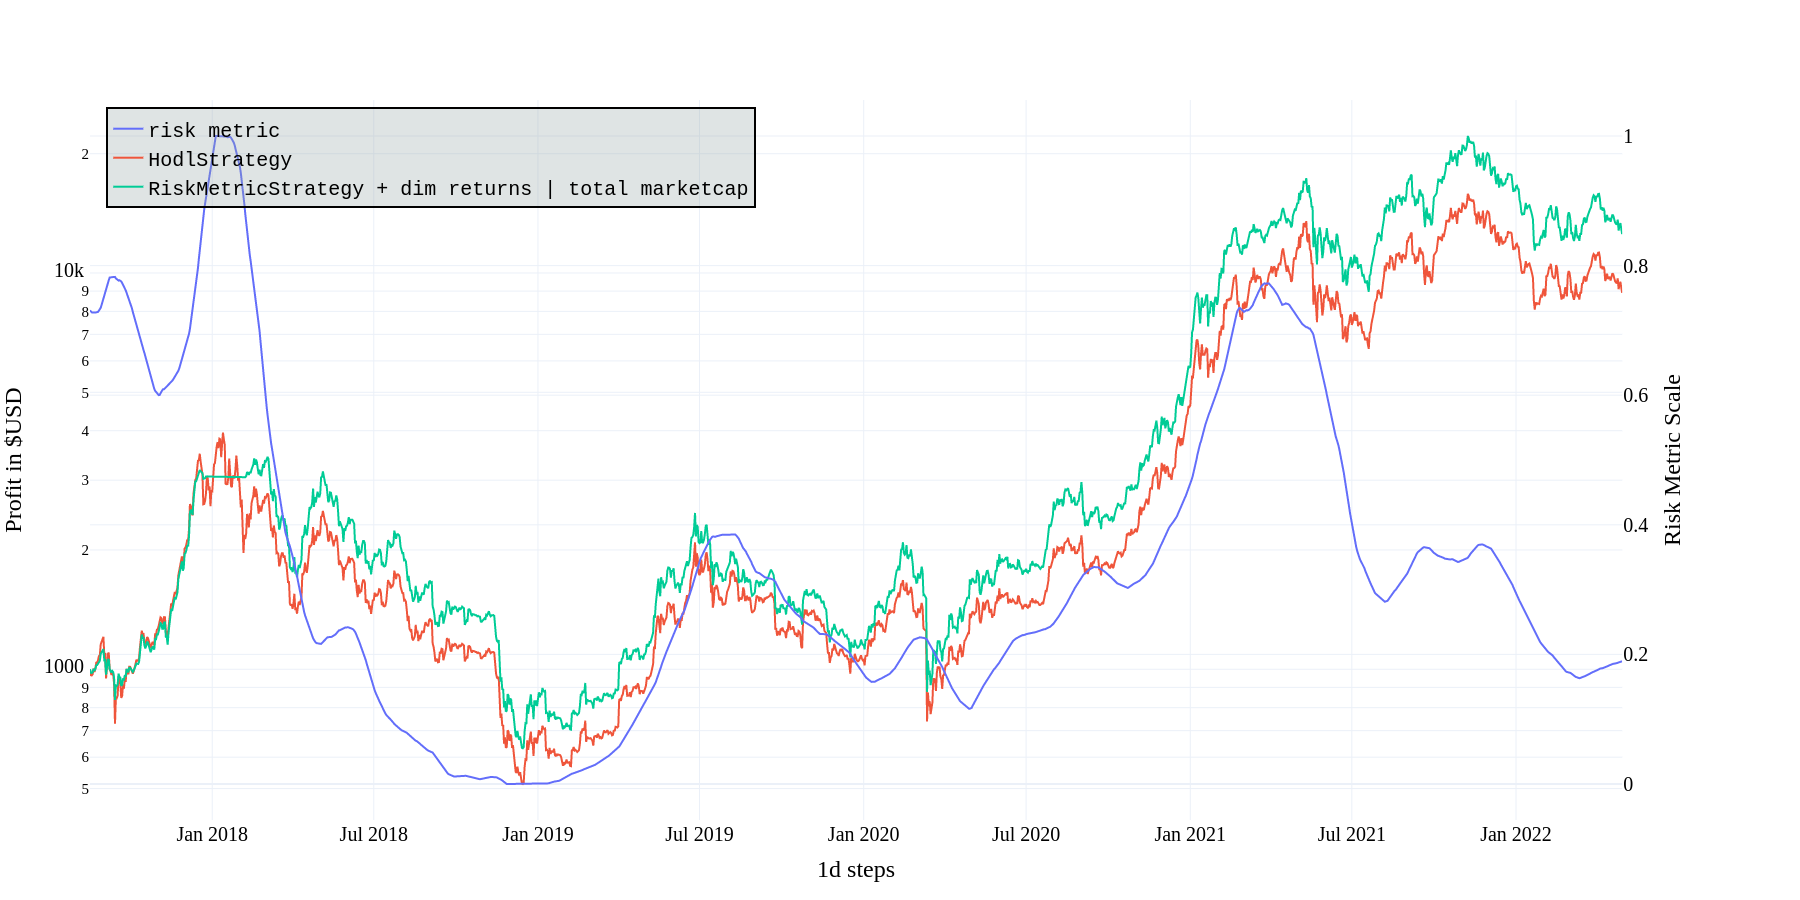
\includegraphics[width=\columnwidth]{figures/strat-eval2.png}
    \caption{Strategy evaluation.}
    \label{figure-strat-eval}
\end{figure}

\begin{figure}[!hbt]
    \centering
    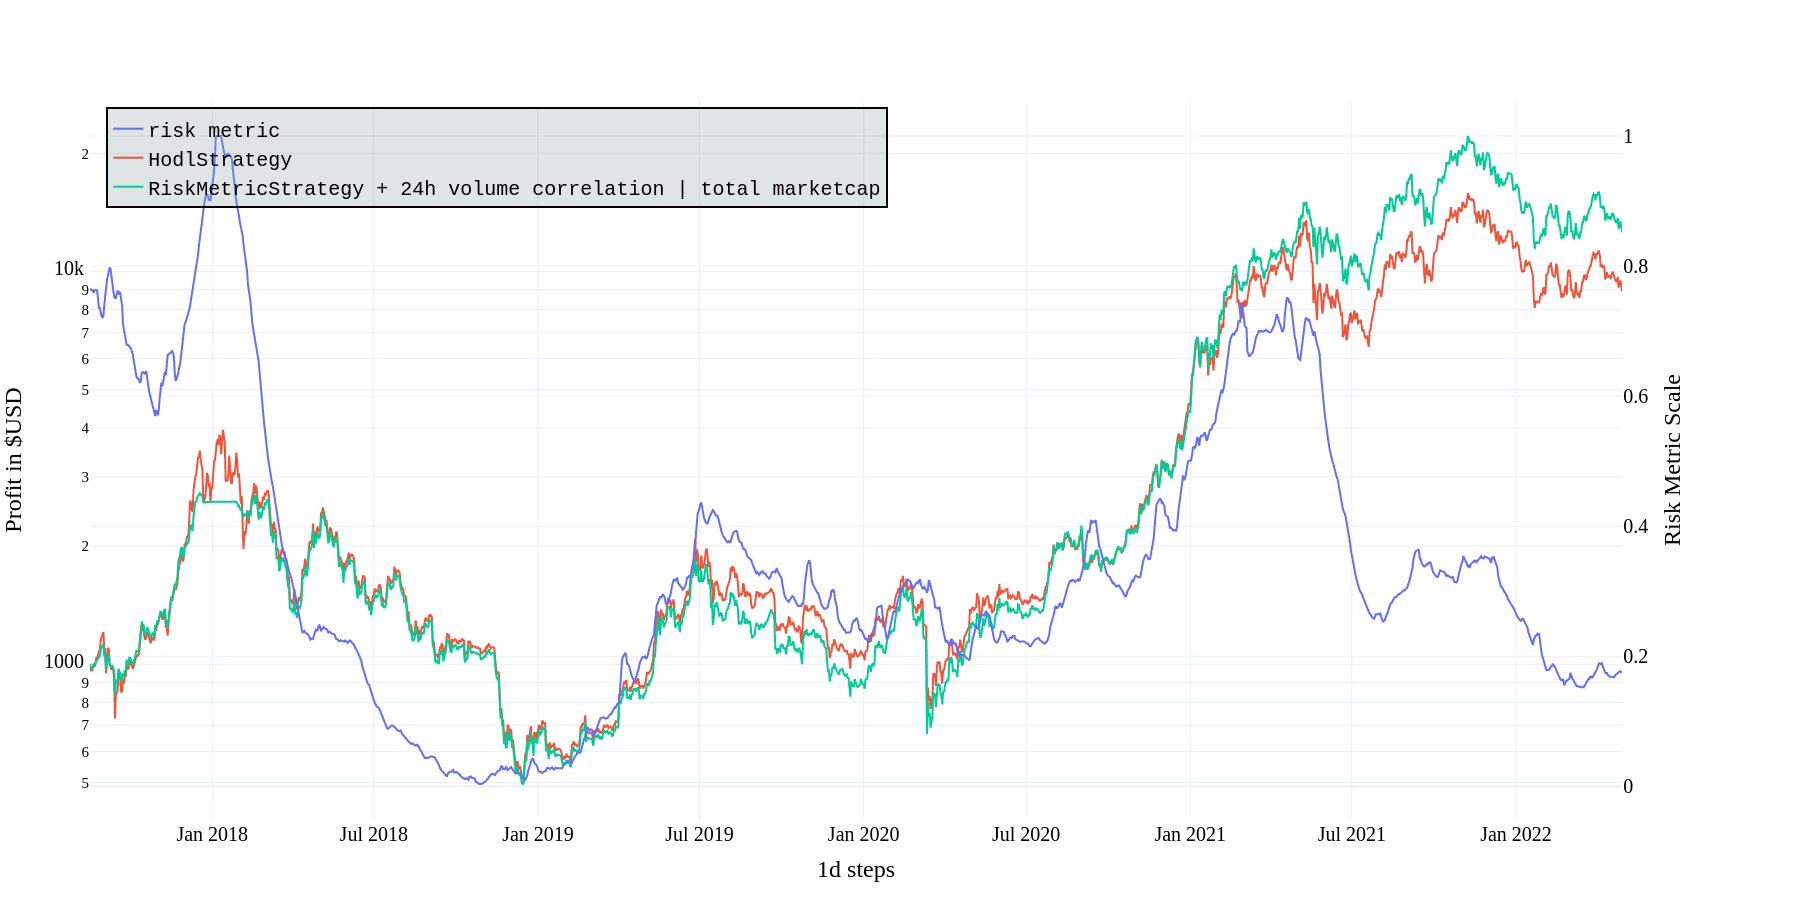
\includegraphics[width=\columnwidth]{figures/strat-eval3.png}
    \caption{Strategy evaluation.}
    \label{figure-strat-eval}
\end{figure}

\subsection*{Evaluating Bitcoin Risk Metric}

\subsection*{Evaluating Total Market Cap Risk Metric}

\subsection*{Evaluating Bitcoin Risk Metric Correlated With Daily Volume}

\section{Testing For Day Trading}
Optimizing for long term investing is great, it has a lower risk than trading throughout the day while still keeping good profits. But one thing it cannot do is to gain capital fast, that is where day trading can shine. In this section the adaptive strategies are tested on a few several days window with 5 minute OHLCV portfolio data.

\subsection*{Creating the Strategy}
Instead of looking for loing moving averages of 50 weeks and days as before, we will look at a different indicator. Moving average of 6 hours---that means 72 ticks of 5 minute data---is used as the metric. The moving average smooths out the rigidity of the 5 minute data and allows us to exploit the rising and falling trends during the day. It is a form of range trading \ref{section-range-trading} where we take advantage of the fact that cryptocurrencies fluctuate multiple times during a day.

\subsection*{Strategy Evaluation}
The strategy is tested on bitcoin only. It does not make much sense to test the strategies with many cryptocurrencies, because the strategy is tailored to one asset only. Theoretically, a portfolio with many cryptocurrencies can run this strategy individually per every currency.

The basic evaluation strategy is to sell at the local maxima of the moving average and buy at the local minima. Thus trying to buy low and sell high. The local maxima and minima take the 5 points from each side into consideration---this prevents too many extrema next to each other, which would not be useful.

Three date range have been chosen to evaluate the results. A date range with a falling, rising and changing trend. The results can be seen in Figures \ref{figure-short-term-rising}, \ref{figure-short-term-falling} and \ref{figure-short-term-changing}.

\begin{figure}[!hbt]
    \centering
    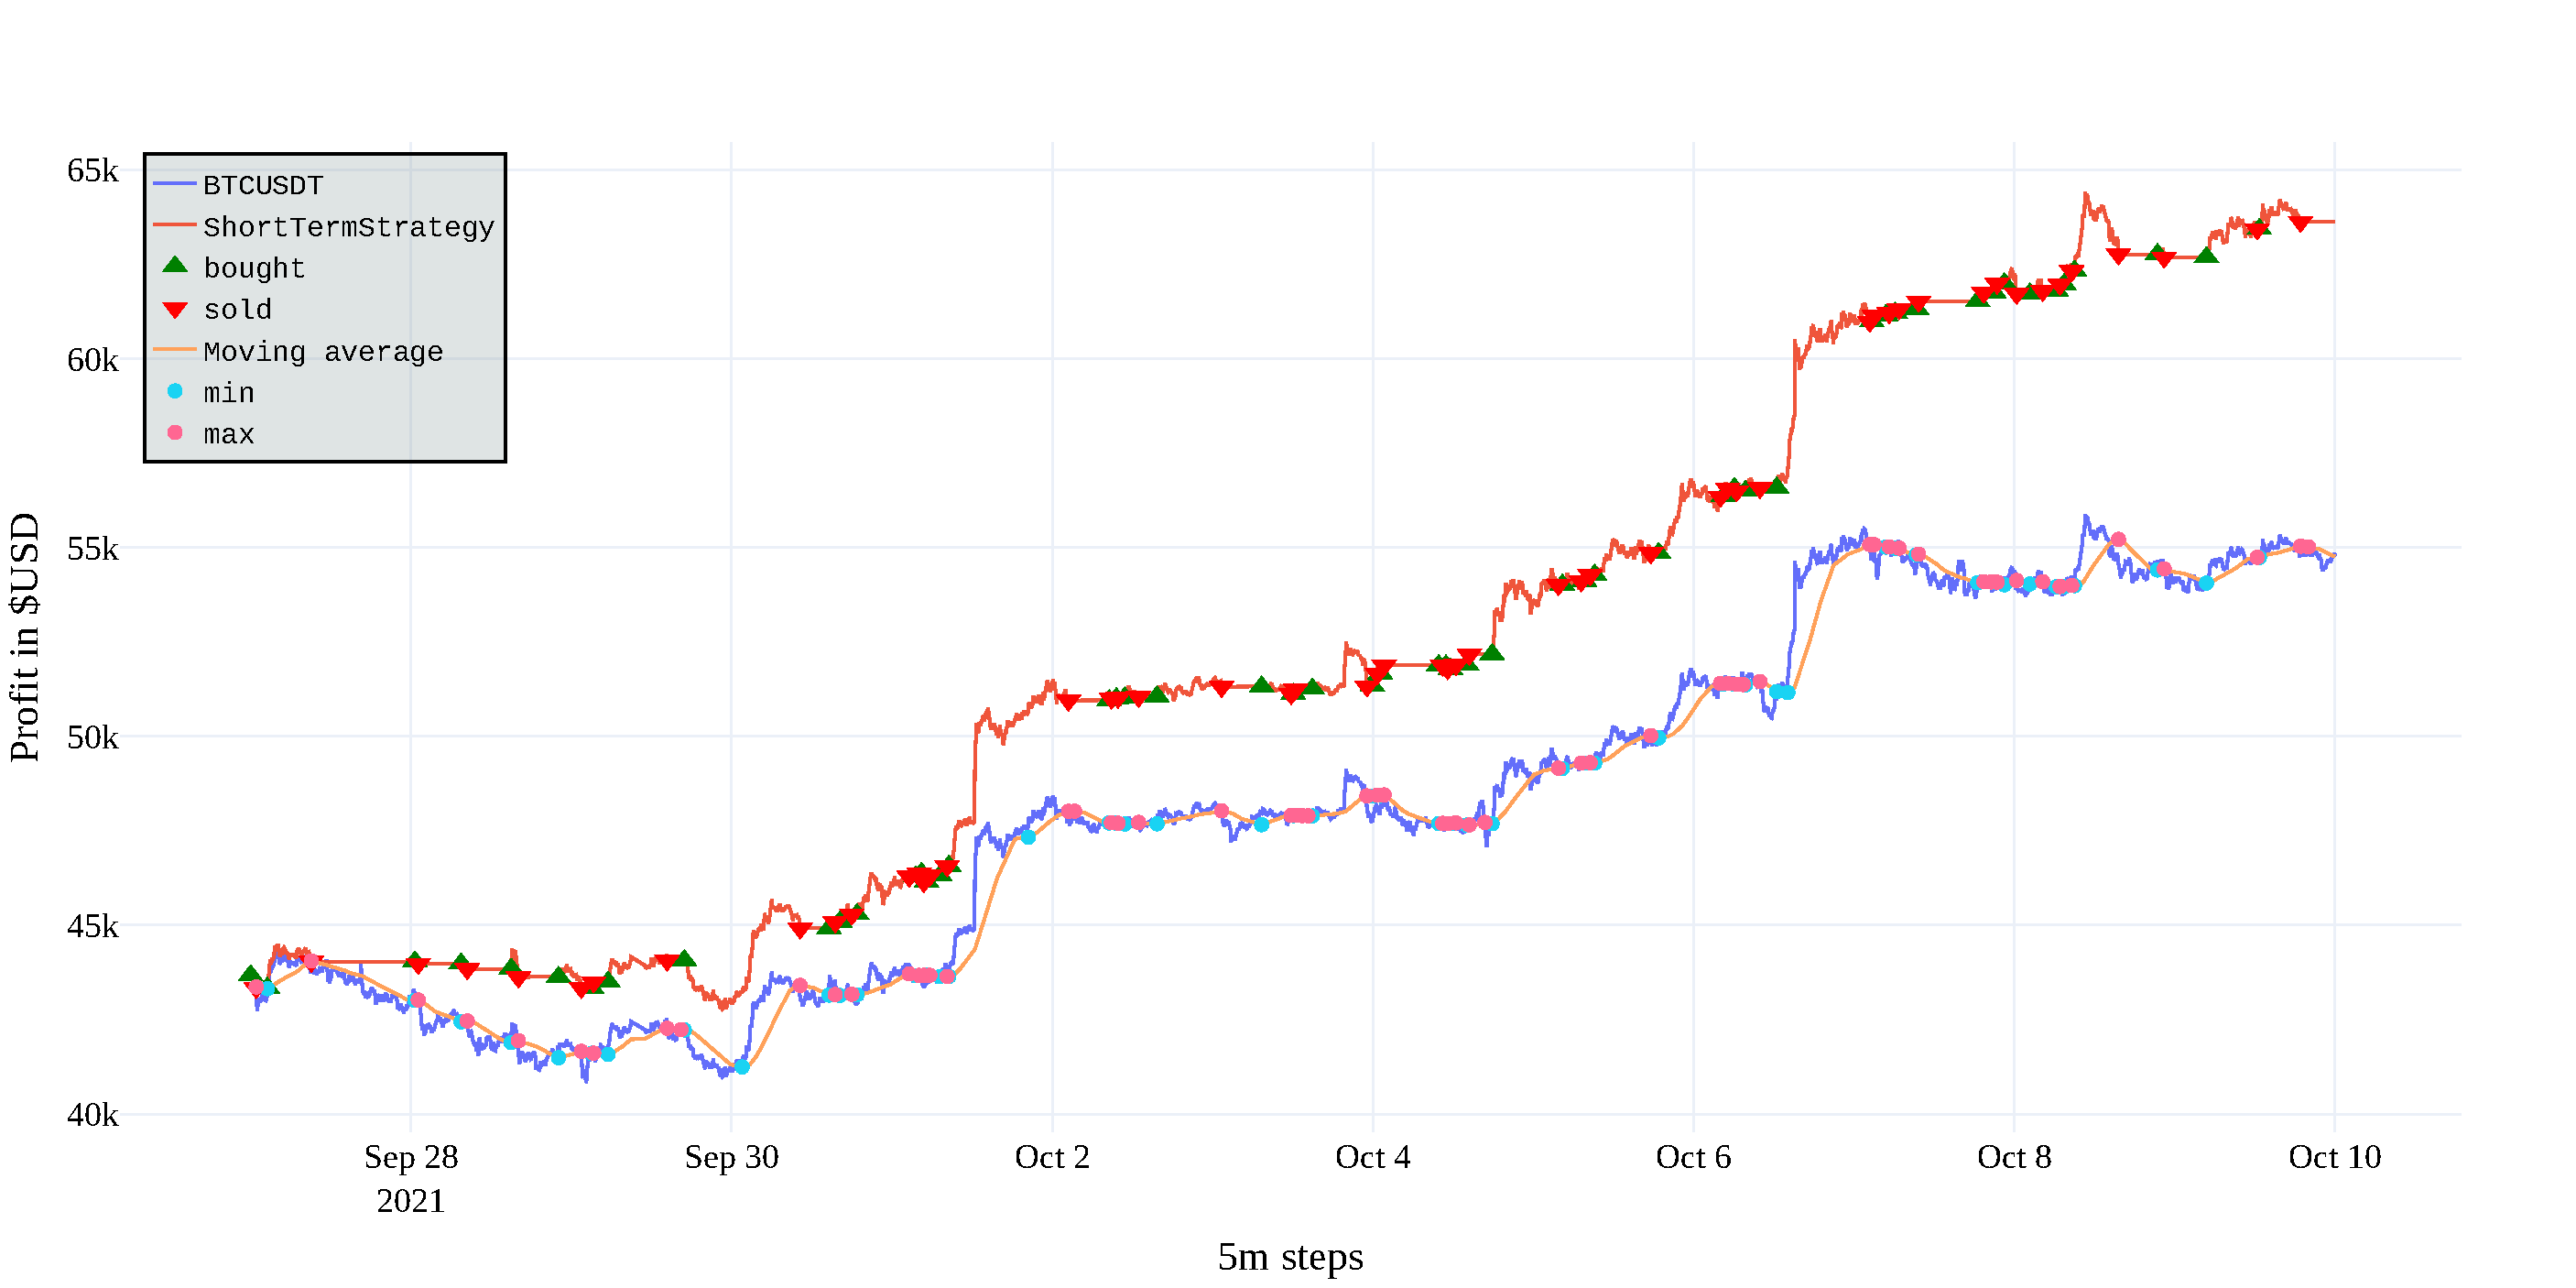
\includegraphics[width=\columnwidth]{figures/short-term-rising.pdf}
    \caption{27th Sep--10th Oct 2021 rising trend that registered rise from \$43000 to \$55000.}
    \label{figure-short-term-rising}
\end{figure}

\begin{figure}[!hbt]
    \centering
    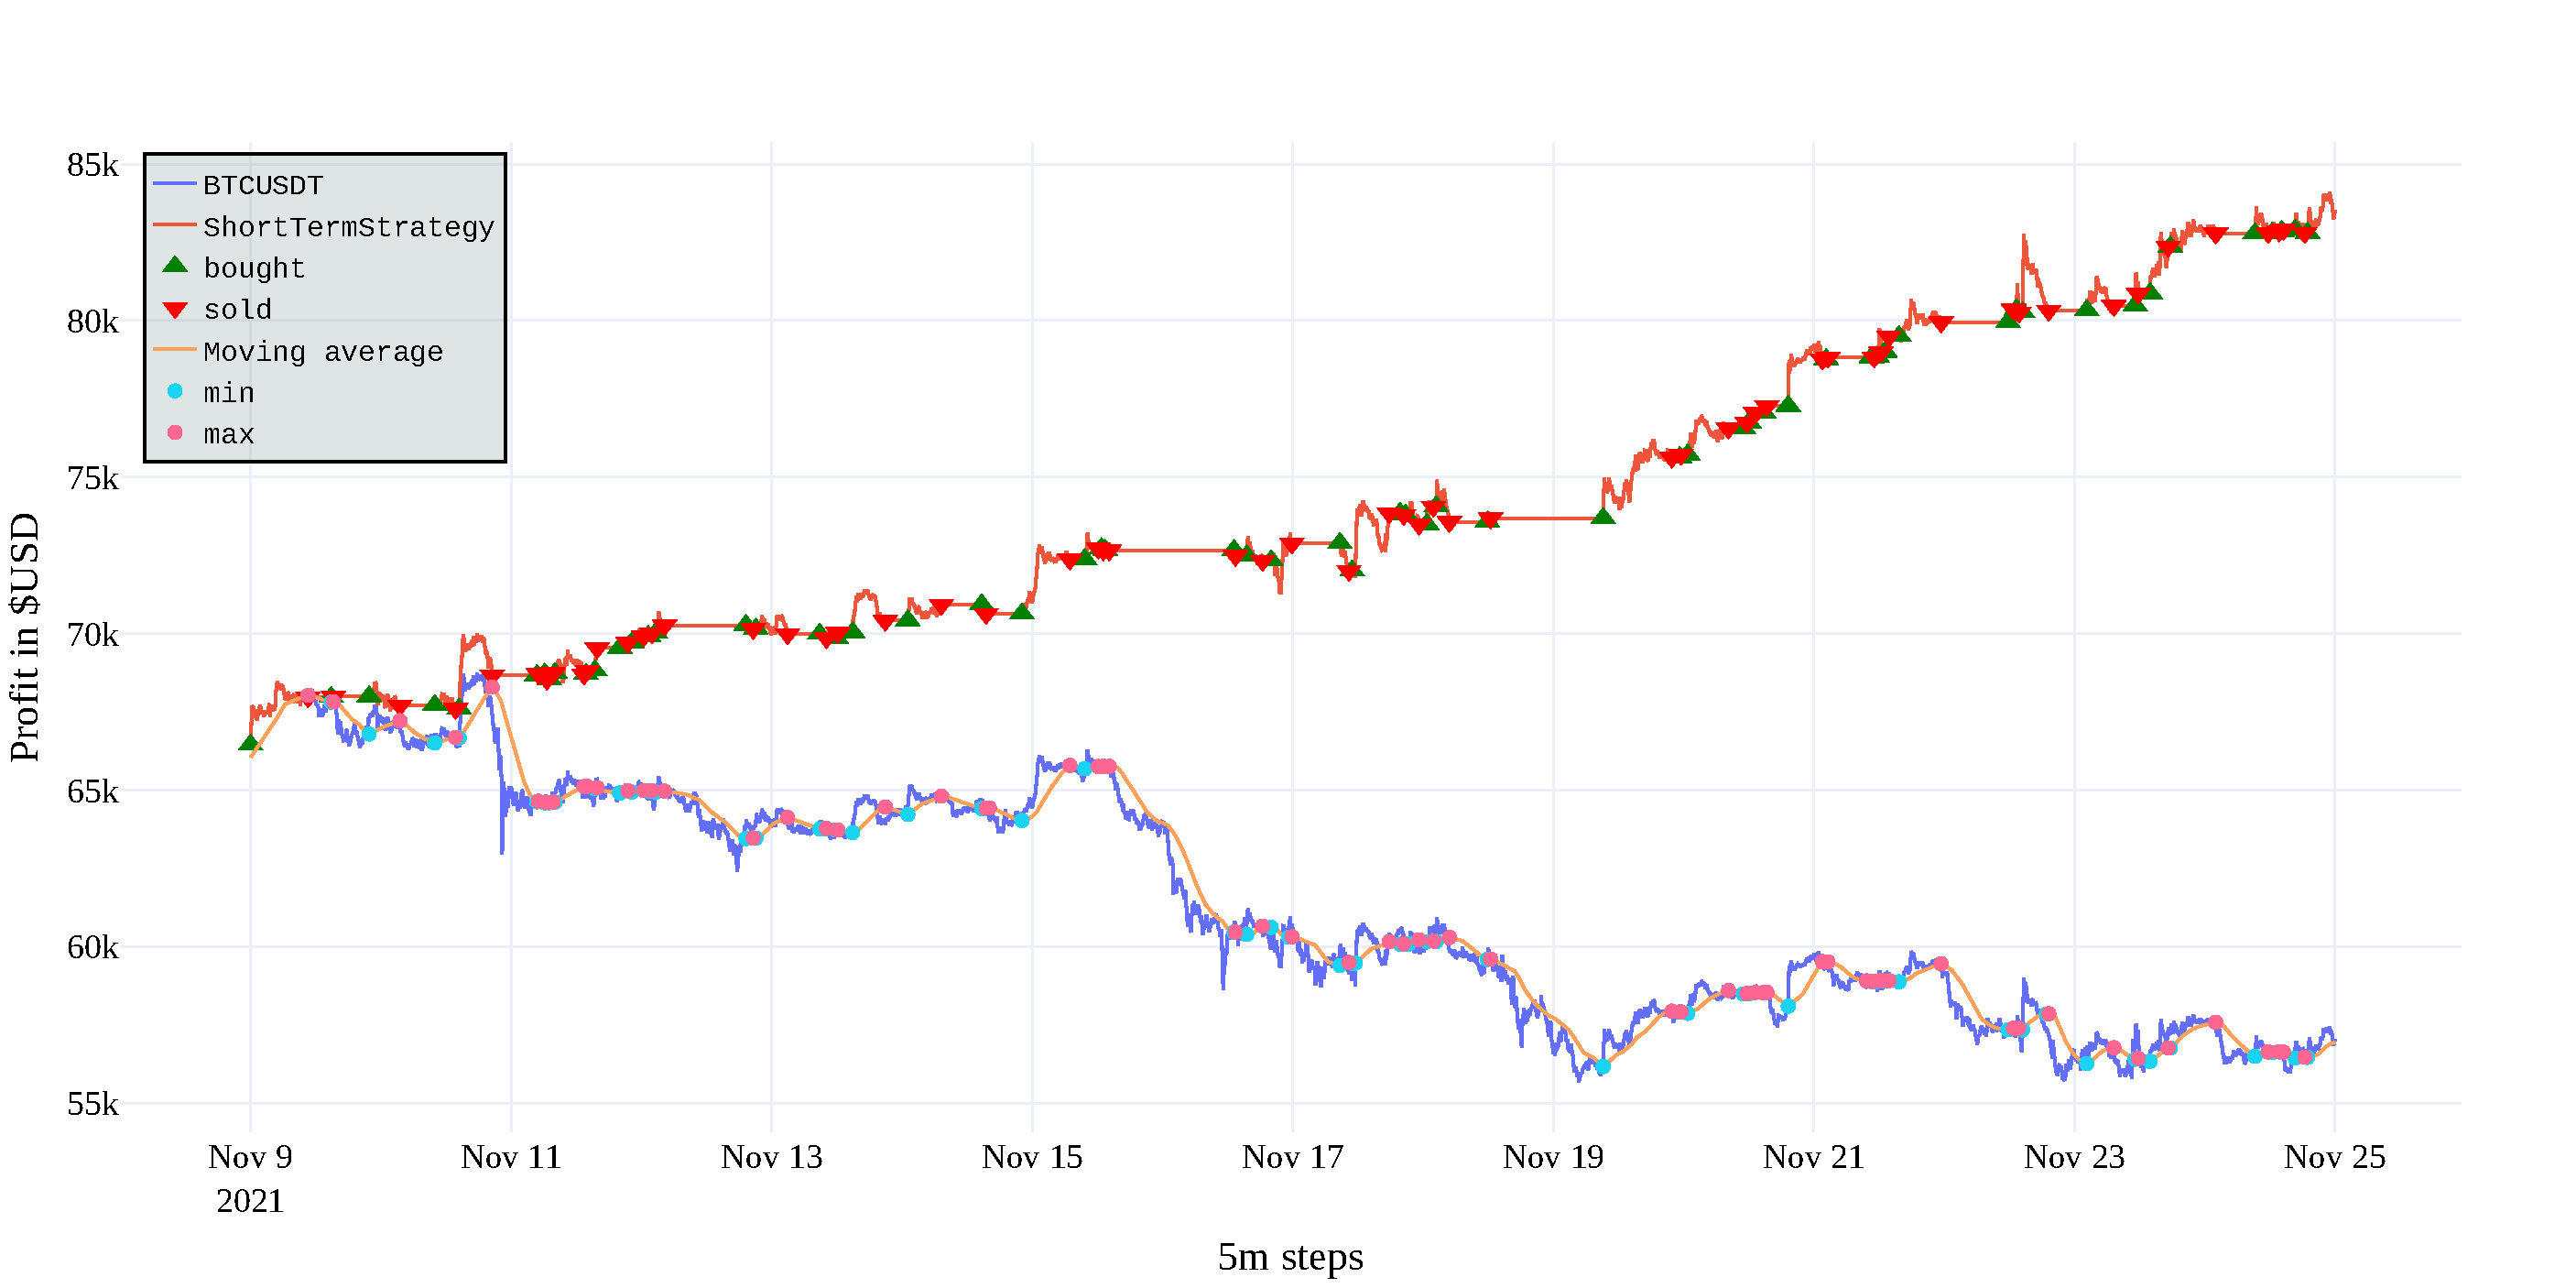
\includegraphics[width=\columnwidth]{figures/short-term-falling.pdf}
    \caption{9th Nov--25th Nov 2021 falling trend that registered fall from \$65000 to \$55000.}
    \label{figure-short-term-falling}
\end{figure}

\begin{figure}[!hbt]
    \centering
    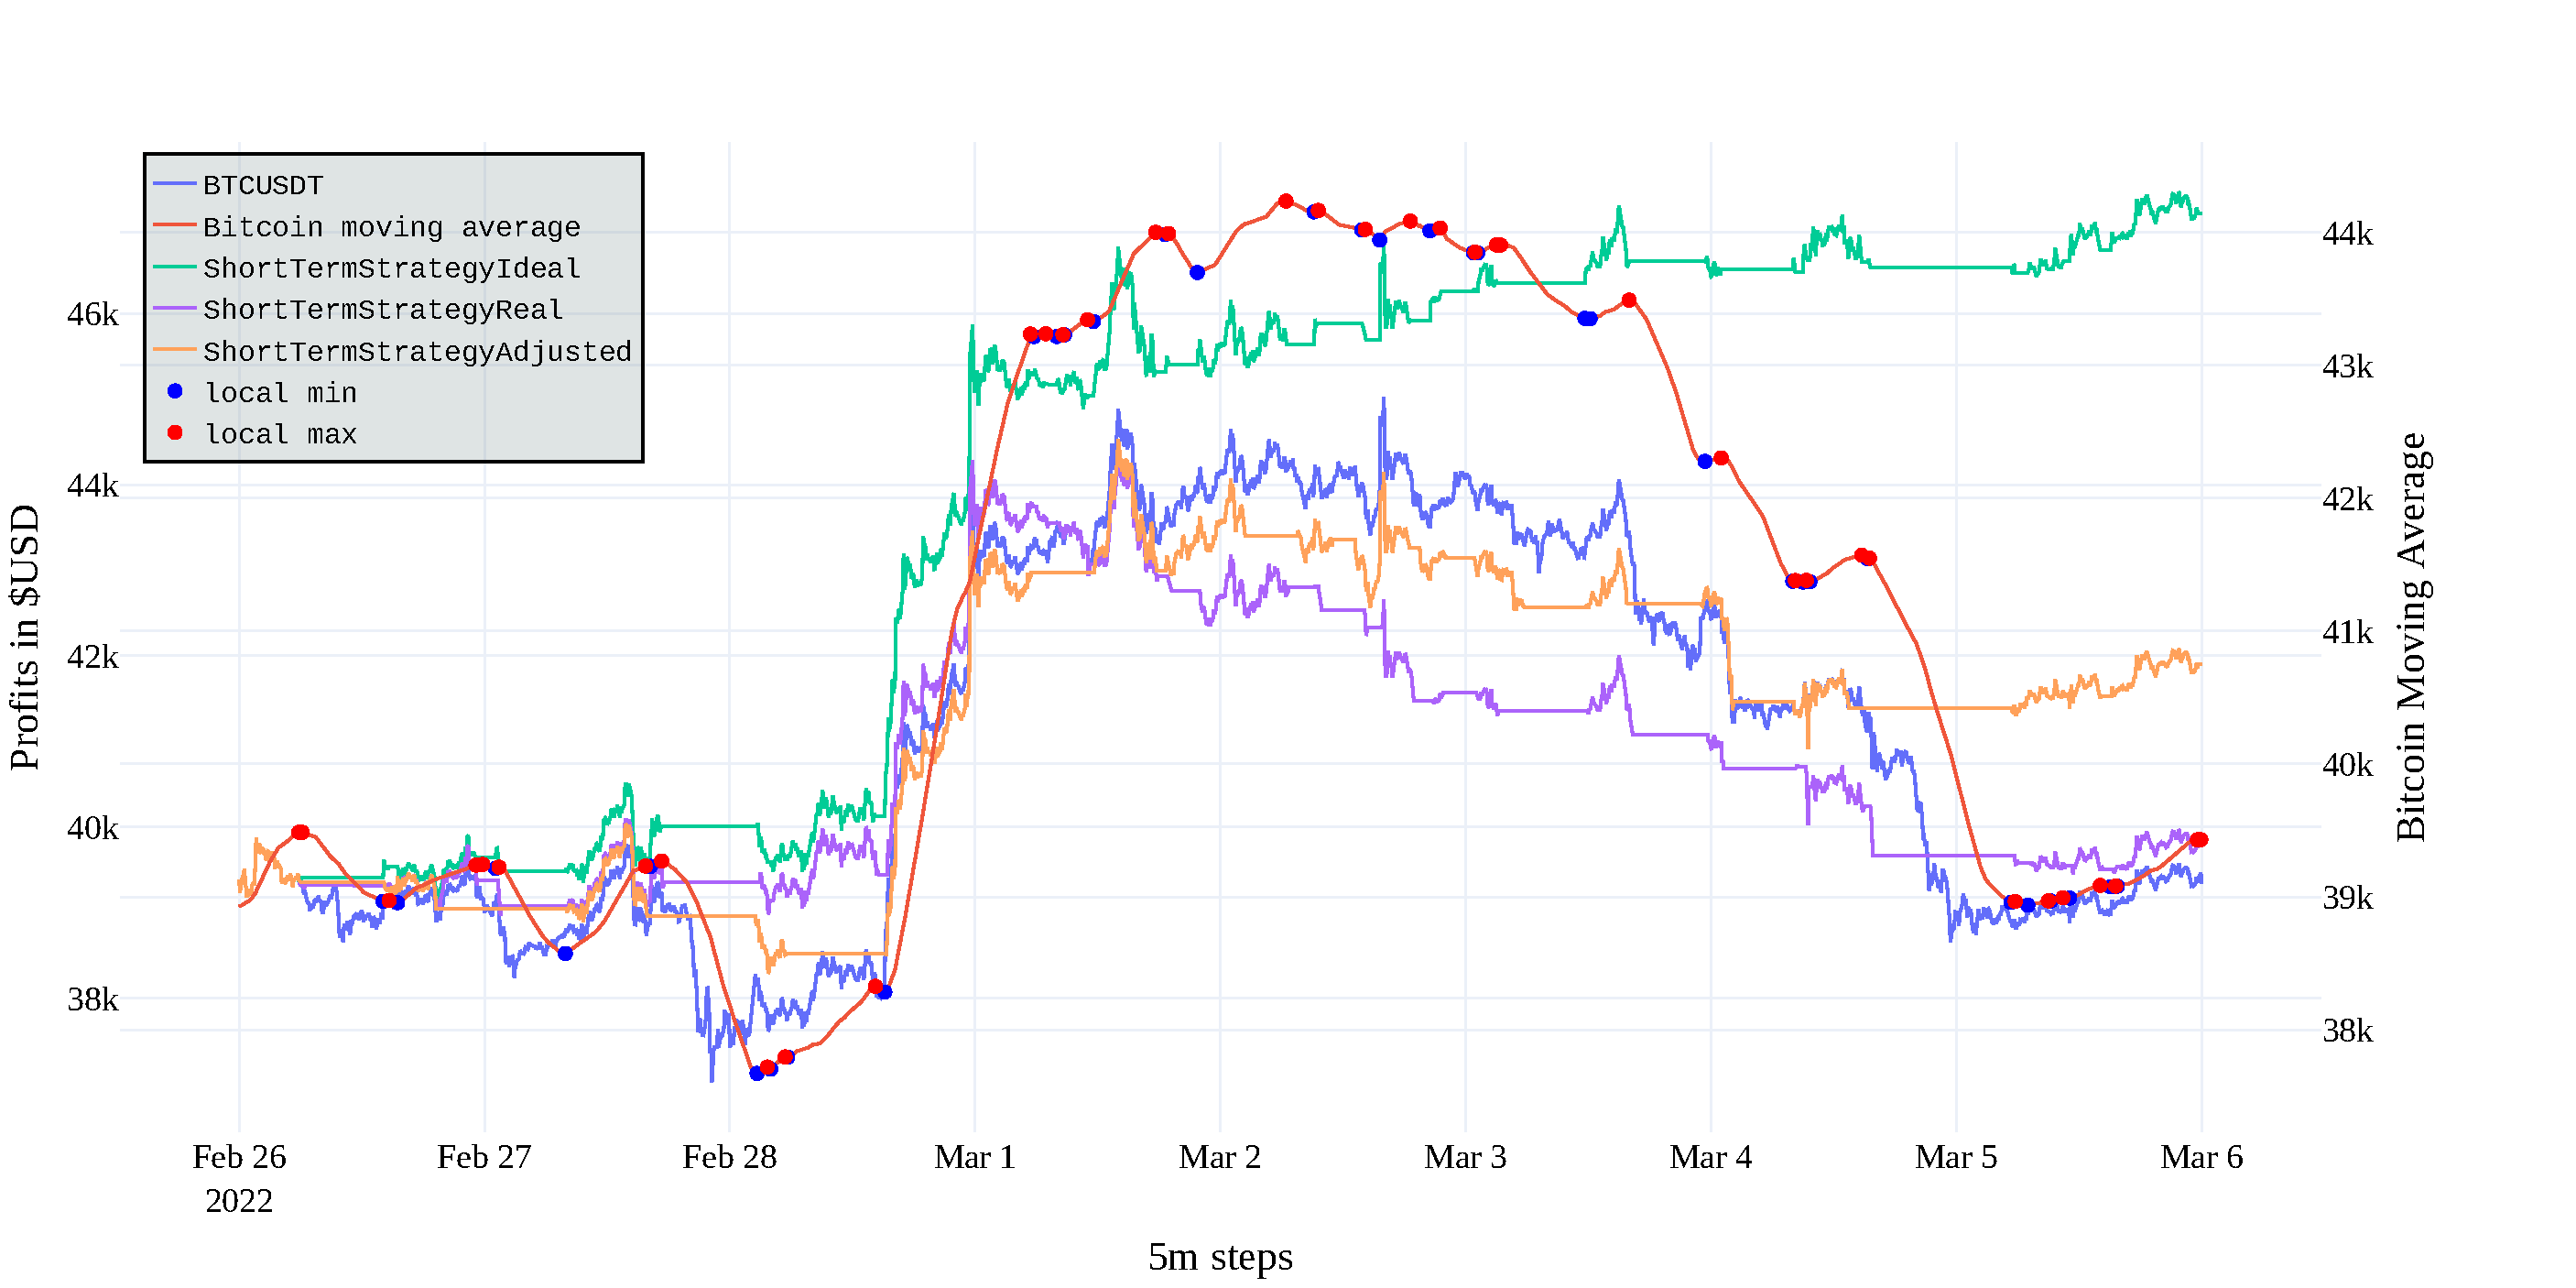
\includegraphics[width=\columnwidth]{figures/short-term-changing.pdf}
    \caption{6th Feb--26th Mar 2022 changing trend.}
    \label{figure-short-term-changing}
\end{figure}

Surprsingly, all the date ranges experienced somewhat constant profits, with the falling date range's difference against HODL being most noticable. Here it must be said that no exchange fees are taken into the account. Most of the individual trades generate a little profit that only accumulates over time---meaning that exchange fees would diminish the results noticable and must be taken into the account when considering using the strategy. Nevertheless, the results are pleasing.

Let us see how the strategy fares when applied over several months. The date range chosen is February until April of the year 2022. The results can be seen in \ref{figure-short-term-long}. The profits trend upwards in an almost linear fashion. The strategy has shown very promising results so far.

\begin{figure}[!hbt]
    \centering
    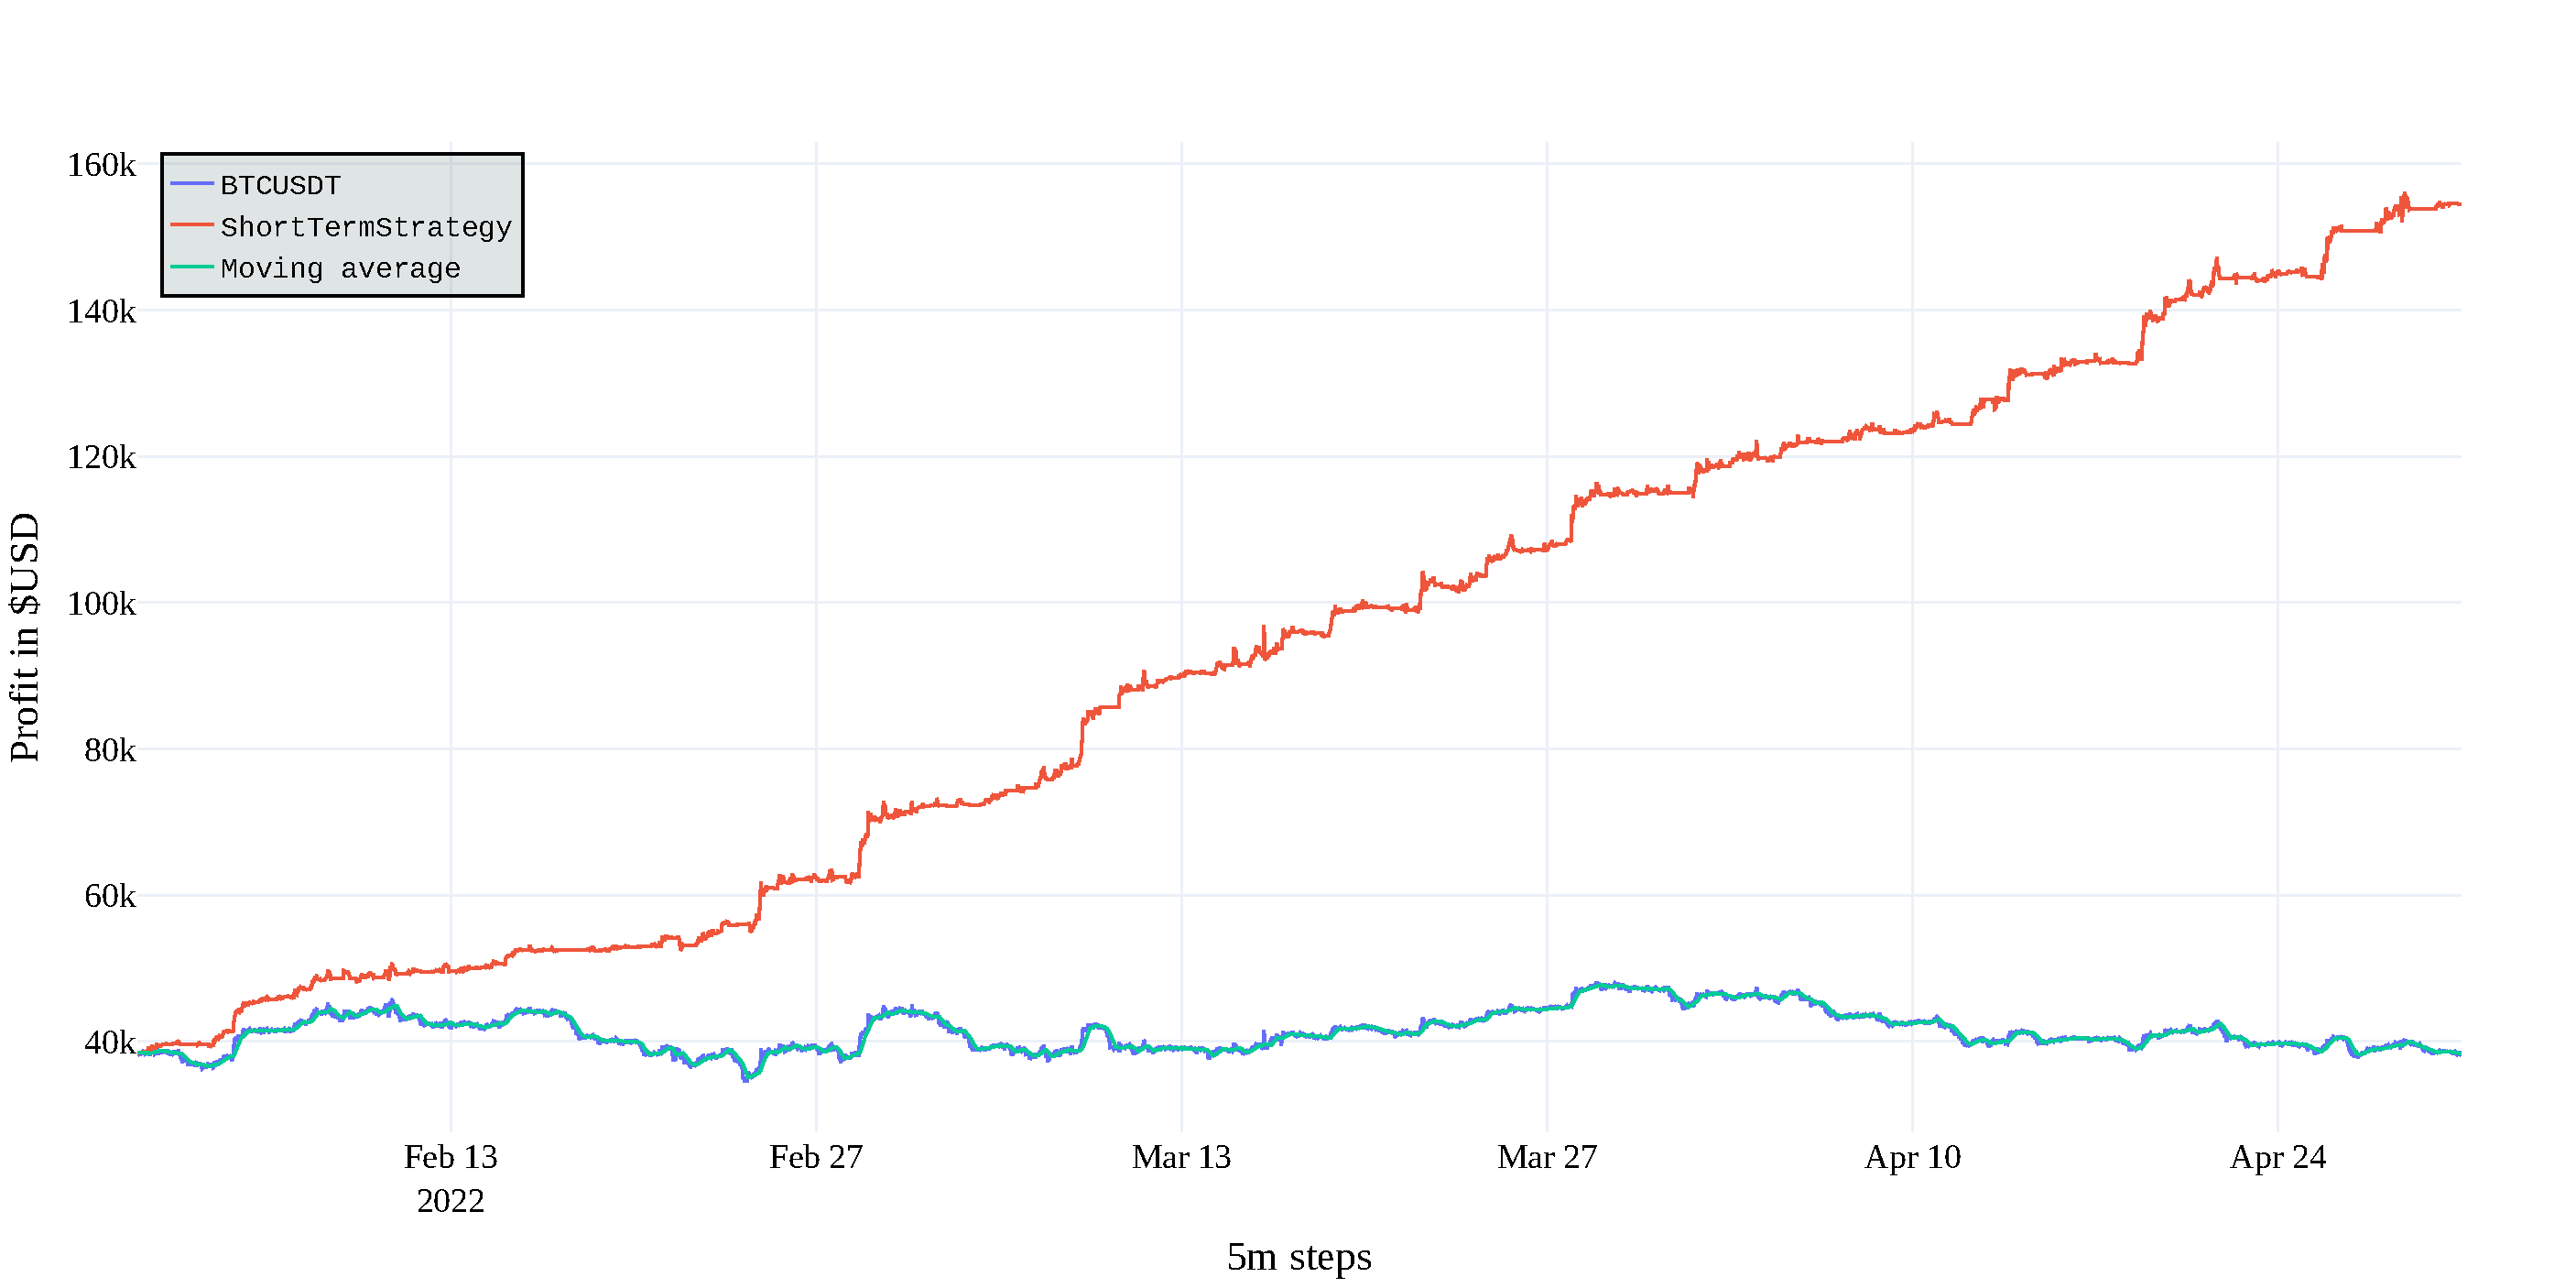
\includegraphics[width=\columnwidth]{figures/short-term-long.pdf}
    \caption{6th Feb--26th Mar 2022 changing trend.}
    \label{figure-short-term-long}
\end{figure}

\chapter{Limitations and Further Improvements of Practical Deployment}
\label{chapter-limitations-and-improvements}

So far we have only discussed the backtesting framework developed. For practical use, actual API calls to cryptomarket exchanges such as Binance\footnote{\url{https://www.binance.com/}} or Coinbase\footnote{\url{https://www.coinbase.com/}} would be needed.

This would require either heavily changing the existing framework or creating a new project entirely. I would design in such a way, that the working backtesting framework would be solely for experimenting with new strategies or validating the chosen strategies for the current day. The projects could work in conjecture this way. The practical deployment would send the new daily data to the backtesting framework which would then send a signal to the deployment on what to do---buy, sell, rebalance, etc.

This would also require working with always up-to-date data, not just historical. Some different API endpoints may be used.

Other improvement to the overall framework would be to add the exchange fees when the investor buys or sells. The current results would get a bit diminished by this fact. This abstraction for the thesis has been approved by the supervisor.

\section{TODO: Comparison to Existing Solutions}
\begin{enumerate}
    \item 3Commas
    \item Cowen Risk Metric
\end{enumerate}

\section{Further Ideas and Involvement}
The science and technical analysis of cryptocurrencies is a vast subject and time is limited. There is an infinite number of things to test and analyze. The framework itself could be improved. Below are some strategies, optimizations and ideas that I considered during the thesis and that can be worked on in further involvement.

\subsection*{Strategies}
Top 7 trading cryptocurrencies CoinGecko API endpoint could be used to buy trending cryptocurrencies based on the believe that they would rise soon.

It would advisable to add trending strategies to portfolio dynamically during run rather then starting with the top 20 portfolio only. Some interesting results may be found if we change the coins dynamically, selling those that underperform periodically and add the ones that got bigger capitalization recently.

Strategy correlation with FIAT money inflation would be interesting to see. The argument there is that as people have more money, the price naturally rises to match it.

Metric based on diminishing returns expected price as described in Section \ref{subsection-dimreturns}

More intensive research regarding machine learning, and its correlation to other findings.

One interesting strategy would be to find the riskmetric for every coin in portfolio and measure the risks and investitions individually on per coin basis.

Stablecoin trading would be a good strategy to generate profit during longer bear markets. This would mean that the strategy is always looking for an opportunity to generate money, even if the market is not hospitable. This would make the whole strategy process even more resilient to the market changes.

\subsection*{Backtester Optimization}
Saving already computed strategies to the filesystem could be implemented to severily help save the time between individual runs of similar strategies. For example, the HODL strategy that the more interesting strategies are benchmarked against is the same between each individual run, same with rebalance.

Possible web application could be built to better the user experience with the tool itself. Graphs would be generated on-site with possible configuration switches and sliders.

Configuration file could be extended to include strategy definitions too. In this way no tampering with code would be needed and all the runtime backtesting would be defined by the configuration file only. This approach has not been chosen for the thesis because of the ever changing implementation in an iterative way.

\subsection*{Better Profit Analysis}
P\&L per trade visualization could be informative, as well as incorporate other metric like Sharpe Ratio into the statistics output.

\chapter{Conclusion}
I have demonstrated that my framework is general enough to support the implementation of both long-term and short-term strategies in section .. and .. respectively.

\label{conclusion}
